% 主文件：只编译本文件。编译器选择 XeLaTeX。
\documentclass[UTF8,a4paper,zihao=-4,fontset=none]{ctexart}

% ==================== 字体 ====================
\setCJKmainfont{simsun.ttc}[
  FontIndex=0,
  AutoFakeBold=2.5
]
\setmainfont{times.ttf}[
  BoldFont=timesbd.ttf,
  ItalicFont=timesi.ttf,
  BoldItalicFont=timesbi.ttf
]
\setCJKsansfont{simsun.ttc}[
  FontIndex=0,
  AutoFakeBold=2.5
]
\setCJKmonofont{simsun.ttc}[FontIndex=0]

% ==================== 数学、图片、三线表 ====================
\usepackage{amsmath,amssymb}
\usepackage{graphicx}
\usepackage{booktabs}
\usepackage{caption}
\usepackage{setspace}
\usepackage{placeins}
\usepackage{float}
\usepackage{pgfplots}
\pgfplotsset{compat=1.18}


% ==================== 参考文献 ====================
\usepackage[authoryear,round]{natbib}
\usepackage{gbt7714}
\citestyle{authoryear}
\newcommand{\papercite}[1]{%
  （\citeauthor{#1}，\citeyear{#1}）%
}
\setlength{\bibhang}{2em}
\setlength{\bibsep}{4pt}

% ==================== 页面与段落 ====================
\usepackage[
  a4paper,
  top=2.54cm,
  bottom=2.54cm,
  left=2.54cm,
  right=2.54cm
]{geometry}
\onehalfspacing
\setlength{\parskip}{0pt}
\setlength{\parindent}{2\ccwd}
\clubpenalty=100
\widowpenalty=100
\displaywidowpenalty=100

% ==================== 标题 ====================
\ctexset{
  section = {
    format = \raggedright\bfseries\zihao{3},
    indent = 0pt,
    beforeskip = 12pt,
    afterskip = 8pt,
    afterindent = true
  },
  subsection = {
    format = \raggedright\bfseries\zihao{4},
    indent = 0pt,
    beforeskip = 8pt,
    afterskip = 6pt,
    afterindent = true
  },
  subsubsection = {
    format = \raggedright\bfseries\zihao{-4},
    indent = 0pt,
    beforeskip = 6pt,
    afterskip = 4pt,
    afterindent = true
  }
}

% ==================== 图表题注 ====================
\DeclareCaptionFont{methodfive}{\zihao{5}}
\DeclareCaptionLabelFormat{methodfiglabel}{图~\textbf{#2}}

\captionsetup{
  font=small,
  labelfont=bf,
  labelsep=quad,
  justification=centering,
  singlelinecheck=false,
  skip=6pt
}
\renewcommand{\figurename}{图}
\renewcommand{\tablename}{表}

% ==================== 图、表、公式分章编号 ====================
% ctexart 中用 section 作为章。三个计数器各自随章重置。
\counterwithin*{figure}{section}
\counterwithin*{table}{section}
\counterwithin*{equation}{section}

\renewcommand{\thefigure}{\thesection-\arabic{figure}}
\renewcommand{\thetable}{\thesection-\arabic{table}}
\renewcommand{\theequation}{\thesection-\arabic{equation}}

\begin{document}
\pagestyle{plain}

% 摘要：创建文件后取消注释
% \input{abstract}

% 第 1 章：绪论
% !TeX root = main.tex
\section{绪论}
\label{sec:introduction}

\subsection{作物育种的表型瓶颈与表型组学}
\label{sec:research-background}

作物育种需要从遗传背景不同的材料中，选出在目标环境下具有优良性状的基因型。随着基因组测序与分子标记技术的发展，研究者已能够在大规模种质群体中系统描述遗传变异，但判断这些变异是否具有农艺价值，仍须以植株的实际表现为依据。以耐热性鉴定为例，一份材料在高温年份保持较高产量，既可能是因为其开花期结实受高温影响较小，也可能是因为开花较早，避开了高温最强的时段。两者对生产都可能有利，但仅凭收获产量，难以判断材料具有哪一种优势，还需结合开花时间、受热条件和结实表现作出解释。同一份种质的基因型记录通常可以在不同试验间复用，而其表型需要在具体环境和发育阶段重新测定。因此，制约育种评价的一个重要因素，是能否在足够多的材料上获得与选育目标相符、彼此可比的性状记录\papercite{furbank2011phenomics}\papercite{araus2018geneticgain}。

表型鉴定的困难，首先体现在群体规模与调查精度之间的取舍。扩大种质群体可以覆盖更丰富的遗传变异，增加生物学重复有助于区分材料间差异与个体波动，开展多年或多点试验则可以检验某一材料的优势能否在不同环境中重现。每增加一个试验地点或观测时期，都意味着要对相应材料再完成一轮调查。对于株高等可以直接量取的性状，主要工作在于逐株测量和记录；对于器官数量、冠层组成和组织受损程度，调查者还需辨认相互遮挡的结构，或依据统一标准估计连续变化的性状。为在有限时间内完成调查而减少重复，会降低材料均值的估计精度；将连续变化的受损程度简化为少数等级，虽然可以加快记录，却可能使表现接近的材料落入同一等级。育种中的表型瓶颈，正体现在群体扩大以后，能够调查的材料数量与每份材料能够获得的性状信息难以同时增加\papercite{araus2018geneticgain}\papercite{watt2020phenotyping}。

对于生长过程中不断变化的性状，调查还受观测窗口的约束。籽粒可以在收获后保存，再按统一流程测定粒重；叶片展开、冠层衰老或胁迫恢复等过程一旦错过，则难以补测。两份材料在处理结束时可能具有相近的枯黄程度，但其中一份较早出现症状、随后缓慢加重，另一份则可能在处理后期才迅速枯黄。一次终点调查足以比较当时的枯黄程度，却不能区分症状出现的早晚与此后的变化速率。观测日期相同也不意味着发育状态相同：在统一日期仍保持绿色的材料，可能衰老较慢，也可能只是较晚进入衰老阶段。因而，评价特定天气过程后整个群体的表现，应尽量缩短同一轮调查的时间跨度；比较材料自身的衰老进程，则需记录关键物候，并在相应发育阶段重复观测。提高测量通量的价值之一，就是使研究者有条件按照性状变化的时间安排调查，而不必主要依据完成一轮人工测量所需的时间安排试验\papercite{jiang2024modernphenomics}\papercite{roth2025fieldphenotyping}。

植物表型组学（plant phenomics）将群体试验、传感观测与定量分析结合起来，系统研究不同基因型在特定环境中的形态结构、生长过程和生理表现\papercite{fiorani2013phenotyping}\papercite{yang2020phenomics}\papercite{jiang2024modernphenomics}。非破坏性成像是其中一种重要的观测方式。传统调查通常将当时的判断记录为一个数值或等级；成像则在同一时刻保留植株轮廓、器官分布和可见组织状态，使田间采集与后续判读能够分开进行。对于短时间内需要调查的大群体，可以先在统一窗口内完成拍摄，再按相同规则处理图像。对同一植株或小区重复成像，还能保持前后观测的对应关系，使研究者可以追踪材料差异何时出现、随后扩大还是缩小。与之相配合，人工计数、收获称量和生理测定为图像指标提供直接参照。两类观测各有用途：影像使同一群体可以反复调查，直接测定则帮助确定影像中可见的变化具有何种农学含义\papercite{roth2025fieldphenotyping}。

成像使一次调查可以保留多项信息，也使测量对象的界定更加重要。以一幅小区俯视图为例，统计植株像素占整幅图像的比例，得到的是给定视角下的冠层投影覆盖度；以植株像素为分母计算绿色组织所占比例，描述的则是可见冠层的组织状态。即使前一指标相同，后一指标也可能随叶片衰老而明显改变。类似地，一幅图像中能够辨认的器官数取决于拍摄视角和遮挡程度，不能无条件地视为植株的器官总数。由图像构建表型时，因而需要说明调查的是单株还是小区、统计的是可见组织还是整株性状，以及多个重复如何汇总为材料水平的观测值。只有这些条件一致，不同材料或时点上的数值才具有明确的比较基础\papercite{fiorani2013phenotyping}\papercite{jiang2024modernphenomics}。

当田间采集能够在短时间内完成时，逐幅判读往往成为随后耗时最多的环节。以器官计数为例，人工在田间逐株辨认改为在屏幕上逐图标记，能够保留核查依据，却未必减少辨认每个目标所需的劳动。自动解析的难点还在于，同一种植物组织在田间并不总具有稳定的外观：叶片可因发育或胁迫而失绿，阴影会改变局部亮度，土壤与残茬又可能呈现接近枯叶的颜色。在背景单一、光照稳定时有效的颜色阈值，换到另一批材料上便可能改变前景的判定范围。深度学习为这类问题提供了利用标注样本建立判读规则的方法。模型可以结合目标自身的颜色、纹理和轮廓，以及它与周围叶片、冠层和背景的空间关系，从而在单一外观特征不足以区分类别时利用更多图像证据。对于高通量表型调查，这种方法的价值在于将同一套明确的标注标准用于批量图像，并保留能够返回原图检查的识别结果\papercite{murphy2024deepphenotyping}\papercite{ubbens2025firsttenyears}。

不同性状需要不同形式的识别结果。测量冠层覆盖，需要逐像素区分植株与背景；估计某类组织在冠层中的比例，还要在已确定的植株范围内区分组织状态；调查离散器官的数量，则可以记录每个可辨识目标的位置，由同一组坐标获得空间分布和计数。输出形式的选择关系到测量误差能否被发现。例如，两种方法即使得到相近的前景面积，其中一种仍可能遗漏冠层外围的细窄叶片，同时将面积相近的背景误判为植株。仅看面积，两类错误可以相互抵消，叠加原图检查边界时才能分辨。器官计数也有类似情形：漏掉一个真实目标，同时在邻近位置多计一个目标，预测总数仍然正确。区域掩膜和点坐标的意义因此不只在于计算一个性状值，还在于保留其空间依据，使研究者能够判断数值上的接近是否来自对同一组织或器官的正确识别\papercite{murphy2024deepphenotyping}。

对于育种材料的比较，图像识别误差是否随株型或组织状态而变化，与误差的平均大小同样值得关注。若一种计数方法在器官稀疏的材料上较准确，却随器官密度增加而持续漏计，群体高值端的差异就可能受到压缩；若分割方法更容易识别绿色组织，而遗漏部分已失绿的植株区域，受损程度较重的材料便可能得到系统性偏低的枯黄比例。这类偏差不会因增加同类图像而自行消失。相应地，图像表型方法需要从两个层面接受评价：在图像层面，依据人工标注检查哪些边界、组织或器官容易识别错误；在材料层面，通过配对调查或重复测量，检验这些错误是否足以影响性状差异的估计。前者为算法改进指明具体对象，后者决定所得性状值适用于怎样的材料比较\papercite{araus2018geneticgain}\papercite{murphy2024deepphenotyping}。

由此，作物育种中的表型瓶颈既体现为有限时间内能够观测多少材料，也体现为所获记录能否转化为定义清楚、误差可评估的性状值。非破坏性成像扩大了群体调查和重复观测的范围，图像分析方法则决定其中哪些组织与器官可以被稳定辨识，以及这些识别结果能够支持何种测量。水稻、小麦和玉米研究已围绕冠层区域提取、器官定位与组织状态评价积累了较丰富的实例，为比较不同视觉任务的标注方式、算法输出和验证依据提供了基础。


\subsection{表型组学在禾本科粮食作物中的研究范式}
\label{sec:cereal-phenomics}

在禾本科粮食作物的表型研究中，同一幅图像可以支持多项测量，但不同性状所需的视觉证据并不相同。以抽穗期的小麦冠层为例，估计覆盖度，需要确定植株与地表背景的边界；调查穗数，需要将相邻麦穗辨认为不同个体；评价花后衰老，则需要区分绿色与衰老组织，并保留各自的投影范围。仅有植株掩膜，无法判断连成一片的区域内包含几个麦穗；仅有器官坐标，也不足以计算枯黄组织所占的面积。由此，水稻、小麦和玉米的图像表型研究逐渐形成了一种共同的研究思路：先依据性状确定观测对象，再选择与之相符的区域、个体或关键点标注，最后分别评价图像识别结果与据此得到的性状值\papercite{murphy2024deepphenotyping}\papercite{wang2025gwfss}\papercite{yang2025cerealdensity}。深度学习方法在这一过程中的作用，是使原本依赖人工逐幅辨认的组织与器官，能够在保留空间位置的条件下接受批量测量。

在冠层与器官形态测量中，像素级语义分割使研究者可以按不同目的组织同一套标注。全球小麦器官语义分割数据集 GWFSS 对叶片、茎秆、麦穗和土壤分别进行标注\papercite{wang2025gwfss}。将叶、茎和穗合并为前景，可以计算作物在视野中的投影覆盖比例；保留各器官类别，则可比较抽穗前后可见冠层的组成变化。这两种测量对同一错误的反应不同：将麦穗像素误分为叶片，不会改变植株前景的总面积，却会低估穗部占比；将伸向冠层外围的窄叶误判为土壤，则会同时改变植株轮廓与覆盖度。水稻多类别语义分割数据集 RiceSEG 为复杂稻田场景提供了相应的像素级参照，使不同方法可以在相同图像与类别定义下接受比较\papercite{zhou2025riceseg}。这类公开标注的意义，不仅在于提供训练样本，也在于使性状测量中的偏差能够追溯至具体区域和错误类别。

禾本科叶片的形态还使冠层分割面临尺度上的困难。株丛中心通常占据较大面积，利用周围结构有助于判断一片区域是否属于植株；叶片向外延伸时逐渐变窄，末端与背景的边界又依赖局部细节。若模型较完整地识别了冠层主体，却漏掉多条外围窄叶，整幅图像的区域重叠指标仍可能较高。反过来，局部颜色或线状边缘本身也不足以确定叶片边界，因为田间残茬可能呈现相近的外观。因而，分割算法是否适合表型测量，既与整幅图像上的识别性能有关，也与误差集中在哪些结构上有关。对于比较叶宽或株型不同的材料，这一区别尤其重要：若窄叶材料持续丢失较多外围组织，即使群体上的平均分割精度较高，材料间投影面积的差异仍可能受到系统性影响。

组织状态测量进一步要求模型在确定前景时保留已经失绿的组织。Serouart 等提出的 SegVeg 先利用 U-Net 从背景中提取植被，再利用多个颜色空间的像素特征，通过支持向量机区分绿色和衰老植被\papercite{serouart2022segveg}。在其研究中，绿色植被比例的估计优于衰老植被比例，衰老组织与背景之间的混淆是较难解决的问题。这一结果说明，颜色分类准确与整幅图像的组织比例准确是两个不同层次的判断。在已正确提取的植株像素上，分类器可以较好地区分绿色和衰老组织；但若部分枯叶此前已被排除在前景之外，它们便不会进入后续统计。相反，与枯叶颜色相近的裸土一旦被纳入植株，也可能造成枯黄面积高估。对于这类方法，分别检查前景边界、组织类别及逐图计算的比例，比仅报告一个总体分类准确率更能说明误差的来源。

水稻穗部研究展示了怎样进一步检验分割结果是否足以支持器官测量。Yang 等开发的 PanicleNeRF 以智能手机采集的田间稻穗视频为输入，结合 YOLOv8 与分割基础模型 Segment Anything Model（SAM）提取不同视角下的穗部区域，再利用神经辐射场重建单穗的三维结构\papercite{yang2024paniclenerf}。研究者分别评价了二维分割边界和重建后的穗长；在其籼稻与粳稻样本中，穗长测量的相对均方根误差分别为 2.94\% 和 1.75\%。这一设计把模型是否找准器官与所得几何性状是否准确区分开来。对于冠层覆盖，二维投影本身就是观测对象；对于姿态弯曲、朝向各异的稻穗，单一视角下的投影长度却会随朝向改变。引入多视角影像的依据，正是目标性状所需的空间信息超出了单幅图像能够稳定提供的范围。

对于叶尖等离散结构，点坐标比区域边界更贴近调查对象。标注一片叶的可见轮廓有明确含义，而标注“叶尖区域”还需额外约定从末端向叶基延伸多远。记录末端位置，可以在减少这类边界分歧的同时，保留图像中的可见叶尖数及其空间分布。基于点标注的算法又有不同输出：密度估计通过对预测密度求和获得数量，直接点预测则输出候选目标坐标，可以逐点检查哪些真实叶尖未被找到、哪些预测落在了相邻叶缘或交叠处\papercite{song2021p2pnet}。这一差别在密集冠层中具有实际意义。一片叶被另一片叶遮挡时，可见叶段也会突然终止；判断它是否为自然叶尖，需要结合周围叶片的走向，而准确标出末端又要求保留足够细的空间信息。因而，计数误差与限定距离内的点匹配结果分别评价数量和位置，不能用其中一项替代另一项。

小麦苗期研究还提供了两条互补的叶尖算法开发路径。一条着眼于训练标注的获取。Li 等利用三维植物模型生成 15 万幅小麦幼苗模拟 RGB 图像及超过 200 万个叶尖标注，并结合域适应方法开展真实图像中的叶尖识别与叶片计数\papercite{li2023selfsupervisedphenotyping}。通过模拟生成图像，器官位置可以随渲染过程一并获得，减少了逐点人工标记的需求；但模拟植株与田间幼苗在叶片姿态、背景和成像条件上的差异，仍需通过真实样本评价。另一条路径着眼于器官识别结果如何转化为农艺调查量。Yang 等利用点预测模型从小麦和大麦的亚毫米级 RGB 影像中获取叶尖密度，再结合积温与出叶进程估计早期植株密度\papercite{yang2025cerealdensity}。新苗出土与已有幼苗展开新叶都会增加叶尖数，因而必须引入发育信息才能由叶尖动态推算株数。前一项研究解决的是如何学习可靠的叶尖识别，后一项则说明，即使叶尖已经识别准确，器官数与最终目标性状之间的关系仍需单独建立。

玉米研究将器官辨识拓展到了无人机观测尺度。Chen 等开发的 DP-MaizeTrack 以苗期无人机影像为输入，在 YOLOv8 基础上增强多尺度特征提取，用于玉米单株和叶片检测，并将检测结果用于区域统计与叶龄分析\papercite{chen2025dpmaizetrack}。与近距离小麦叶尖图像相比，无人机影像一次可以覆盖较多植株，但单片叶所占像素较少，植株和叶片在同一画面中构成两种尺度的目标。该研究在单株检测任务上报告的 \(\mathrm{mAP}_{50}\) 为 94.9\%；这一数值评价的是预测框与植株目标的匹配，不能直接解释为叶片计数准确率。这个例子也说明，发表结果中的“检测精度”只有在明确检测对象和匹配规则后才具有可比性。单株调查、叶片计数与叶尖定位即使取自同一批玉米影像，其参照也应分别落在植株个体、叶片个体和叶片末端上。

对于冠层上方难以看清的器官，改变取像部位有时比更换网络结构更为直接。水稻生长期的俯视图主要记录上层叶片，而区分分蘖所需的茎秆信息集中于株丛基部。Zhou 等开发了基于 Transformer 的水稻分蘖表型模型 TillerPET，选择收获后暴露的田间稻茬作为观测对象，利用茎秆位置测定分蘖数与株丛紧凑度\papercite{zhou2025tillerpet}。定位到的茎秆数量用于估计收获时保留的分蘖数，其空间排列则保留了单纯计数无法描述的株型差异。两份材料可以具有相近的分蘖数，却因茎秆分布疏密不同而呈现不同的紧凑度。与叶尖定位相比，稻茬定位同样输出坐标，但两者需要识别的生物学结构和适宜的取像时期均不同。能否将一种点定位算法迁移至另一器官，首先取决于新图像中是否保留了区分该器官个体的视觉依据。

上述方法从单项试验走向跨场景应用，还须检验训练条件改变后识别性能能否保持。田间图像中的叶色、器官尺度和遮挡程度随材料与生育期而变，土壤背景、拍摄距离与光照条件又可能随地点和批次改变。David 等组织的全球小麦穗部检测挑战采用不同地区采集的田间图像比较检测模型，将新场景中的表现纳入算法评价\papercite{david2023wheatchallenges}。对多来源数据而言，验证设计决定了结果所能支持的判断：在同一来源内部训练与验证，可以比较各算法在该类图像上的表现；合并多个来源后评价，可以考察同一模型处理混合样本的能力；若要判断模型能否用于新的地点或作物，则需保留训练阶段未见的来源作为检验。尤其当各数据集的样本数量和器官密度不同时，相近的汇总误差可能对应不同的分来源表现。公开数据集因此既提供共同的比较基准，也要求研究者明确其结果适用于哪些成像条件。

经过识别与验证的图像指标，还可以沿时间和材料两个维度用于群体研究。Yu 等在两个田间生长季对 565 份小麦材料从开花至成熟开展无人机多光谱观测，以相对持绿评分描述材料间花后绿色冠层维持程度的差异\papercite{yu2024staygreen}。Li 等则在三个环境中将 262 个小麦重组自交系的无人机 RGB 影像与地面旗叶 SPAD 测量相结合，为解释冠层和特定叶位的衰老变化提供了不同尺度的参照\papercite{li2025wheatsenescence}。在水稻和玉米中，图像性状也已用于群体遗传关联分析及跨环境产量预测\papercite{yang2014ricegwas}\papercite{adak2024fieldmaize}\papercite{adak2026temporalmaize}。这些应用回答的是图像性状能否表征材料差异、能否为进一步分析提供信息，而分割边界与器官位置是否准确，仍须回到原图及相应标注上检验。

禾本科粮食作物研究对黑麦草最有价值的参照，是一组可以用相近标注和评价方法共同检验的视觉问题。水稻和小麦与黑麦草均具有细长叶片，算法都需在复杂背景中保留窄叶边缘，判断交叠处的轮廓中断是否为真实叶尖，并在株丛密集时区分相邻目标。因此，公开的禾本科作物掩膜与叶尖点标注适合用于比较冠层分割和器官定位方法；模型能否在黑麦草上保持这些能力，还需依据黑麦草图像中的直接观测加以验证。可以跨作物借鉴的是识别对象的表示方式、算法设计和评价依据，而可见叶尖数、冠层投影和绿色组织比例在牧草育种中分别代表何种性状，则取决于黑麦草自身的株丛结构与利用方式。

\subsection{黑麦草的育种价值、目标性状与表型测定挑战}
\label{sec:ryegrass-breeding-traits}

多年生黑麦草（\textit{Lolium perenne} L.）是温带地区重要的冷季型牧草和草坪草。作为饲用作物，其主要利用对象是一个生长季内可经多次放牧或刈割的地上茎叶。对牧场而言，品种价值不仅取决于全年能够生产多少干物质，还取决于饲草在哪个季节形成、具有怎样的营养品质，以及其中有多少能够被家畜利用。两个全年产量相近的品种，如果一个主要在春季旺盛生长，另一个在夏秋供草不足时仍能保持较高产量，对牧场饲草供应的价值便可能不同。McEvoy 等针对爱尔兰草地畜牧生产体系建立的多年生黑麦草品种经济评价指数，分别考虑春季、生长季中期和秋季的干物质产量，并纳入消化率、青贮刈割产量和草地持久性\papercite{mcevoy2011ryegrasseconomic}。Tubritt 等进一步将放牧利用性纳入品种评价，使品种间可利用程度的差异也能体现在经济评价中\papercite{tubritt2021grazingutilization}。这些指标反映出多年生牧草育种与籽粒作物育种的一项区别：每次去叶既是当期的利用，也是下一轮生长的起点，品种因而需要在反复利用中持续形成可收获的冠层。

在草坪绿化与地表植被恢复中，评价重点则由可收获的茎叶转向草层覆盖及其稳定性。运动场草坪受到踩踏和磨损后，即使未受损区域生长旺盛，局部裸露仍会破坏草面的连续性。Głąb 等对冷季型草坪草的研究，将多年生黑麦草等草种的耐磨损表现与植株性状联系起来，体现了草层在反复机械扰动下维持覆盖的利用要求\papercite{glab2024turfwear}。在坡面防护中，Gu 等通过模拟降雨考察了多年生黑麦草与狗牙根混播植被的抗侵蚀表现\papercite{gu2025grasserosion}。这些用途赋予冠层覆盖以不同的解释：对草坪，裸露区域的大小和分布本身就是评价对象；对坡面植被，覆盖状况可用于描述地表保护，但防护效果仍需通过侵蚀观测检验；对饲用材料，冠层展开则是生长表现之一，还需结合株高与收获量判断形成了多少饲草。因此，同样是测量植株占据的地面范围，其育种意义取决于材料最终如何利用。

黑麦草的株丛结构决定了哪些生长差异可以从图像中直接测得。多年生黑麦草由多个分蘖组成，每个分蘖上着生处于不同发育阶段的叶片；分蘖排列、叶片长度与伸展方向共同决定株丛的外观。俯视时，一份材料可能由少数长叶向外伸展，另一份材料则由较多短叶形成紧凑株丛，两者占据的水平范围可以接近，冠层内部的组织数量和排列却不相同。尤其在叶片相互重叠时，新形成的组织能够增加生物量，却不一定扩大可见投影。Gebremedhin 等在多年生黑麦草育种田间试验中，结合单株区域的植被指数与株高估计生物量，正是因为水平影像和垂直结构提供了不同的信息\papercite{gebremedhin2020ryegrassbiomass}。由俯视图像提取的冠层投影范围本身具有明确的形态学含义，但若要将其用于估计干物质产量，仍需以实际收获量建立和检验二者的关系。

冠层范围看似容易界定，在黑麦草图像上却有一个具体难点：株丛最外侧的叶尖所围成的轮廓，并不等于植株组织实际覆盖的区域。舒展的株丛中，相邻叶片之间往往露出大片土壤或底布；紧凑株丛的中心则有多层叶片重叠，外围仅有少数窄叶伸出。若简单连接外侧叶尖，叶间空隙就会被计入植株面积；若只保留连续而明显的冠层主体，孤立于外围的细叶又容易遗漏。这两类误差还会随株型改变：对叶片舒展的材料，填补空隙可能明显高估覆盖；对窄叶比例较高的材料，遗漏外围叶片则可能低估投影面积。因此，黑麦草冠层测量既要保留伸出株丛的可见叶片，也要保留叶片之间真实存在的背景。用于不同材料比较时，还应明确所报告的是视野内的覆盖比例，还是经尺度标定后的物理投影面积。

刈割进一步改变了这些结构性状的时间含义。刈后初期，已有分蘖上的叶片伸长即可使冠层重新展开；在较长时期内，分蘖的发生与存活也会改变株丛组成。两份材料在刈后达到相近的覆盖度，一份可能依靠较多分蘖共同形成叶层，另一份则可能主要依靠少数叶片快速伸长。Tozer 等在多年生黑麦草去叶试验中同时考察地上部生长、根系生长和水溶性碳水化合物储备，表明评价去叶后的植株表现需要结合处理方式和观测时期\papercite{tozer2024defoliation}。Johansen 等对多年生黑麦草农艺性状与基因型和环境互作的研究，也说明材料表现需放在具体环境中比较\papercite{johansen2025ryegrassgxe}。就图像能支持的判断而言，刈后某日的投影面积描述该日已恢复的覆盖范围；比较恢复快慢，则至少需要记录刈割时间、留茬条件及前后时点的可比观测。单幅图像可以测状态，恢复速率还取决于两次观测之间发生了多少变化。

除了冠层的空间范围，叶片维持绿色或转为枯黄的程度，也是多年生黑麦草材料评价中的重要性状。对饲用材料，叶片本身是被采食或收获的组织；对草坪材料，枯黄组织增加会直接改变草层色泽与绿色覆盖。Yang 等在多年生黑麦草持绿材料中分别测定叶片衰老、饲用品质及高温下的植株表现，发现所研究材料的持绿表型伴随饲用品质和耐热性的改善\papercite{yang2025ryegrassstaygreen}。这一结果之所以具有育种意义，在于叶色以外的性状也得到了独立测定。相似地，Tang 等在比较 56 份多年生黑麦草种质的盐胁迫响应时，同时考察生长、叶片水分状况、叶绿素及离子含量等指标\papercite{tang2013ryegrasssalinity}。对大规模种质调查而言，枯叶率的优势在于能够以统一尺度记录特定条件和时期的可见枯黄程度；至于材料是否同时维持生长或具有较强的离子调节能力，则不能仅依据外观比例判定。

图像枯叶率的测量难点，在于分子与分母都要从颜色和形态复杂的同一株丛中确定。人工目测根据整株外观判断枯黄程度，俯视图像所记录的则是枯黄组织占可见冠层投影的比例。下层枯叶被上层绿叶遮挡时，它不会出现在当前视角的统计中；枯叶伸向株丛外围、与裸土或残茬相邻时，又可能因外观相近而被划入背景。Moreno 等利用多年生黑麦草与梯牧草的 RGB 图像区分活体植被、枯死材料和裸土，发现开花初期的枯死材料与裸土覆盖尤其难以准确估计\papercite{moreno2025forageseg}。这对黑麦草枯叶率测量有直接启示：如果先按绿色特征确定植株范围，部分枯黄叶片在组织分类之前便已丢失；如果把与枯叶颜色接近的土壤纳入冠层，又可能高估枯黄比例。因此，可靠的测量需要同时满足两个条件：冠层边界应涵盖可见的绿色与枯黄组织，组织状态的判别则应始终在同一植株范围内进行。比较图像值与人工读数时，也应保留两者在观测视角和判读依据上的区别。

相对于冠层范围与组织比例，叶尖数描述的是离散的可见结构。叶尖是单片叶的末端，记录其二维坐标可以同时保留数量和位置。黑麦草外围叶片的末端通常可以沿叶缘追溯，而在稠密株丛内部，一片叶被另一片叶遮挡时，其可见轮廓也会突然终止，局部外观可能与真实叶尖相似。判断该处是否为叶尖，需要参考周围叶片的走向；确定末端具体位于何处，则需要保留窄叶尖端的局部细节。刈割样本还存在另一类歧义：叶片切口同样是可见叶段的末端，却与自然形成的叶尖具有不同含义，是否计入应在标注前明确。因而，叶尖计数适宜表述为给定视角和标注规则下的可见叶尖数。保留各点位置后，才能核查模型是否漏掉真实末端、是否将交叠处误认为叶尖；仅凭图像总数接近，无法区分这两种错误。

分蘖数与叶尖数都可以表现为计数值，其生物学单位及所需的取像证据却不同。一个分蘖可以连续产生多片叶，辨认一个叶尖只能确认一片可见叶的末端，不能由此确定它属于哪一分蘖。比较独立种植材料的株丛组成，通常关心每株或每丛具有多少分蘖；描述密植草层的疏密，则可采用单位面积分蘖密度，后者还受草层内植株密度和空间分布影响。因而，选取适于观察株丛基部的视角、明确相邻枝条的辨识依据，比直接将冠层叶尖数换算为分蘖数更符合这一性状的测量要求。由此可见，黑麦草图像表型的关键不在于从一幅图像中尽可能多地给出指标，而在于使每个指标对应可辨识的植物结构：冠层投影需要保留细叶与叶间空隙，枯叶率需要在完整可见冠层内区分组织状态，叶尖和分蘖计数则分别依赖叶片末端与株丛基部的观测证据。这些差异构成了评价黑麦草表型测定方法是否适用的具体依据。


\subsection{黑麦草表型组学的研究进展与缺口}
\label{sec:ryegrass-phenomics-gaps}

多年生黑麦草的图像表型研究已涉及单株生长监测、生物量估计和混播草层组成分析。Lootens 等连续两个生长季对间隔种植的多年生黑麦草进行田间成像，将刈后株丛基部面积与人工分蘖数进行比较，并结合叶片生长测量评价再生表现\papercite{lootens2016ryegrassregrowth}。Gebremedhin 等则在育种田间试验中提取单株区域的植被指数和株高，用于估计干物质产量\papercite{gebremedhin2020ryegrassbiomass}。这些工作为利用影像比较种质生长差异提供了依据，但不同测量任务所需的参照并不相同。收获量可以检验生物量估计是否准确，却不能指出植株掩膜漏掉了哪条叶片；人工分蘖数可以用来分析株丛基部面积与分蘖数量的关系，却不能作为图像中叶尖位置的参照。因此，在评价黑麦草图像表型研究的进展时，需要区分图像中直接识别的对象、据此计算的性状，以及用于检验该性状的参照数据。

在冠层分割方面，深度学习已被用于包含多年生黑麦草的复杂草层。Bateman 等提出局部上下文卷积网络 LC-Net，对多年生黑麦草与白车轴草混播草层进行语义分割，在其测试集上获得了 81.3\% 的平均交并比\papercite{bateman2020mixedsward}。Pranga 等结合无人机 RGB 和多光谱影像，采用机器学习方法估计禾草与三叶草混播草层的物种组成\papercite{pranga2024swardcomposition}。这类研究关心的是草层中有哪些组分、各组分占多大比例。转向间隔种植的黑麦草种质时，测量对象变为一株植物，除了区分植株与背景，还需要保留株丛外围的窄叶以及叶片之间真实存在的空隙。遗漏一条外伸叶片与填补一处叶间空隙，可能使预测面积的增减相互抵消，但所得掩膜已不能准确描述该株材料。混播草层上的分割指标反映了模型在原任务中的性能，尚不足以判断它对不同株型黑麦草的单株边界是否具有相同的识别精度。

与此相关的数据不足，具体体现在图像已有的标签能否支持所关心的算法任务。以公开发布的爱尔兰禾草--三叶草数据集为例，其近地成像部分包含相机和手机拍摄的样方图像，部分样方还提供收获干物质量、禾草与三叶草等组分的质量百分比及刈后草层高度\papercite{vistamilk2024grassclover}。这些记录为估计牧草产量与组成提供了实测参照，却不能指出哪些像素属于某一株黑麦草。即使收获物中禾草的质量占比与影像中禾草的投影占比都用百分数表示，二者的分子和分母也不相同。对于单株冠层分割，更直接的参照是与原图逐像素对应的植株掩膜，并且对细窄叶缘、失绿组织和叶间背景采用一致的标注规则。在现有黑麦草图像资源中，能够同时覆盖不同株型、组织状态与成像背景，并支持上述边界评价的专用标注仍较有限。这也是已有牧草图像数量增加，而特定分割任务仍可能缺少训练与评价依据的原因。

在枯叶率测量方面，已有研究已开始区分牧草冠层内不同状态的组织。Moreno 等利用多年生黑麦草和梯牧草 RGB 图像识别活体植被、枯死材料和裸土，发现在开花初期，枯死材料与裸土的覆盖情况尤其难以准确估计\papercite{moreno2025forageseg}。对单株枯叶率而言，除组织颜色外，还要判断枯黄组织是否属于目标植株。附着于株丛外围的枯叶和散落在株间的残茬可能颜色接近，前者应计入该株的枯叶面积，后者则应排除。若前景提取主要依赖绿色特征，部分枯叶会同时从分子和分母中被剔除；若将背景残茬误计为该株枯叶，则可能使估计值偏高。因此，已选像素上的绿叶与枯叶分类性能，只能说明分类器对这些样本的判别能力。要判断完整流程能否用于种质比较，还需考察冠层范围是否正确，以及两种测量在同一份材料上的数值相差多少。人工目测与图像测量之间的相关性可以描述二者是否同向变化，但不能单独说明差值的大小，也不能把目测值当作没有误差的真实值。

可见叶尖定位与计数面临的是另一类标注不足。水稻和小麦已有可用于训练与比较的叶尖点标注，相关研究既利用三维植物模拟生成小麦苗期的叶尖标注，也采用点预测模型从田间图像提取叶尖密度\papercite{han2025fomo4wheat}\papercite{li2023selfsupervisedphenotyping}\papercite{yang2025cerealdensity}。这些数据为识别细长叶片的末端提供了基础，但模型在粮食作物图像上的计数误差与定位精度，并不能直接代表其在多年生黑麦草株丛中的表现。黑麦草多片叶常从相近位置向外伸展，一片叶在交叠处被遮挡后，其可见叶段也会突然终止，局部轮廓与自然叶尖相似；在刈后图像中，还需按统一规则区分叶片切口与自然末端。对这类样本，只有每幅图像的总数而没有叶尖坐标，便难以发现一个真实叶尖被漏掉、另一处交叠边缘被误认所造成的误差抵消。在已有黑麦草研究中，针对单株可见叶尖、以统一点标注同时检验总数与位置的公开比较仍较有限。因而，目前证据薄弱的既包括模型在黑麦草图像上能否估准叶尖数，也包括其预测点能否准确落在相应的可见末端。

单株分蘖计数需要与可见叶尖定位与计数分开讨论。叶尖是叶片的末端，分蘖则是构成株丛的枝条；标出一枚叶尖并不能确定它属于哪个分蘖。多年生黑麦草研究已有人工分蘖调查，也已有借助成像提高调查效率的尝试。Lootens 等以人工分蘖数检验其与刈后株丛基部面积的关系，所评价的是面积作为株丛扩展指标的适用性，并不要求算法在图像中逐一定位分蘖\papercite{lootens2016ryegrassregrowth}。Käch 等报道的 Tillerbox 通过标准化取像评价草地样方的分蘖密度，其统计单位是单位地表面积，而单株种质调查所要确定的是一株或一丛具有多少分蘖\papercite{kach2024tillerbox}。在其他禾本科植物中，TillerPET 利用收获后暴露的水稻稻茬测量分蘖数与株丛紧凑度，Ferm 等也已将深度学习用于翦股颖属种间杂交材料的分蘖计数\papercite{zhou2025tillerpet}\papercite{ferm2026bentgrasstillers}。这些成果为选择取像部位和计数方法提供了参照，但要评价黑麦草单株分蘖数，仍需在能够辨识株丛基部枝条的图像上，将识别结果与同一株丛的人工逐蘖计数对应起来。样方分蘖密度、株丛基部面积和冠层可见叶尖数均不能替代这一参照。

综上，现有研究已经证明图像方法能够服务于多年生黑麦草的生长监测与草层评价；对于以单株种质为单位的精细表型测量，尚待解决的问题主要集中在专用标注与任务验证上。冠层分割需要判明模型对细叶、枯叶及叶间背景的误差是否随株型改变；枯叶率测量需要区分冠层范围误差与组织判别误差，并考察二者对种质测量值的共同影响；可见叶尖定位与计数则需要在黑麦草点标注上分别检验数量和位置。相近禾本科作物的公开数据为方法比较提供了起点，而上述性状能否在黑麦草材料上得到稳定、可复核的测量，仍取决于目标作物自身的标注与验证依据。

\subsection{研究的目的与意义}
\label{sec:research-purpose-significance}

针对多年生黑麦草单株冠层与可见叶尖的专用标注不足，以及现有视觉方法在细长叶片交错的株丛中难以兼顾冠层边界提取与叶尖精确辨识的问题，本研究以多年生黑麦草种质为对象，开发基于深度学习的冠层分割与可见叶尖定位方法，并分别用于图像枯叶率测量和叶尖计数。两项任务取自同一类植株图像，但需要保留的证据不同：测定枯叶率，首先要确定哪些像素属于目标植株，再区分其中的绿色与枯黄组织；统计可见叶尖，则要判断叶片轮廓在何处真正终止，并记录各末端的位置。水稻、小麦与黑麦草在细长叶形和叶片遮挡方面的相似性，为方法开发提供了具有共同识别难点的公开样本。本研究先在公开作物数据上比较算法性能，再结合黑麦草图像构建与两项任务对应的标注数据集，考察模型在目标草种上的适用性。

在冠层分割方面，本研究提出双向多尺度语义分割网络（Bidirectional Multi-scale Segmentation Network，BiMSeg），旨在识别冠层主体的同时，保留向株丛外围伸展的细窄叶片，并区分相邻叶片之间裸露的背景。经过公开数据集上的分割性能比较，进一步以人工绘制的黑麦草掩膜为初始样本，结合模型预标注与人工校订，构建黑麦草冠层分割数据集 RyeSEG。标注时将可辨识的绿叶与枯叶均纳入植株前景，使前景的定义取决于组织是否属于目标植株，而不取决于其是否仍然保持绿色。这一区分对枯叶率测量尤为重要：若在提取冠层时遗漏枯黄叶片，即使后续颜色分类完全正确，被遗漏的组织也无法计入枯叶率。已有牧草图像研究中观察到的枯死组织与裸土混淆，进一步说明了先界定植株范围的必要性\papercite{moreno2025forageseg}。

在此基础上，本研究采用极端梯度提升算法（Extreme Gradient Boosting，XGBoost）\papercite{chen2016xgboost}对冠层内的像素进行绿叶与枯叶分类，以枯叶像素数占可见冠层前景像素总数的百分比表示图像枯叶率。为考察这一测量能否反映种质间的枯黄程度差异，在盐胁迫和高温试验中，分别按种质配对比较图像枯叶率与人工目测枯叶率，同时考察材料排序的接近程度与逐份材料的数值差异。在每项试验内，使用相同的种质和基因型数据，分别以两种枯叶率开展全基因组关联分析，以比较不同测量方式所得表型的关联结果。由此，图像枯叶率既可返回原图核查，也可作为数量性状用于群体分析；算法的测量表现与表型的遗传关联结果分别评价，两者各有相应的参照。

在可见叶尖定位与计数方面，本研究提出上下文引导的叶尖定位与计数网络（Context-Guided Network for Leaf-Tip Localization and Counting，CGTipNet）。针对叶片在交叠处形成的轮廓中断与自然叶尖局部外观相似的问题，模型利用周围叶片的走向辅助辨识末端，并保留高分辨率特征中的局部细节以确定叶尖坐标。模型以同一组预测点给出位置和数量，使计数误差较小的图像仍可进一步检查预测点是否落在真实叶尖附近。在公开水稻和小麦叶尖数据上比较定位与计数性能后，以人工点标注的黑麦草图像为基础，结合模型辅助标注构建黑麦草叶尖点标注数据集，为模型向黑麦草株丛图像迁移提供目标样本和人工参照。这里测定的是给定视角下可辨识的叶片末端数量。点定位思路也可为后续单株分蘖计数提供方法基础，但分蘖的辨识部位在株丛基部，其适用性须通过独立的分蘖标注与人工计数另行检验。

本研究的意义在于，使黑麦草种质调查中的两类读数都能对应到图像中可核查的对象：枯叶率对应目标植株范围内被判为枯叶的区域，可见叶尖数对应逐一标出的叶片末端。当材料间出现数值差异时，可以回到原图判断差异来自组织状态、株丛形态，还是来自边界误分或叶尖漏检。这为大规模种质材料在统一口径下开展表型测量、复核异常记录和比较胁迫表现提供了依据。对于高羊茅、狗牙根、早熟禾等同样具有狭长叶片或密集草层的禾草，黑麦草研究所形成的冠层标注、局部特征辨识及性状验证方法，也可为其高通量表型提取提供方法基础。

\clearpage

% 第 2 章：黑麦草图像分割方法与数据集构建
% !TeX root = main.tex

% 双语图题：沿用 main.tex 已加载的 caption 和 ctex。

\newcommand{\methodbicaption}[3]{%
  \begingroup
  \captionsetup{font=methodfive,labelfont=bf,textfont=bf,
    labelformat=methodfiglabel,labelsep=quad,
    justification=centering,singlelinecheck=false}%
  \captionof{figure}[#1]{#1\protect\\%
    \textbf{Figure~\thefigure\quad #2}}%
  \label{#3}%
  \endgroup
}

\section{语义分割模型（BiMSeg）的构建与应用}
\label{sec:method}

% 仅调整方法部分的标题间距；作用域到文件末尾。
\begingroup
\ctexset{
  subsection = {beforeskip = 12pt, afterskip = 8pt},
  subsubsection = {beforeskip = 12pt, afterskip = 8pt}
}

\subsection{BiMSeg 双向多尺度网络语义分割算法}

\subsubsection{BiMSeg 整体网络架构}
\begingroup
  \centering
  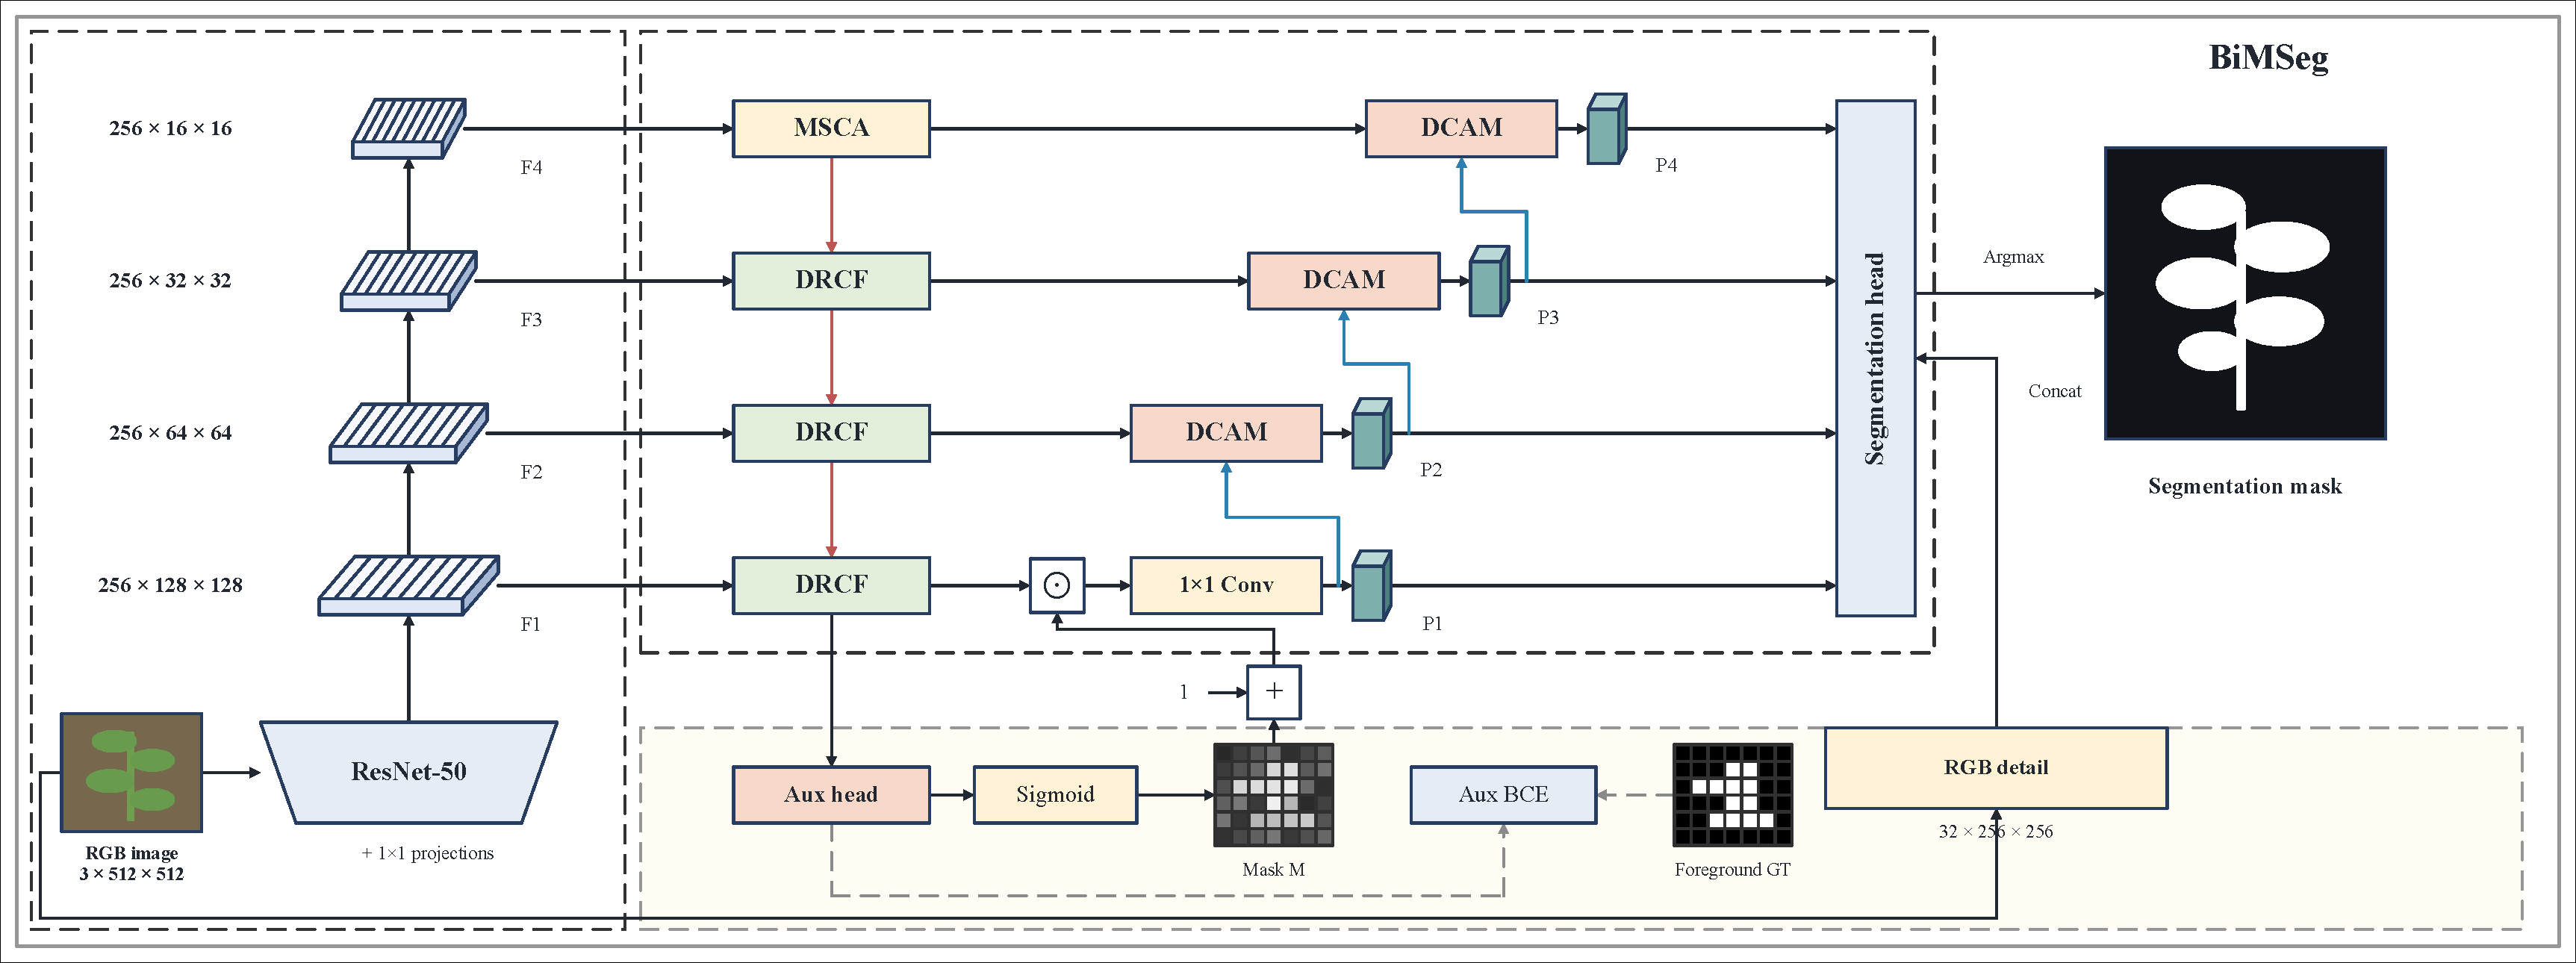
\includegraphics[width=\linewidth]{BiMSeg_Architecture_Polished.pdf}\par
  \begin{spacing}{1}
    \methodbicaption{BiMSeg 整体网络架构}
      {Overall architecture of BiMSeg}{fig:architecture}
  \end{spacing}
  \par
\endgroup
\addvspace{6pt}

针对禾本科植物图像中目标尺度变化、叶片相互遮挡及细长结构
难以完整分割的问题，本文提出双向多尺度分割网络
（Bidirectional Multi-scale Segmentation Network，BiMSeg）。
网络由 ResNet50 编码器、多尺度稀疏交叉注意力模块
（Multi-scale Sparse Cross-Attention，MSCA）、
动态关系与上下文融合模块
（Dynamic Relation and Context Fusion，DRCF）、
差异引导的跨尺度自适应调制模块
（Discrepancy-guided Cross-scale Adaptive Modulation，DCAM）
及分割预测头组成。
通过自顶向下的语义传递与自底向上的细节反馈，
实现深层语义、浅层结构及图像细节的协同整合。

如图~\ref{fig:architecture} 所示，
给定输入图像 \(I\in\mathbb{R}^{3\times H\times W}\)，
采用 ResNet50 编码器\papercite{he2016resnet}
提取四个层级的特征，
并通过 \(1\times1\) 卷积将通道数统一为 \(C=256\)，
得到特征集合 \(\{F_1,F_2,F_3,F_4\}\)。
其空间分辨率依次为输入的
\(1/4\)、\(1/8\)、\(1/16\) 和 \(1/32\)。
最深层特征 \(F_4\) 经 MSCA
聚合多尺度局部信息与空间上下文，
得到增强特征 \(F_4'\)，
并令 \(G_4=F_4'\)。
随后，三级 DRCF 分别融合
\(G_4\) 与 \(F_3\)、\(G_3\) 与 \(F_2\)、
\(G_2\) 与 \(F_1\)，
依次生成 \(G_3\)、\(G_2\) 和 \(G_1\)，
完成自顶向下的语义传递。
为简化表示，后续特征尺寸描述中省略批量维度。

基于最浅层融合特征 \(G_1\)，
辅助预测头生成前景概率图 \(M\)，
通过残差加权增强前景响应，
并经通道映射得到 \(P_1\)。
自底向上路径以 \(P_1\) 为起点，
利用三级 DCAM 分别与 \(G_2\)、\(G_3\) 和 \(G_4\)
交互，依次生成 \(P_2\)、\(P_3\) 和 \(P_4\)，
将浅层细节逐级反馈至深层表征。
最后，对齐并融合四个层级的输出，
结合 RGB 细节分支生成与输入图像等分辨率的类别响应，
得到最终分割结果。

\subsubsection{多尺度稀疏交叉注意力模块（MSCA）}
\begingroup
  \centering
  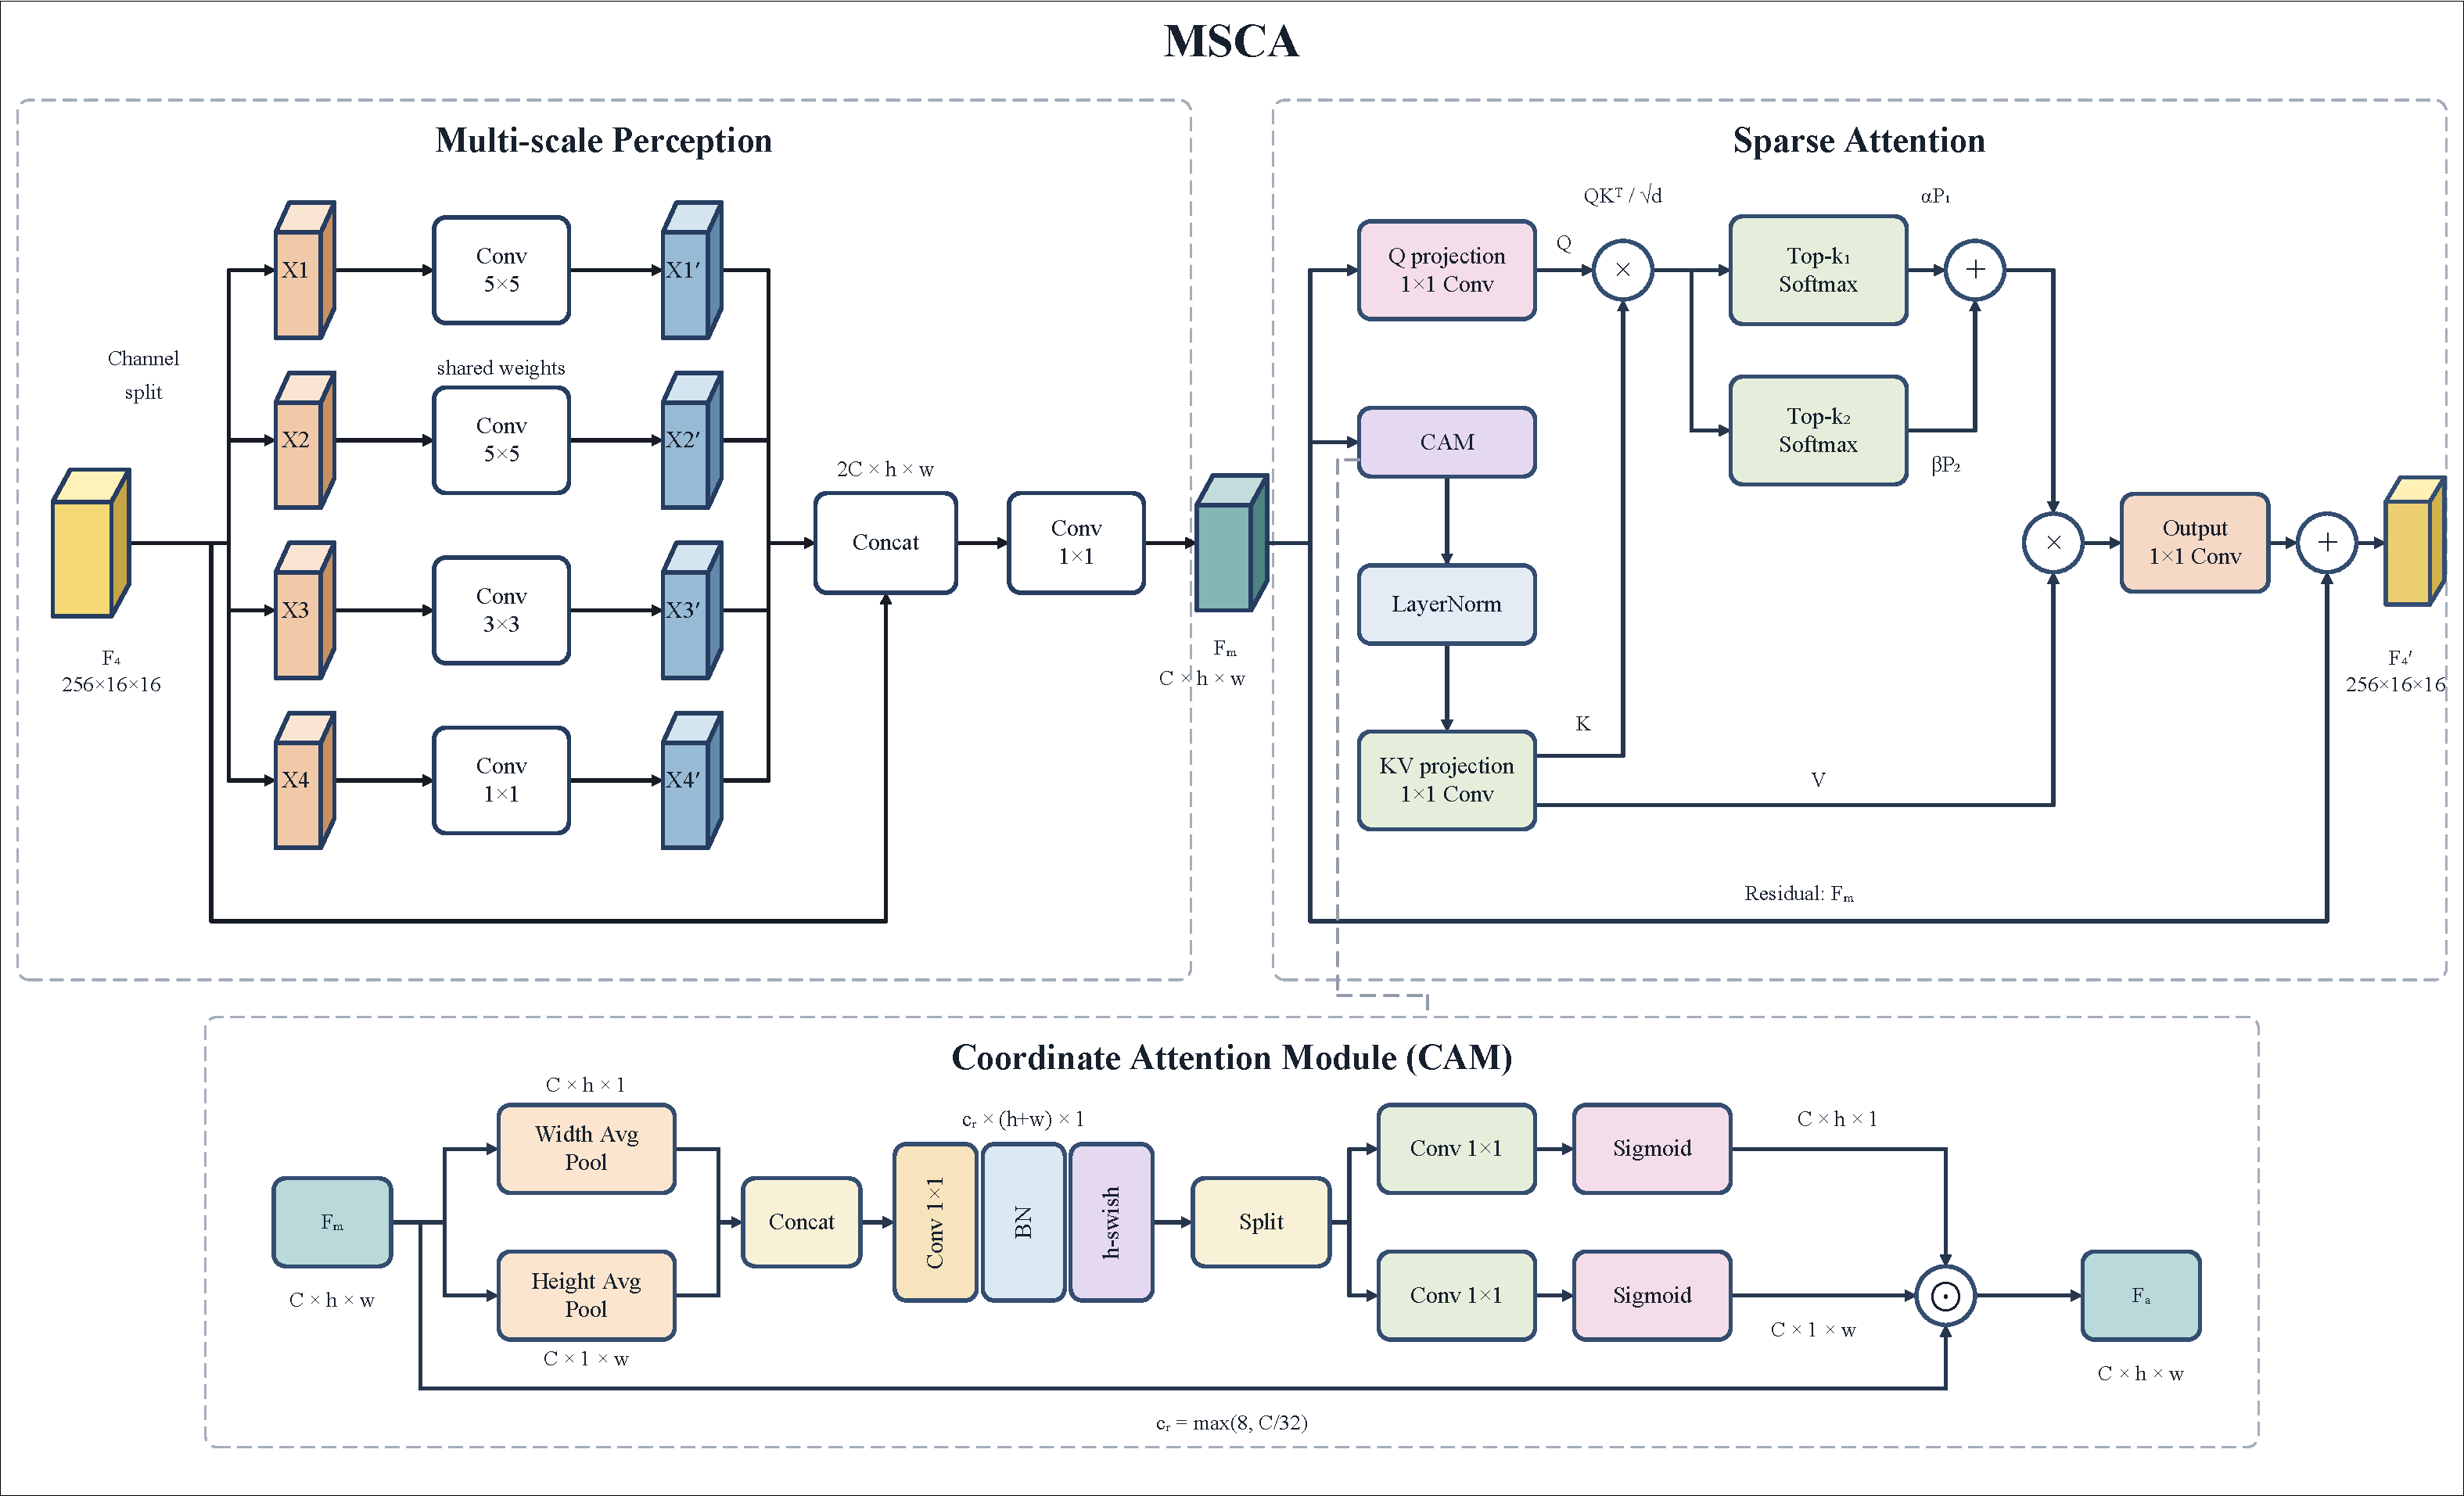
\includegraphics[width=\linewidth]{MSCA_CAM_Editable.pdf}\par
  \begin{spacing}{1}
    \methodbicaption{多尺度稀疏交叉注意力模块（MSCA）}
      {Multi-scale sparse cross-attention module (MSCA)}{fig:msca}
  \end{spacing}
  \par
\endgroup
\addvspace{6pt}

植物叶片的尺度差异与相互遮挡要求网络
同时表征局部结构和远距离空间关联。
为此，本文构建多尺度稀疏交叉注意力模块。
如图~\ref{fig:msca} 所示，
MSCA 首先提取并融合不同邻域范围的特征，
随后以融合表征生成查询，
以坐标注意力增强后的表征生成键和值，
通过双分支稀疏聚合完成空间信息交互。
该设计将多尺度感知与非对称特征交互结合，
使局部融合表征与注意力增强表征
在匹配和聚合过程中承担不同作用。

\noindent\textbf{多尺度感知}\par

在 MPCNet 的多尺度感知结构
\papercite{zhang2026mpcnet} 基础上，
将分支卷积核配置调整为 \(5\)、\(5\)、\(3\)、\(1\)，
构建用于深层特征处理的多尺度映射。
给定 \(F_4\in\mathbb{R}^{C\times h\times w}\)，
沿通道维度将其均分为四组
\(X_i\in\mathbb{R}^{(C/4)\times h\times w}\)，
分别进行卷积变换：

\begin{equation}
X_i'=\phi_{s_i}(X_i),\quad
(s_1,s_2,s_3,s_4)=(5,5,3,1)
\label{eq:msca-branches}
\end{equation}

其中，\(\phi_{s_i}\) 表示对应的卷积映射。
两个 \(5\times5\) 分支共享卷积参数，
对不同通道子集执行一致的空间变换；
\(3\times3\) 分支提取较小邻域内的结构信息，
\(1\times1\) 分支执行逐位置的通道变换。
各分支保持空间分辨率不变，
输出与原始特征沿通道维度拼接，
再通过 \(1\times1\) 卷积融合：

\begin{equation}
F_m=\phi_f\left(
\operatorname{Concat}[F_4,X_1',X_2',X_3',X_4']
\right)
\label{eq:msca-fusion}
\end{equation}

拼接特征具有 \(2C\) 个通道，
经融合映射恢复至 \(C\) 个通道，
得到 \(F_m\in\mathbb{R}^{C\times h\times w}\)。
该结构在保留原始深层表征的同时，
整合不同邻域范围内的特征响应，
为后续空间交互提供多尺度查询依据。

\noindent\textbf{坐标注意力引导的交叉注意力}\par

为在特征重标定过程中保留空间位置信息，
采用坐标注意力机制\papercite{hou2021coordinate}
构成坐标注意力模块
（Coordinate Attention Module，CAM）。
该模块分别沿宽度和高度方向进行平均池化，
经共享变换与方向分解生成两组注意力权重，
并以广播方式作用于融合特征，
得到增强表征 \(F_a\)。

以 \(F_m\) 生成查询，
以 \(F_a\) 经层归一化后的表征生成键和值：

\begin{equation}
Q=\phi_q(F_m),\quad
[K,V]=\operatorname{Split}\left(
\phi_{kv}(\operatorname{LN}(F_a))
\right)
\label{eq:msca-qkv}
\end{equation}

查询投影与键值投影均采用 \(1\times1\) 卷积，
输出通道数分别为 \(C\) 和 \(2C\)；
后者沿通道维度拆分为键和值。
层归一化在每个空间位置沿通道维度执行。
查询保留多尺度融合特征，
键和值则来自坐标注意力增强后的表征，
从而在共同的空间网格上建立
两种特征表示之间的非对称关联。

随后，对查询、键和值进行空间展平与多头重排。
设空间位置数为 \(N=hw\)，
注意力头数为 \(n_h\)，
单头通道维度为 \(d=C/n_h\)。
为简化记号，
单头特征仍记为
\(Q,K,V\in\mathbb{R}^{N\times d}\)，
其相关性矩阵为：

\begin{equation}
S=\frac{QK^{\mathsf T}}{\sqrt{d}}
\label{eq:msca-scores}
\end{equation}

矩阵 \(S\in\mathbb{R}^{N\times N}\)
描述查询位置与键位置之间的相关性，
缩放因子 \(\sqrt{d}\) 用于调节点积幅值。

\noindent\textbf{双分支稀疏聚合}\par

基于 MSCN 的双分支稀疏聚合机制
\papercite{ma2025mscn}，
对相关性矩阵采用两种保留比例进行逐行筛选，
构建不同连接密度的注意力分支：

\begin{equation}
\mathsf{P}_r=\operatorname{Softmax}\left(
\mathcal{T}_{k_r}(S)
\right),\quad r\in\{1,2\}
\label{eq:msca-sparse}
\end{equation}

权重矩阵
\(\mathsf{P}_r\in\mathbb{R}^{N\times N}\)
对应第 \(r\) 路稀疏注意力。
保留数量分别为
\(k_1=\max(1,\lfloor N/2\rfloor)\)
和 \(k_2=\max(1,\lfloor N/6\rfloor)\)。
算子 \(\mathcal{T}_{k_r}\)
保留每行最大的 \(k_r\) 个元素，
将其余元素置为负无穷；
Softmax 沿键位置维度执行，
使未保留位置的注意力权重为零。
两条分支分别提供较广泛与较集中的空间关联，
经可学习系数融合后作用于值特征：

\begin{equation}
Z=(\alpha\mathsf{P}_1+\beta\mathsf{P}_2)V
\label{eq:msca-aggregation}
\end{equation}

系数 \(\alpha\) 和 \(\beta\) 均初始化为 0.5，
用于学习两种聚合结果的贡献。
最后，拼接各注意力头的输出并恢复空间排列，
经 \(1\times1\) 卷积投影后
与融合特征残差相加：

\begin{equation}
F_4'=F_m+\phi_o\left(
\operatorname{Merge}(Z)
\right)
\label{eq:msca-output}
\end{equation}

\(\operatorname{Merge}\) 表示多头拼接与空间恢复。
输出 \(F_4'\in\mathbb{R}^{C\times h\times w}\)
保持输入尺寸，
通过残差连接整合多尺度融合表征
与稀疏聚合的空间上下文，
并作为自顶向下路径的起始特征 \(G_4\)。

\subsubsection{动态关系与上下文融合模块（DRCF）}
\begingroup
  \centering
  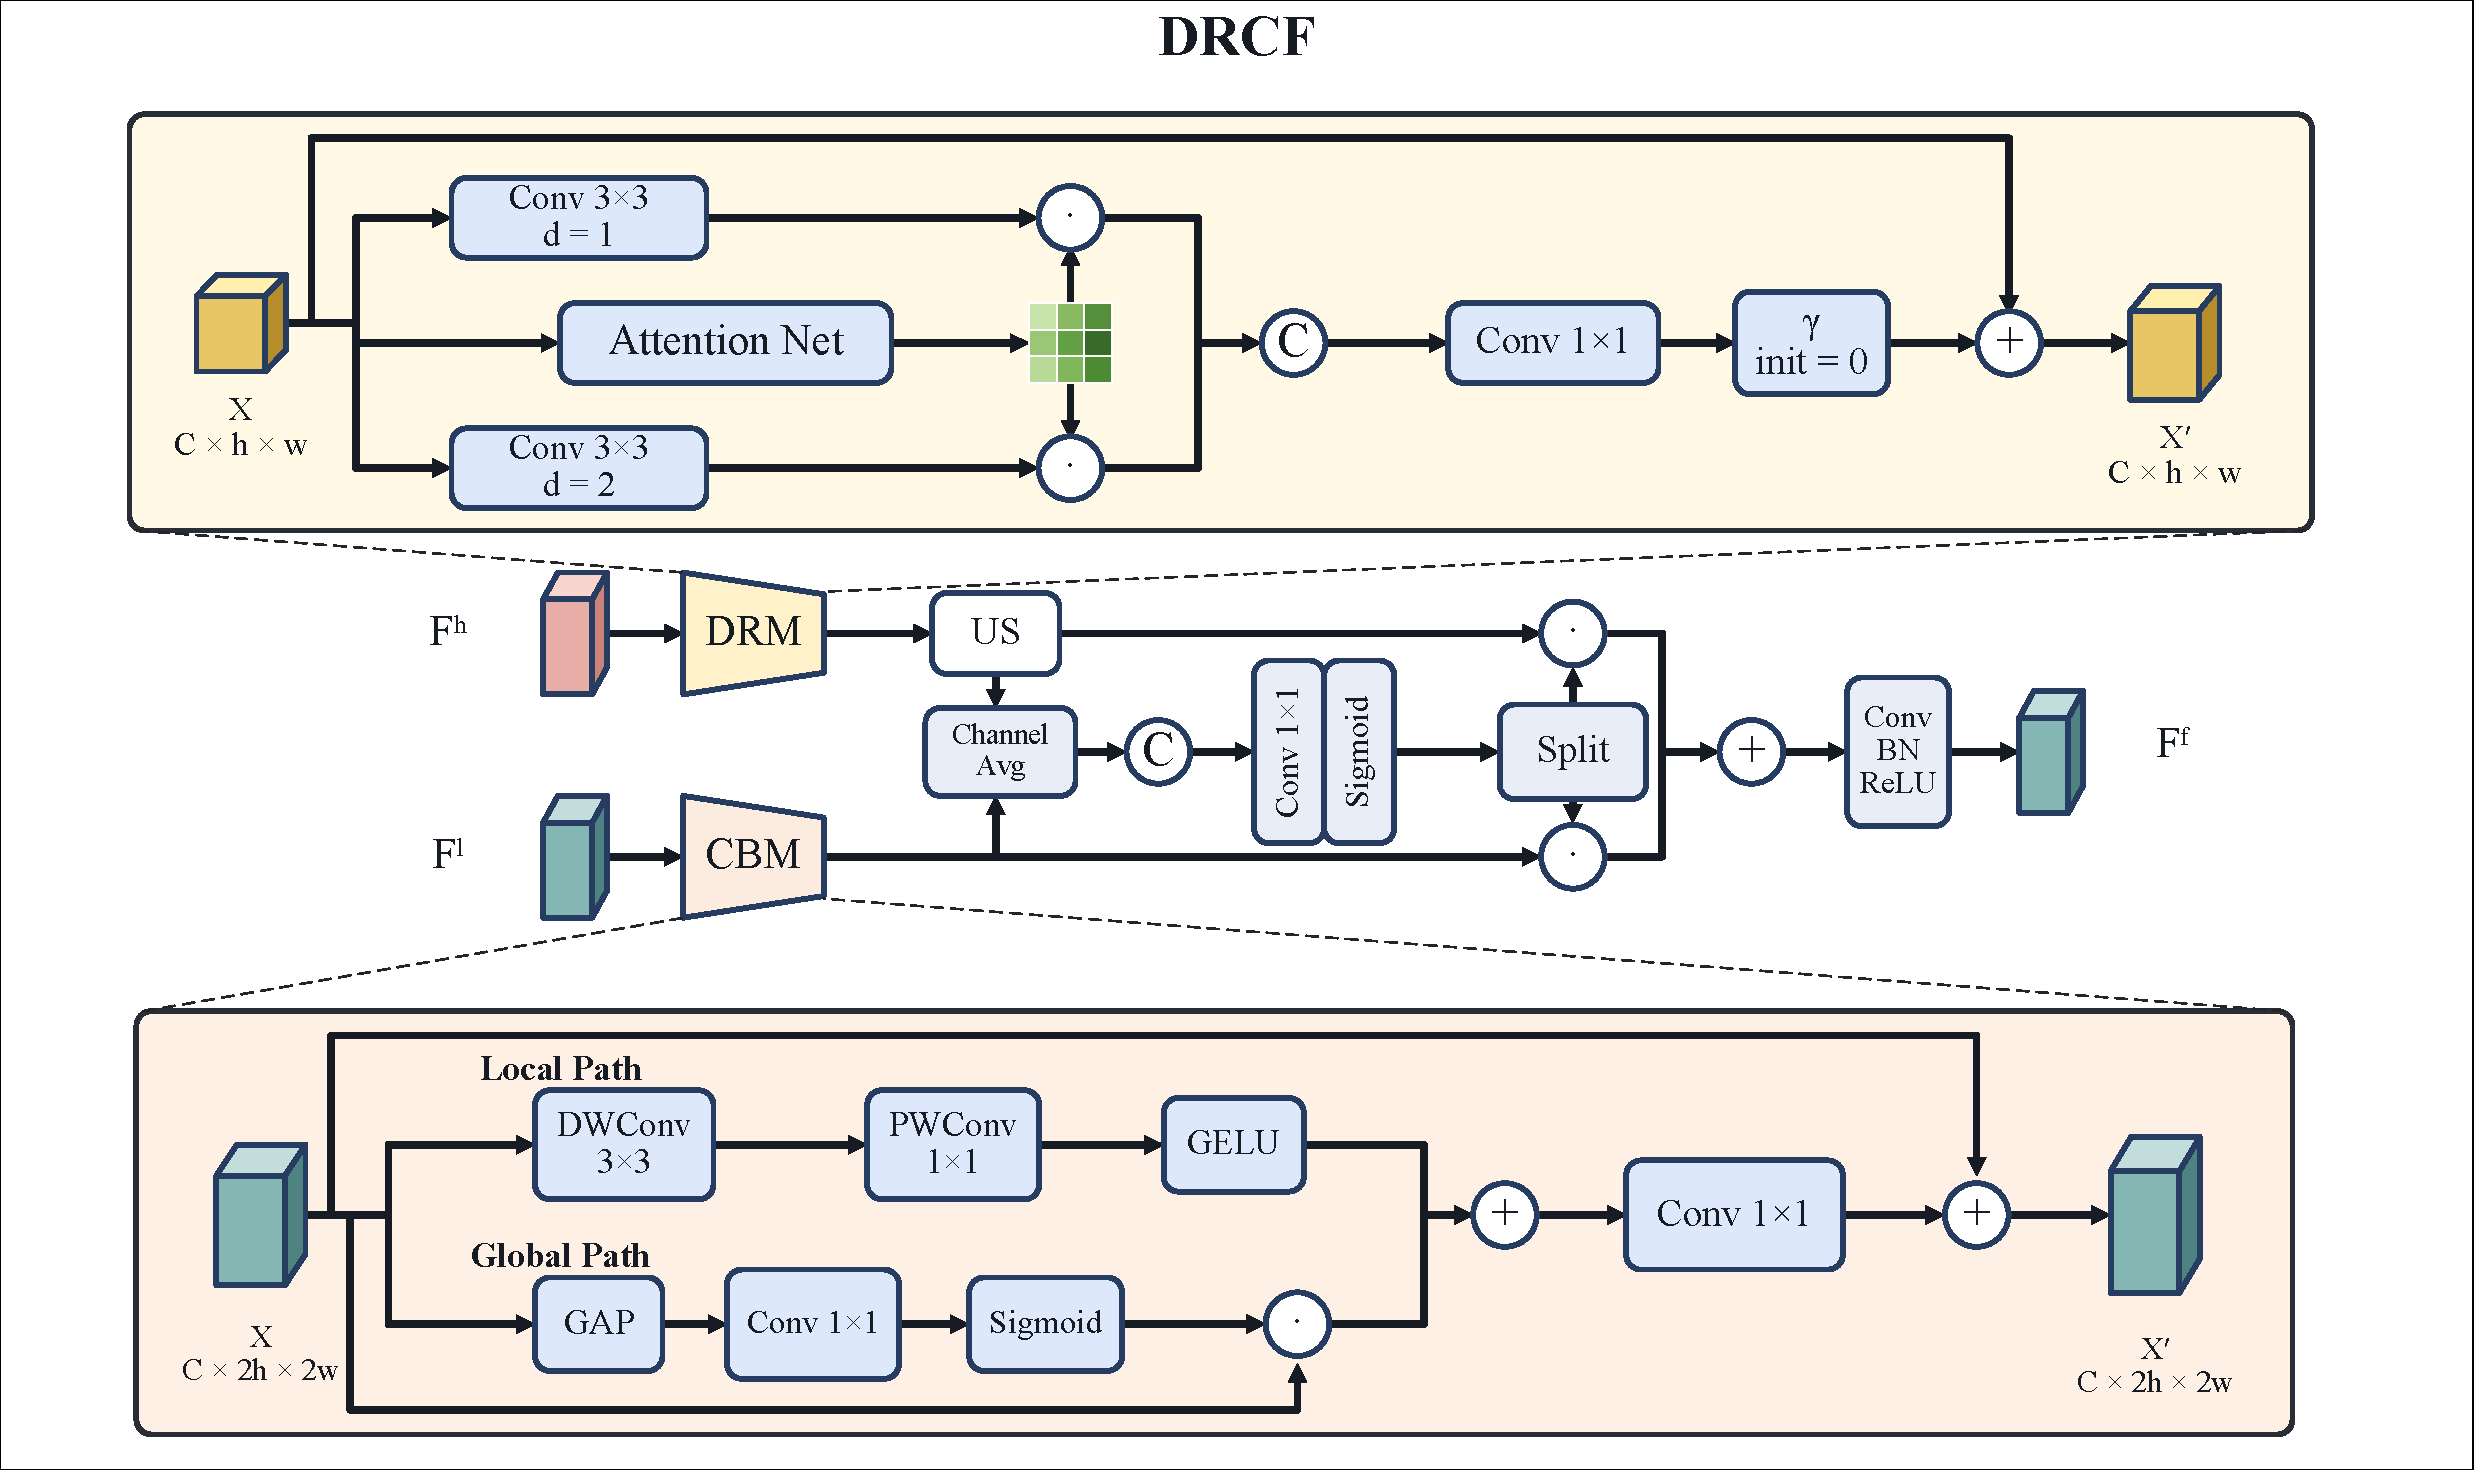
\includegraphics[width=\linewidth]{DRCF_MODA_Style.pdf}\par
  \begin{spacing}{1}
    \methodbicaption{动态关系与上下文融合模块（DRCF）}
      {Dynamic relation and context fusion module (DRCF)}{fig:drcf}
    \par\smallskip
    {\zihao{5}\normalfont
     注：上、下展开部分分别为 DRM 和 CBM；绿色方格表示
     DRM 的分支权重，对应两个经 Softmax 归一化的样本级标量。\par 
     Note: The upper and lower insets show DRM and CBM, respectively.
     The green squares represent the DRM branch weights, which are two
     sample-specific scalars normalized by softmax.\par}
  \end{spacing}
  \par
\endgroup
\addvspace{6pt}

不同层级特征在空间分辨率与语义表征上存在差异：
深层特征具有较强的语义信息，
浅层特征保留更多局部纹理与边界细节。
为实现两类信息的自适应整合，
本文构建动态关系与上下文融合模块。
采用 HyperSeg-DG 中的动态关系模块
（Dynamic Relation Module，DRM）
与上下文桥接模块
（Context Bridge Module，CBM）
\papercite{islam2026hypersegdg}
分别处理深、浅层输入，
并根据两路增强特征的空间响应
生成跨尺度融合权重。

如图~\ref{fig:drcf} 所示，
DRCF 将深层动态关系建模、
浅层上下文增强及空间自适应融合结合，
在不同分辨率之间传递语义与结构信息。
三级 DRCF 依次融合
\(G_4\) 与 \(F_3\)、\(G_3\) 与 \(F_2\)、
\(G_2\) 与 \(F_1\)，
生成 \(G_3\)、\(G_2\) 和 \(G_1\)。

\noindent\textbf{深层特征的动态关系建模}\par

给定深层输入
\(F_h\in\mathbb{R}^{C\times h\times w}\)，
采用两路膨胀率分别为 1 和 2 的
\(3\times3\) 卷积，
提取不同感受野下的特征：

\begin{equation}
D_r=\phi_{3\times3}^{(r)}(F_h),\quad r\in\{1,2\}
\label{eq:drcf-dilated}
\end{equation}

为根据输入内容调整两路响应，
利用全局平均池化提取通道描述，
经两层 \(1\times1\) 卷积与 ReLU 激活
生成分支得分，
再通过 Softmax 得到权重：

\begin{equation}
[a_1,a_2]=\operatorname{Softmax}\left(
\psi_2\left(
\operatorname{ReLU}\left(
\psi_1(\operatorname{GAP}(F_h))
\right)\right)\right)
\label{eq:drcf-branch-weights}
\end{equation}

权重 \(a_1\) 和 \(a_2\)
为随输入变化的样本级标量，
满足 \(a_1+a_2=1\)，
在通道与空间维度广播后
分别作用于两路特征。
加权结果经拼接与 \(1\times1\) 卷积融合，
再通过可学习残差系数与原始输入结合：

\begin{equation}
H=F_h+\gamma\,\phi_d\left(
\operatorname{Concat}[a_1D_1,a_2D_2]
\right)
\label{eq:drcf-drm-output}
\end{equation}

系数 \(\gamma\) 初始化为零，
使 DRM 在初始化时保持恒等映射，
并在训练过程中学习
多感受野特征对输出的贡献。

\noindent\textbf{浅层特征的上下文增强}\par

对于浅层输入
\(F_l\in\mathbb{R}^{C\times2h\times2w}\)，
CBM 通过并行的局部路径与全局路径
提取互补信息。
局部路径采用深度卷积与逐点卷积
建模邻域结构，
全局路径通过全局平均池化与 Sigmoid
生成通道门控：

\begin{equation}
L_{\mathrm{loc}}=\operatorname{GELU}\left(
\phi_{\mathrm{pw}}(\phi_{\mathrm{dw}}(F_l))
\right),\quad
g=\sigma\left(
\phi_g(\operatorname{GAP}(F_l))
\right)
\label{eq:drcf-local-global}
\end{equation}

其中，
\(\phi_{\mathrm{dw}}\) 为 \(3\times3\) 深度卷积，
\(\phi_{\mathrm{pw}}\) 为 \(1\times1\) 逐点卷积，
\(g\in\mathbb{R}^{C\times1\times1}\)
为通道门控权重。
全局路径将门控作用于原始浅层特征，
与局部路径输出相加，
经投影及残差连接得到增强特征：

\begin{equation}
L=F_l+\phi_c\left(
L_{\mathrm{loc}}+g\odot F_l
\right)
\label{eq:drcf-cbm-output}
\end{equation}

该结构在保留浅层输入的基础上，
结合局部空间变换与全局通道调节，
为跨层融合提供上下文增强的细节表征。
符号 \(\odot\) 表示逐元素乘法，
不同尺寸的权重按相应维度广播。

\noindent\textbf{空间自适应融合}\par

将深层输出双线性上采样至浅层分辨率，
得到 \(H'=\operatorname{Up}(H)\)。
随后，分别沿通道维度计算两路特征的均值，
生成单通道空间描述图：

\begin{equation}
S_h=\operatorname{Mean}_c(H'),\quad
S_l=\operatorname{Mean}_c(L)
\label{eq:drcf-spatial-descriptors}
\end{equation}

将两张描述图拼接，
通过 \(1\times1\) 卷积与 Sigmoid
预测空间融合权重：

\begin{equation}
[W_h,W_l]=\operatorname{Split}\left(
\sigma\left(
\phi_w\left(
\operatorname{Concat}[S_h,S_l]
\right)\right)\right)
\label{eq:drcf-spatial-weights}
\end{equation}

权重
\(W_h,W_l\in\mathbb{R}^{1\times2h\times2w}\)
由 Sigmoid 独立生成，
在通道维度广播，
分别调节各空间位置的深层与浅层响应。
两路加权特征相加后，
经 \(1\times1\) 卷积、
批归一化与 ReLU 激活得到模块输出：

\begin{equation}
F_{\mathrm{DRCF}}=\operatorname{ReLU}\left(
\operatorname{BN}\left(
\phi_f(W_h\odot H'+W_l\odot L)
\right)\right)
\label{eq:drcf-output}
\end{equation}

输出
\(F_{\mathrm{DRCF}}\in\mathbb{R}^{C\times2h\times2w}\)
与浅层输入保持相同尺寸。
通过对深浅层特征分别增强并自适应加权，
DRCF 逐级将深层语义传递至高分辨率表征。

\subsubsection{差异引导的跨尺度自适应调制模块（DCAM）}
\begingroup
  \centering
  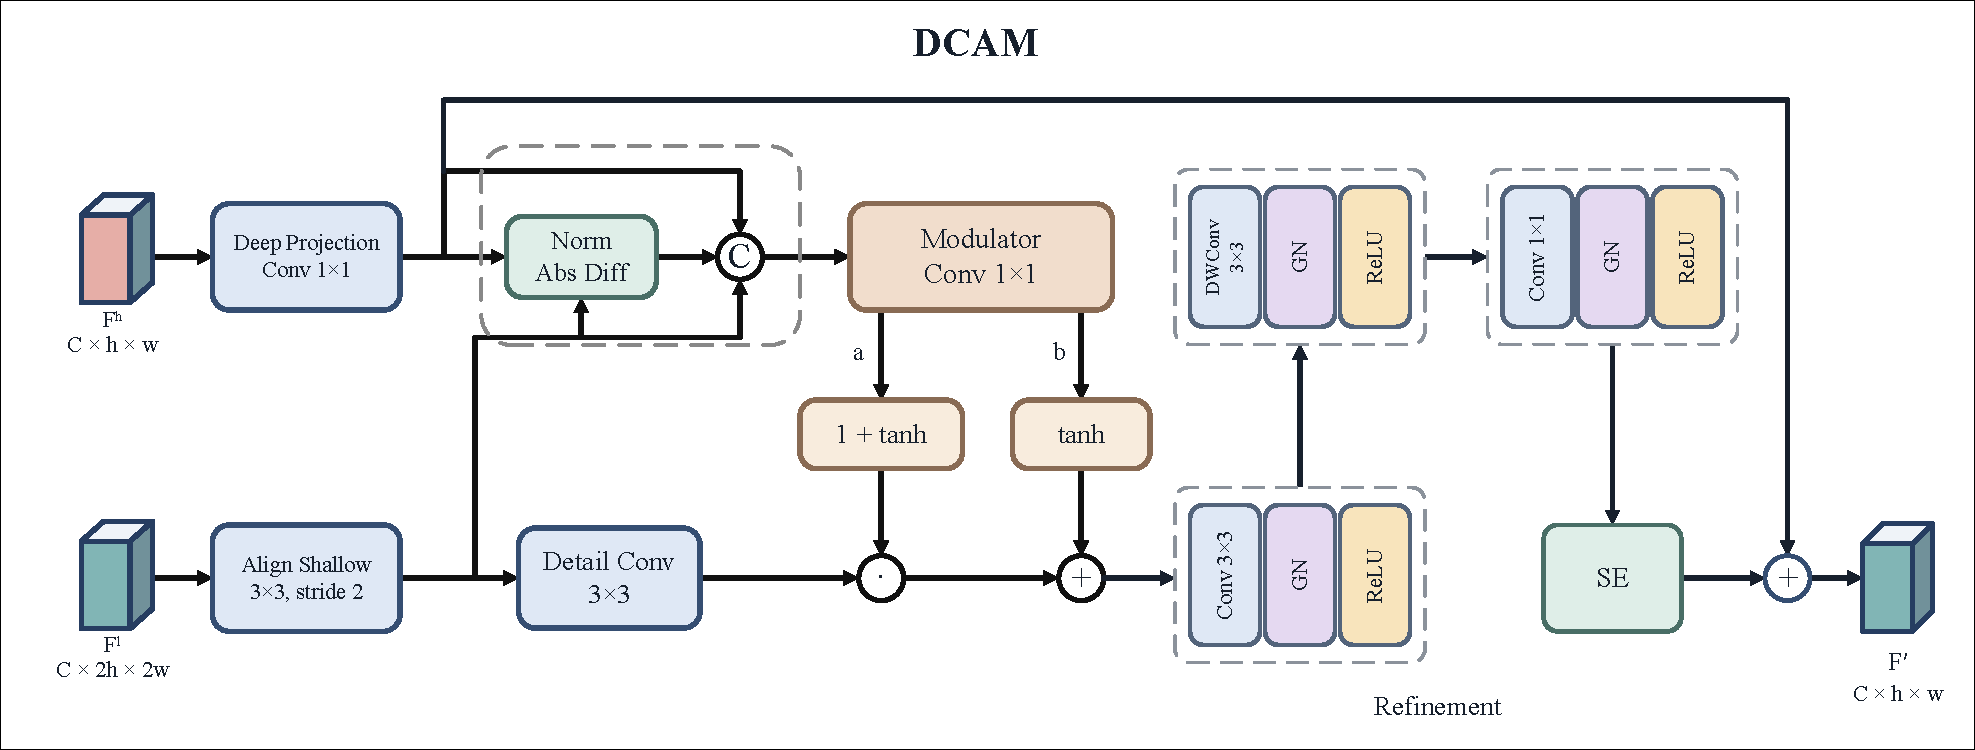
\includegraphics[width=\linewidth]{DCAM_Aligned_Editable.pdf}\par
  \begin{spacing}{1}
    \methodbicaption{差异引导的跨尺度自适应调制模块（DCAM）}
      {Difference-guided cross-scale adaptive modulation module (DCAM)}{fig:dcam}
  \end{spacing}
  \par
\endgroup
\addvspace{6pt}

跨尺度特征融合需要协调
深层语义与浅层细节之间的表征差异。
直接叠加两类特征
缺乏依据局部差异调节信息注入强度的机制。
为此，本文构建差异引导的跨尺度自适应调制模块。
如图~\ref{fig:dcam} 所示，
模块利用对齐特征及其归一化差异
生成通道与空间相关的调制参数，
对浅层细节进行乘性缩放与加性偏移，
再通过残差细化完成跨尺度信息整合。

\noindent\textbf{跨尺度特征对齐}\par

给定深层特征
\(F_h\in\mathbb{R}^{C\times h\times w}\)
和浅层特征
\(F_l\in\mathbb{R}^{C\times2h\times2w}\)，
分别通过深层投影与浅层对齐得到：

\begin{equation}
T=\phi_p(F_h),\quad S=\phi_a(F_l)
\label{eq:dcam-alignment}
\end{equation}

深层投影 \(\phi_p\)
采用 \(1\times1\) 卷积进行通道映射；
浅层对齐 \(\phi_a\)
采用步长为 2 的 \(3\times3\) 卷积，
结合组归一化与 ReLU 激活完成下采样。
两路输出均为 \(C\times h\times w\)，
为逐位置差异计算与特征调制
建立统一的空间和通道维度。

\noindent\textbf{差异引导的调制参数生成}\par

为减弱特征幅值差异对比较结果的影响，
在每个空间位置沿通道维度进行 \(L_2\) 归一化，
再计算两路特征的逐元素绝对差异：

\begin{equation}
D=\left|\mathcal{N}(S)-\mathcal{N}(T)\right|
\label{eq:dcam-discrepancy}
\end{equation}

归一化算子定义为
\(\mathcal{N}(U)_{:,i,j}
=U_{:,i,j}/\max(\lVert U_{:,i,j}\rVert_2,\epsilon)\)，
其中 \(U_{:,i,j}\)
表示位置 \((i,j)\) 处的通道向量，
\(\epsilon\) 为数值稳定常数。
差异特征
\(D\in\mathbb{R}^{C\times h\times w}\)
描述两路表征在归一化通道响应上的差异。
将其与对齐特征拼接，
通过 \(1\times1\) 卷积生成调制参数：

\begin{equation}
[a,b]=\operatorname{Split}\left(
\phi_m\left(
\operatorname{Concat}[S,T,D]
\right)\right)
\label{eq:dcam-modulation-parameters}
\end{equation}

拼接特征具有 \(3C\) 个通道，
经调制映射 \(\phi_m\) 转换为 \(2C\) 个通道，
再拆分为
\(a,b\in\mathbb{R}^{C\times h\times w}\)。
两组参数由深浅层特征及其差异共同生成，
用于调节各通道、各空间位置的细节响应，
使浅层信息的注入强度随输入内容变化。

\noindent\textbf{细节调制与残差细化}\par

对浅层对齐特征进行 \(3\times3\) 卷积、
组归一化与 ReLU 激活，
得到细节特征 \(E=\phi_e(S)\)。
利用调制参数分别执行乘性缩放与加性偏移：

\begin{equation}
E'=E\odot\left(1+\tanh(a)\right)+\tanh(b)
\label{eq:dcam-modulation}
\end{equation}

乘性系数 \(1+\tanh(a)\)
的取值范围为 \((0,2)\)，
用于调节细节响应强度；
偏移项 \(\tanh(b)\)
的取值范围为 \((-1,1)\)，
提供加性调整。
调制卷积 \(\phi_m\) 的权重与偏置均初始化为零，
使初始调制满足 \(E'=E\)，
训练过程中再学习偏离恒等调制的幅度。

调制结果依次经过 \(3\times3\) 卷积、
\(3\times3\) 深度卷积和 \(1\times1\) 逐点卷积，
各卷积后均接组归一化与 ReLU 激活。
随后，采用挤压与激励单元
（Squeeze-and-Excitation，SE）
\papercite{hu2018senet}
进行通道重标定，得到细化特征：

\begin{equation}
R=\operatorname{SE}\left(
\rho_{\mathrm{pw}}\left(
\rho_{\mathrm{dw}}\left(
\rho_{3\times3}(E')
\right)\right)\right)
\label{eq:dcam-refinement}
\end{equation}

其中，
\(\rho_{3\times3}\)、\(\rho_{\mathrm{dw}}\)
和 \(\rho_{\mathrm{pw}}\)
分别表示上述三类卷积及其归一化、激活操作。
最终将细化结果与深层投影特征残差相加：

\begin{equation}
F'=T+R
\label{eq:dcam-output}
\end{equation}

模块输出与深层输入保持相同尺寸，
以深层投影特征为残差基础，
整合经过差异引导调制与细化的浅层信息。
在自底向上路径中，
三级 DCAM 分别以
\(G_2\)、\(G_3\) 和 \(G_4\) 为深层输入，
以 \(P_1\)、\(P_2\) 和 \(P_3\) 为浅层输入，
依次生成 \(P_2\)、\(P_3\) 和 \(P_4\)，
完成浅层细节向深层表征的逐级反馈。

\subsubsection{分割输出与损失函数}

\noindent\textbf{前景辅助监督与残差增强}\par

在自顶向下路径的最浅层融合特征 \(G_1\)
上设置辅助预测头，
生成单通道前景响应 \(A\)，
经 Sigmoid 得到前景概率图 \(M\)。
利用前景概率对融合特征进行残差加权，
再通过通道映射形成
自底向上路径的起始特征：

\begin{equation}
A=\phi_{\mathrm{aux}}(G_1),\quad
M=\sigma(A),\quad
P_1=\phi_s\left(G_1\odot(1+M)\right)
\label{eq:prediction-foreground}
\end{equation}

辅助预测头由 \(3\times3\) 卷积、
组归一化、ReLU 和 \(1\times1\) 输出卷积组成。
概率图 \(M\) 在通道维度广播，
使残差加权在保留原始特征分量的基础上
增强前景响应。
随后，三级 DCAM 逐级融合浅层细节与深层语义，
生成 \(P_2\)、\(P_3\) 和 \(P_4\)。

\noindent\textbf{多尺度解码与细节融合}\par

将 \(P_1\) 至 \(P_4\)
对齐至输入图像的四分之一分辨率，
沿通道维度拼接后，
通过卷积解码器得到融合特征 \(U\)。
同时，将输入图像缩放至二分之一分辨率，
通过 RGB 细节分支提取局部特征
\(E_{\mathrm{rgb}}\)。
解码特征上采样后与细节特征拼接，
经分割预测头生成类别响应，
并恢复至输入尺寸：

\begin{equation}
O=\mathcal{U}_1\left(
\phi_{\mathrm{seg}}\left(
\operatorname{Concat}[
\mathcal{U}_{1/2}(U),E_{\mathrm{rgb}}
]\right)\right)
\label{eq:prediction-output}
\end{equation}

其中，
\(\mathcal{U}_{1/2}\) 和 \(\mathcal{U}_1\)
分别表示对齐至输入图像二分之一分辨率
和原始分辨率的双线性插值。
解码器通过两个 \(3\times3\) 卷积块，
将拼接特征的通道数依次压缩至 256 和 64；
RGB 分支通过两个 \(3\times3\) 卷积块
生成 32 通道细节特征。
分割预测头由 \(3\times3\) 卷积块
和 \(1\times1\) 分类卷积组成。
本节中的卷积块均由卷积、
组归一化与 ReLU 激活组成。
最终输出为
\(O\in\mathbb{R}^{K\times H\times W}\)，
其中 \(K\) 为包含背景的类别总数。
推理时，选取各像素最大类别响应
对应的类别作为分割结果。

\noindent\textbf{联合训练目标}\par

主分割分支采用像素级交叉熵损失
与前景 Dice 损失联合监督。
交叉熵约束像素类别预测，
Dice 损失约束预测区域与真实区域的重叠，
对每幅图像的各前景类别分别计算后，
在样本与类别维度取平均：

\begin{equation}
\mathcal{L}_{\mathrm{Dice}}
=1-\frac{1}{B(K-1)}
\sum_{b=1}^{B}\sum_{c=1}^{K-1}
\frac{2\sum_i p_{bic}y_{bic}+\epsilon_d}
{\sum_i p_{bic}+\sum_i y_{bic}+\epsilon_d}
\label{eq:loss-dice}
\end{equation}

其中，\(B\) 为批量大小，
\(i\) 遍历图像中的像素，
\(c\) 表示类别；
\(p_{bic}\) 为对输出 \(O\)
沿类别维度执行 Softmax 后得到的预测概率，
\(y_{bic}\) 为对应的独热标签。
背景类别编号为 0，不参与 Dice 平均，
平滑项设置为 \(\epsilon_d=1\)。

辅助分支将所有非背景类别合并为前景，
采用二元交叉熵监督
上采样至标签分辨率的辅助响应 \(A\)。
训练时直接根据辅助响应计算带 logits 的二元交叉熵，
以提高数值稳定性。
最终训练目标为：

\begin{equation}
\mathcal{L}
=\mathcal{L}_{\mathrm{CE}}
+\lambda_d\mathcal{L}_{\mathrm{Dice}}
+\lambda_a\mathcal{L}_{\mathrm{aux}}
\label{eq:loss-total}
\end{equation}

设置 \(\lambda_d=1\)、\(\lambda_a=0.2\)。
主分割监督共同约束像素类别与前景区域重叠，
辅助监督为前景增强分支提供直接的区域约束，
三者联合优化网络参数。
\par
\endgroup
% !TeX root = main.tex
% 本文件只包含实验正文，请通过 main.tex 编译。

% 第二章：公共数据集实验
% 双语表题沿用 main.tex 中已声明的五号题注字体 methodfive。
\newcommand{\experimentbicaption}[3]{%
  \begingroup
  \captionsetup{position=top,font=methodfive,labelfont=bf,textfont=bf,
    justification=centering,singlelinecheck=false,skip=6pt}%
  \caption[#1]{#1\protect\\Table~\thetable\quad #2}%
  \label{#3}%
  \endgroup
}

\begingroup
\ctexset{
  subsection = {beforeskip = 12pt, afterskip = 8pt},
  subsubsection = {beforeskip = 12pt, afterskip = 8pt}
}

\subsection{公开数据集上的实验与结果}
\label{sec:experiments}

为评价 BiMSeg 在不同作物与分割任务中的表现，本文选用三个公开作物图像分割数据集开展实验：在 VegAnn（小麦、水稻、玉米、向日葵等多种作物）\papercite{madec2023vegann} 上评价植被前景提取性能，在 GWFSS（小麦）\papercite{wang2025gwfss} 上评价叶片、茎秆与麦穗的器官分割性能，在 RiceSEG（水稻）\papercite{zhou2025riceseg} 上评价稻田场景的多类别分割性能。通过对比实验比较 BiMSeg 与现有方法的分割精度和推理效率，并通过消融实验分析各模块及其组合对分割性能的影响。上述实验为后续黑麦草冠层分割与模型辅助标注提供方法依据。

\subsubsection{实验设置}
\label{sec:exp-settings}
\medskip\noindent\textbf{数据集与数据划分}\par
\label{sec:exp-datasets}
本文选用 VegAnn、GWFSS 和 RiceSEG 三个公开作物图像分割数据集，分别评价 BiMSeg 在多作物植被前景提取、小麦器官分割和水稻田间场景多类别分割任务中的表现。\par
植被标注数据集（Vegetation Annotation，VegAnn）包含 3775 张 RGB 图像，覆盖小麦、水稻、玉米和向日葵等 26 种作物类型，涉及不同生育阶段、成像平台和光照条件，采用植被前景与背景两类标注\papercite{madec2023vegann}。全球小麦器官语义分割数据集（Global Wheat Full Semantic Organ Segmentation，GWFSS）包含 1096 张像素级标注的小麦图像，区分麦穗、茎、叶和背景四类，用于评价模型对交叠器官及细长茎叶的识别能力\papercite{wang2025gwfss}。全球水稻多类别分割数据集（Global Rice Multiclass Segmentation，RiceSEG）包含 3078 张标注图像，采集自中国、日本、印度、菲律宾和坦桑尼亚，标注类别包括背景、绿色植被、衰老植被、稻穗、杂草和浮萍，用于评价模型对稻田中不同器官、植被类型及组织状态的区分能力\papercite{zhou2025riceseg}。三个数据集的原始图像及对应的分割掩膜示例见图~\ref{fig:public-segmentation-datasets}。
\begin{figure}[H]
  \centering
  \includegraphics[width=0.95\linewidth]{figures/public_segmentation_dataset_examples.pdf}
  \methodbicaption{公开作物图像分割数据集示例}
    {Examples from the public crop image segmentation datasets}
    {fig:public-segmentation-datasets}
  \par\smallskip
  {\raggedright\normalfont\zihao{5}
   \noindent 注：a、b、c 三列分别对应 VegAnn、GWFSS 和 RiceSEG。上排为原始图像，下排为对应的分割掩膜。\par
   \noindent Note: Columns a--c show examples from VegAnn, GWFSS, and RiceSEG, respectively. The top row shows the original images, and the bottom row shows the corresponding segmentation masks.\par}
\end{figure}
VegAnn 采用官方元数据中的 TVT-split1 划分；GWFSS 和 RiceSEG 均按约 \(8:1:1\) 的比例划分训练集、验证集和测试集。训练集用于优化模型参数，验证集用于选择模型检查点，测试集用于最终性能评价。同一数据集上的各对比方法均采用相同的划分。各数据集涉及的作物、类别数及各子集的图像数量见表~\ref{tab:exp-datasets}，其中类别数均包含背景。
\begin{table}[H]
  \centering
  \experimentbicaption{语义分割实验数据集统计与划分}
    {Dataset statistics and splits for semantic segmentation experiments}
    {tab:exp-datasets}
  \begin{spacing}{1.2}
    \normalfont\zihao{5}
    \setlength{\tabcolsep}{4pt}
    \renewcommand{\arraystretch}{1.15}
    \begin{tabular}{@{}llrrrrr@{}}
      \toprule
      数据集 & 作物 & 类别数 & 图像总数 & 训练集 & 验证集 & 测试集 \\
      \midrule
      VegAnn  & \shortstack[l]{小麦、水稻、玉米、\\向日葵等}
              & 2 & 3775 & 3085 & 204 & 486 \\
      GWFSS   & 小麦 & 4 & 1096 & 877  & 110 & 109 \\
      RiceSEG & 水稻 & 6 & 3078 & 2462 & 308 & 308 \\
      \bottomrule
    \end{tabular}
  \end{spacing}
\end{table}

\FloatBarrier

\medskip\noindent\textbf{数据预处理与增强}\par
\label{sec:exp-preprocessing}

所有输入图像及其对应标签均采用 \(512\times512\) 的空间
分辨率。图像以 RGB 三通道格式读取，将像素值缩放至
\([0,1]\)，随后使用 ImageNet 的通道均值
\((0.485,0.456,0.406)\) 和标准差
\((0.229,0.224,0.225)\) 进行标准化。分割标签统一采用整数
类别索引，背景编号为 0；对于以 0 和 255 编码的二分类
掩膜，将前景值 255 映射为 1，多分类掩膜则保留各类别
对应的索引。

训练阶段对图像与标签同步施加随机几何增强，以保持像素
对应关系。水平翻转和垂直翻转分别以 0.5 的概率执行，
并从 \(0^\circ\)、\(90^\circ\)、\(180^\circ\) 和
\(270^\circ\) 中等概率选择旋转角度。验证与测试阶段
仅执行图像标准化和标签索引转换，不使用随机增强。

\medskip\noindent\textbf{实现细节与训练策略}\par
\label{sec:exp-implementation}

实验在 AutoDL 云服务器上开展，操作系统为 Ubuntu 22.04，
软件环境为 Python 3.12、PyTorch 2.8.0 和 CUDA 12.8。
采用单个 GPU 实例进行训练，平台报告的设备名称为
NVIDIA GeForce RTX 4080 SUPER，可用显存为 32\,GB。

BiMSeg 的 ResNet50 编码器采用 ImageNet 预训练权重初始化，
其余模块随机初始化，整个网络进行端到端优化。
训练期间更新编码器中批归一化层的运行统计量。
各层级特征的统一通道数设置为 256，
分割预测头的输出通道数在 VegAnn、GWFSS 和 RiceSEG
上分别设置为 2、4 和 6，均包含背景类别。
对比方法的编码器同样采用 ImageNet 预训练权重初始化。

采用 AdamW 优化器，初始学习率和权重衰减均设置为
\(1\times10^{-4}\)，并通过余弦退火策略调整学习率。
批量大小设置为 32，训练轮数为 50，
启用自动混合精度训练，随机种子设置为 11。
BiMSeg 的联合训练目标由交叉熵损失、前景 Dice 损失
和前景辅助监督损失组成，后两项的权重分别设置为
1 和 0.2。

每轮训练结束后，在验证集上计算分割指标。
三个数据集均依据验证集 mIoU 选择最优检查点，
其中 mIoU 对包含背景的类别取宏平均。
训练完成后，使用选定的检查点在对应测试集上
进行最终评价，测试集不参与参数优化或检查点选择。

\medskip\noindent\textbf{评价指标与效率测量}\par
\label{sec:exp-metrics}

从区域分割精度、边界质量和模型效率三个方面评价各方法。
区域指标基于整个测试集累计的像素级混淆矩阵计算，
避免不同图像的目标面积差异对逐图平均结果产生影响。
设类别总数为 \(K\)，背景类别编号为 0，
类别 \(c\) 的真正例、假正例和假负例像素数
分别记为 \(\mathrm{TP}_c\)、\(\mathrm{FP}_c\)
和 \(\mathrm{FN}_c\)。

类别交并比（Intersection over Union，IoU）
衡量预测区域与真实区域的重叠程度，定义为：
\begin{equation}
\mathrm{IoU}_c=
\frac{\mathrm{TP}_c}
{\mathrm{TP}_c+\mathrm{FP}_c+\mathrm{FN}_c}
\label{eq:exp-class-iou}
\end{equation}

平均交并比（mean Intersection over Union，mIoU）
对包含背景的各类别 IoU 取宏平均；
前景平均交并比 \(\mathrm{mIoU}_{\mathrm{fg}}\)
仅对非背景类别取宏平均：
\begin{equation}
\mathrm{mIoU}=
\frac{1}{K}\sum_{c=0}^{K-1}\mathrm{IoU}_c,
\qquad
\mathrm{mIoU}_{\mathrm{fg}}=
\frac{1}{K-1}\sum_{c=1}^{K-1}\mathrm{IoU}_c
\label{eq:exp-miou}
\end{equation}

VegAnn 为二分类任务，其前景 IoU 对应
\(\mathrm{IoU}_1\)，亦等于
\(\mathrm{mIoU}_{\mathrm{fg}}\)。
对于 GWFSS 和 RiceSEG，进一步报告各类别的
IoU，以分析不同植物器官或组织的分割表现。

Dice 系数同样用于评价区域重叠程度。
本文报告前景类别的宏平均 Dice：
\begin{equation}
\mathrm{Dice}=
\frac{1}{K-1}\sum_{c=1}^{K-1}
\frac{2\mathrm{TP}_c}
{2\mathrm{TP}_c+\mathrm{FP}_c+\mathrm{FN}_c}
\label{eq:exp-dice}
\end{equation}

二分类时，该指标为唯一前景类别的 Dice；
多分类时，对各前景类别分别计算后取平均，
使不同类别在评价中具有相同权重。

精确率（Precision）和召回率（Recall）
分别描述预测结果的可靠程度与真实目标的检出程度，
其逐类别定义为：
\begin{equation}
\mathrm{Precision}_c=
\frac{\mathrm{TP}_c}
{\mathrm{TP}_c+\mathrm{FP}_c},
\qquad
\mathrm{Recall}_c=
\frac{\mathrm{TP}_c}
{\mathrm{TP}_c+\mathrm{FN}_c}
\label{eq:exp-precision-recall}
\end{equation}

总体 Precision 和 Recall 采用前景类别宏平均；
逐类别结果则直接报告对应类别的数值，
用于区分误检与漏检对分割性能的影响。
平均类别准确率（mean Accuracy，mAcc）
为包含背景的各类别召回率的宏平均：
\begin{equation}
\mathrm{mAcc}=
\frac{1}{K}\sum_{c=0}^{K-1}
\mathrm{Recall}_c
\label{eq:exp-macc}
\end{equation}

像素准确率（Pixel Accuracy，PA）
表示测试集中正确分类像素占全部有效标注像素的比例：
\begin{equation}
\mathrm{PA}=
\frac{\sum_{c=0}^{K-1}\mathrm{TP}_c}
{\sum_{c=0}^{K-1}
\left(\mathrm{TP}_c+\mathrm{FN}_c\right)}
\label{eq:exp-pa}
\end{equation}

上述宏平均公式对应各类别指标均有定义的情况。
若某一类别的相应指标分母为零，
则将该类别从该项指标的平均中排除，
并以实际参与平均的类别数进行归一化。
区域指标取值范围为 \([0,1]\)，数值越大表示性能越好，
结果表中统一以百分数报告。

边界质量采用边界 F1 分数（Boundary F1，BF1）、
95\% Hausdorff 距离（HD95）
和平均对称表面距离
（Average Symmetric Surface Distance，ASSD）评价。
将全部非背景类别合并为二值前景，
在 \(512\times512\) 分辨率下提取预测与真实掩膜的边界。
边界精确率 \(P_{\mathrm{b}}\)
为预测边界像素中与真实边界距离不超过
2 像素的比例；边界召回率 \(R_{\mathrm{b}}\)
为真实边界像素中与预测边界距离不超过
2 像素的比例。
边界 F1 定义为：
\begin{equation}
\mathrm{BF1}=
\frac{2P_{\mathrm{b}}R_{\mathrm{b}}}
{P_{\mathrm{b}}+R_{\mathrm{b}}}
\label{eq:exp-boundary-f1}
\end{equation}

HD95 用于衡量较大边界偏差，
ASSD 用于衡量平均边界偏差。
设预测边界与真实边界的点集分别为
\(\mathcal{B}_{p}\) 和 \(\mathcal{B}_{g}\)，
点 \(x\) 到边界点集 \(\mathcal{B}\) 的距离定义为：
\begin{equation}
d(x,\mathcal{B})=
\min_{y\in\mathcal{B}}\|x-y\|_2
\label{eq:exp-boundary-distance}
\end{equation}

HD95 根据两个方向的最近边界距离计算其
第 95 百分位数，以减小极端离群点的影响；
ASSD 则对两个方向的最近边界距离进行对称平均。
边界指标逐图计算后在测试集上汇总，
其中 BF1 以百分数报告，数值越大越好；
HD95 和 ASSD 以像素为单位，数值越小越好。
由于评价对象为合并后的前景边界，
这些指标反映整体前景轮廓的匹配程度，
不衡量不同前景类别之间的内部边界。

模型效率通过参数量（Params）、
浮点运算量（GFLOPs）和每秒处理图像数
（Frames Per Second，FPS）评价。
参数量以百万为单位。
计算量采用 fvcore 的计数约定，
将一次乘加计为一次运算，并以十亿次运算为单位；
仅在运算统计完整时报告 GFLOPs，
不将部分算子的统计值作为完整模型计算量参与比较。

推理速度在相同 GPU 环境下测量，
输入尺寸固定为 \(1\times3\times512\times512\)，
模型设置为评估模式并关闭梯度计算，
采用 FP32 精度并关闭 TF32。
首先执行 50 次前向推理进行预热，
随后执行 200 次前向推理，
根据平均单次耗时计算 FPS。
计时仅包含 GPU 上的网络前向计算，
不包含数据读取、设备间传输、预处理及后处理。

\subsubsection{对比实验}
\label{sec:exp-comparison}

\medskip\noindent\textbf{对比方法}\par
\label{sec:exp-baselines}

选取 U-Net\papercite{ronneberger2015unet}、
U-Net++\papercite{zhou2018unetplusplus}、
MA-Net\papercite{fan2020manet}、
FPN\papercite{lin2017fpn}、
PSPNet\papercite{zhao2017pspnet}、
DeepLabV3+\papercite{chen2018deeplabv3plus}
和 SegFormer\papercite{xie2021segformer}
作为对比方法，构建十种模型配置。
所选方法覆盖编码器--解码器、嵌套跳跃连接、
注意力融合、多尺度特征金字塔、金字塔池化、
空洞卷积及层级 Transformer 等技术路线，
用于比较不同特征提取与融合方式下的分割表现。

U-Net、U-Net++、MA-Net、FPN、PSPNet
和 DeepLabV3+ 均采用 ResNet34 编码器。
此外，分别为 U-Net 和 DeepLabV3+
设置 MobileNetV2 编码器配置，
以比较轻量化模型的分割精度与推理效率。
SegFormer 采用 MiT-B0 和 MiT-B2 两种编码器，
分别代表不同参数规模的层级 Transformer 配置。
BiMSeg 采用 ResNet50 编码器。
各方法的编码器均使用 ImageNet 预训练权重初始化，
分割输出通道数根据数据集类别总数设置。

对比模型基于
segmentation\_models\_pytorch
实现，BiMSeg 采用本文构建的网络实现。
各方法使用相同的数据划分、输入分辨率、
数据预处理与增强策略，并采用前述训练轮数、
批量大小、优化器及学习率调度设置。
所有模型均依据验证集 mIoU 选择最优检查点，
使用统一评价程序计算测试集指标。

实验结果依次在 VegAnn、GWFSS 和 RiceSEG
数据集上报告。
除整体分割指标外，在两个多分类数据集上
进一步比较逐类别分割结果，
并结合参数量与推理速度分析模型的精度与效率。
由于各模型采用的编码器及参数规模不同，
对比实验评价的是完整模型配置的综合性能；
MSCA、DRCF 和 DCAM 的独立作用及组合效果
通过后续消融实验分析。



\medskip\noindent\textbf{VegAnn 数据集上的结果}\par
\label{sec:exp-vegann}

表~\ref{tab:vegann-comparison} 汇总了各方法在 VegAnn
测试集上的区域分割性能。
mIoU 对植被与背景两个类别取宏平均，
前景 IoU、Dice、Precision 和 Recall
均针对植被类别计算，
PA 表示正确分类像素占全部有效标注像素的比例。
所有区域指标均以百分数报告，
各列最优结果以粗体表示，次优结果以下划线表示。


\begin{table}[!htb]
  \centering
  \experimentbicaption{不同方法在 VegAnn 测试集上的区域分割性能}
    {Region segmentation performance on the VegAnn test set}{tab:vegann-comparison}
  \begin{spacing}{1.2}
    \small
    \setlength{\tabcolsep}{2pt}
    \renewcommand{\arraystretch}{1.15}
    \begin{tabular*}{\linewidth}{@{\extracolsep{\fill}}llrrrrrr@{}}
      \toprule
      方法 & 编码器 & mIoU\(\uparrow\) & 前景 IoU\(\uparrow\)
        & Dice\(\uparrow\) & P\(\uparrow\) & R\(\uparrow\) & PA\(\uparrow\) \\
      \midrule
      U-Net & ResNet34 & 86.87 & 90.05 & 94.77 & 94.38 & 95.16 & 93.41 \\
      U-Net++ & ResNet34 & 86.51 & 89.77 & 94.61 & 94.23 & 94.99 & 93.22 \\
      MA-Net & ResNet34 & 86.95 & 90.05 & 94.76 & \underline{94.81} & 94.72 & 93.44 \\
      FPN & ResNet34 & 86.56 & 89.83 & 94.64 & 94.16 & 95.13 & 93.25 \\
      PSPNet & ResNet34 & 83.71 & 87.68 & 93.44 & 92.67 & 94.21 & 91.71 \\
      DeepLabV3+ & ResNet34 & 85.95 & 89.52 & 94.47 & 93.13 & \underline{95.85} & 92.96 \\
      U-Net & MobileNetV2 & 86.17 & 89.64 & 94.54 & 93.47 & 95.62 & 93.07 \\
      DeepLabV3+ & MobileNetV2 & 85.62 & 89.17 & 94.27 & 93.45 & 95.11 & 92.76 \\
      SegFormer & MiT-B0 & 86.80 & 90.03 & 94.76 & 94.19 & 95.33 & 93.39 \\
      SegFormer & MiT-B2 & \underline{87.53} & \underline{90.52}
        & \underline{95.02} & \textbf{94.92} & 95.12 & \underline{93.76} \\
      \midrule
      \textbf{BiMSeg} & ResNet50 & \textbf{88.11} & \textbf{91.04}
        & \textbf{95.31} & 94.75 & \textbf{95.87} & \textbf{94.09} \\
      \bottomrule
    \end{tabular*}
  \end{spacing}
  \par\vspace{8pt}
  \noindent\begin{minipage}{\linewidth}
    \normalfont\zihao{5}\raggedright
    \noindent 注：mIoU 为平均交并比，前景 IoU 为前景类别的交并比，Dice 为戴斯相似系数，P 为精确率，R 为召回率，PA 为像素准确率。各指标均以百分数表示，\(\uparrow\) 表示数值越大越好。粗体和下划线分别表示各列的最优值和次优值。\par
    \vspace{2pt}
    \noindent Note: mIoU denotes mean intersection over union; foreground IoU, intersection over union for the foreground class; Dice, Dice similarity coefficient; P, precision; R, recall; and PA, pixel accuracy. All metrics are expressed as percentages. An upward arrow (\(\uparrow\)) indicates that higher values are better. Bold and underlined values indicate the best and second-best results in each column, respectively.\par
  \end{minipage}\par
\end{table}



BiMSeg 的 mIoU、前景 IoU 和 Dice
分别达到 88.11\%、91.04\% 和 95.31\%，
在所比较的方法中均取得最高数值，
PA 为 94.09\%。
相较于区域重叠指标最高的对比配置
SegFormer MiT-B2，
BiMSeg 的 mIoU、前景 IoU 和 Dice
分别提高 0.58、0.52 和 0.29 个百分点，
PA 提高 0.33 个百分点。
包含背景的 mIoU 与仅评价植被类别的
前景 IoU 均有所提高，
表明其优势同时体现在整体类别分割与植被区域提取上。

Precision 与 Recall 反映了预测结果中
误检和漏检的不同表现。
BiMSeg 的 Recall 为 95.87\%，
较 SegFormer MiT-B2 提高 0.75 个百分点；
Precision 为 94.75\%，
较后者降低 0.17 个百分点。
这表明，相较于该对比配置，
BiMSeg 检出了更高比例的真实植被像素，
但预测植被区域的精确率略低。
在此权衡下，BiMSeg 仍取得更高的
前景 IoU 和 Dice。

在采用 ResNet34 编码器的方法中，
MA-Net 的 mIoU 最高，为 86.95\%；
U-Net 的 Dice 最高，为 94.77\%。
BiMSeg 相较于二者的对应指标分别提高
1.16 和 0.54 个百分点。
此外，采用 MiT-B0 编码器的 SegFormer
取得 86.80\% 的 mIoU 和 94.76\% 的 Dice，
表明较小规模的模型也能够获得较高的植被区域重叠程度，
其与 BiMSeg 的差异仍需结合模型效率共同评价。\par



为进一步评价植被轮廓的匹配质量，
表~\ref{tab:vegann-boundary-efficiency}
报告各方法的 BF1、HD95 和 ASSD，
并列出参数量与推理速度。
BF1 以百分数报告，
HD95 和 ASSD 以像素为单位，
参数量以百万为单位。
边界指标的最优与次优结果同样分别采用
粗体与下划线标记。


\begin{table}[!htb]
  \centering
  \experimentbicaption{不同方法在 VegAnn 测试集上的边界质量与推理效率}
    {Boundary quality and inference efficiency on the VegAnn test set}
    {tab:vegann-boundary-efficiency}
  \begin{spacing}{1.2}
    \small
    \setlength{\tabcolsep}{2pt}
    \renewcommand{\arraystretch}{1.15}
    \begin{tabular*}{\linewidth}{@{\extracolsep{\fill}}llrrrrr@{}}
      \toprule
      方法 & 编码器 & BF1\(\uparrow\) & HD95\(\downarrow\)
        & ASSD\(\downarrow\) & Params\(\downarrow\) & FPS\(\uparrow\) \\
      \midrule
      U-Net & ResNet34 & 64.55 & 50.50 & 17.38 & 24.44 & 303.50 \\
      U-Net++ & ResNet34 & 63.65 & 51.69 & 17.65 & 26.08 & 145.91 \\
      MA-Net & ResNet34 & 64.97 & 51.01 & 20.00 & 31.78 & 161.72 \\
      FPN & ResNet34 & 60.70 & 46.53 & \underline{14.42} & 23.16 & \underline{336.11} \\
      PSPNet & ResNet34 & 51.54 & 52.78 & 18.57 & 21.44 & \textbf{435.84} \\
      DeepLabV3+ & ResNet34 & 59.07 & 56.80 & 19.69 & 22.44 & 222.60 \\
      U-Net & MobileNetV2 & 62.30 & 53.77 & 18.67 & 6.63 & 227.07 \\
      DeepLabV3+ & MobileNetV2 & 59.31 & 53.10 & 19.36 & \underline{4.38} & 304.09 \\
      SegFormer & MiT-B0 & 61.51 & 46.72 & 16.81 & \textbf{3.71} & 227.64 \\
      SegFormer & MiT-B2 & \underline{65.89} & \underline{43.24} & 15.76 & 24.72 & 127.81 \\
      \midrule
      \textbf{BiMSeg} & ResNet50 & \textbf{68.56} & \textbf{42.66} & \textbf{14.32} & 39.52 & 77.05 \\
      \bottomrule
    \end{tabular*}
  \end{spacing}
  \par\vspace{8pt}
  \noindent\begin{minipage}{\linewidth}
    \normalfont\zihao{5}\raggedright
    \noindent 注：BF1 为边界 F1 分数，以百分数表示；HD95 为第 95 百分位豪斯多夫距离，ASSD 为平均对称表面距离，两者均以像素为单位；Params 为模型参数量，以百万（M）计；FPS 为推理速度，以每秒处理的图像数计。\(\uparrow\) 表示越大越优，\(\downarrow\) 表示越小越优。粗体和下划线分别表示各列的最优值和次优值。\par
    \vspace{2pt}
    \noindent Note: BF1 is the boundary F1 score (\%); HD95 is the 95th-percentile Hausdorff distance and ASSD is the average symmetric surface distance, both measured in pixels. Params denotes the number of model parameters in millions, and FPS denotes inference throughput in frames per second. Upward and downward arrows indicate that higher and lower values are preferred, respectively. Bold and underlined values indicate the best and second-best results in each column, respectively.\par
  \end{minipage}\par
\end{table}

BiMSeg 在三项边界指标上均取得最优结果，
BF1 为 68.56\%，
HD95 和 ASSD 分别为 42.66 和 14.32 像素。
相较于 SegFormer MiT-B2，
BiMSeg 的 BF1 提高 2.67 个百分点，
HD95 和 ASSD 分别降低 0.58 和 1.44 像素。
相较于 ASSD 次优的 FPN，
BiMSeg 的平均边界距离降低 0.10 像素。
不同边界指标下的排序并不完全一致：
FPN 的 ASSD 优于 SegFormer MiT-B2，
但其 BF1 和 HD95 较差，
说明平均边界偏差、较大边界偏差与
给定距离容差下的匹配比例提供了不同的评价信息。
BiMSeg 在三项指标上均取得改善，
与区域重叠指标的结果共同表明，
其在该测试集上具有较好的植被区域与轮廓预测表现。

为考察 BiMSeg 的精度优势是否伴随额外的推理开销，本文选取 SegFormer MiT-B2 作为参照。与同系列的 MiT-B0 相比，MiT-B2 的模型规模更接近 BiMSeg，适合用于比较两者在分割精度与推理效率之间的取舍。在相同测试条件下，BiMSeg 的参数量为 39.52\,M，推理速度为 77.05\,FPS；SegFormer MiT-B2 的参数量为 24.72\,M，推理速度为 127.81\,FPS。相比之下，BiMSeg 在取得更高分割精度的同时，参数量增加了 14.80\,M，推理速度降低了约 39.7\%。
其余模型则体现了不同的效率优势。PSPNet 的推理速度最高，达到 435.84\,FPS，但其 mIoU 和 BF1 分别为 83.71\% 和 51.54\%；SegFormer MiT-B0 的参数量最小，仅为 3.71\,M，mIoU 为 86.80\%。因此，在重视冠层区域与边界识别精度的任务中，BiMSeg 更具优势；若主要受处理速度或模型规模限制，则 PSPNet 和 SegFormer MiT-B0 分别提供了相应的选择。

综合区域指标与边界指标，
BiMSeg 在 VegAnn 测试集上取得了较高的
植被区域重叠程度和轮廓匹配质量，
但 Precision、参数规模与推理速度
并未同时占优。
上述结果反映了所比较完整模型配置的综合表现，
不能单独用于判断某个组成模块的贡献；
模块作用将在后续消融实验中进一步分析。






\medskip\noindent\textbf{GWFSS 数据集上的结果}\par
\label{sec:exp-gwfss}

表~\ref{tab:gwfss-comparison} 汇总了各方法在 GWFSS
测试集上的整体分割性能与推理效率。
mIoU 和 mAcc 对包含背景的四个类别取宏平均，
\(\mathrm{mIoU}_{\mathrm{fg}}\) 和 Dice
仅对穗、茎和叶三个前景类别取宏平均。
分割指标均以百分数报告，参数量以百万为单位。
各数值列的最优结果以粗体表示，
次优结果以下划线表示。

\begin{table}[!htb]
  \centering
  \experimentbicaption{不同方法在 GWFSS 测试集上的分割性能与推理效率}
    {Segmentation performance and inference efficiency on the GWFSS test set}
    {tab:gwfss-comparison}
  \begin{spacing}{1.2}
    \small
    \setlength{\tabcolsep}{2pt}
    \renewcommand{\arraystretch}{1.15}
    \begin{tabular*}{\linewidth}{@{\extracolsep{\fill}}llrrrrrrr@{}}
      \toprule
      方法 & 编码器 & mIoU\(\uparrow\) & \(\mathrm{mIoU}_{\mathrm{fg}}\uparrow\)
        & Dice\(\uparrow\) & mAcc\(\uparrow\) & PA\(\uparrow\)
        & Params\(\downarrow\) & FPS\(\uparrow\) \\
      \midrule
      U-Net & ResNet34 & 66.52 & 62.26 & 73.89 & 76.75 & 86.83 & 24.44 & \underline{251.22} \\
      U-Net++ & ResNet34 & 68.76 & 64.96 & 76.54 & 79.10 & 87.70 & 26.08 & 152.95 \\
      MA-Net & ResNet34 & 66.07 & 61.67 & 73.44 & 76.58 & 86.65 & 31.78 & 149.51 \\
      FPN & ResNet34 & 64.58 & 60.33 & 72.30 & 74.44 & 86.00 & 23.16 & 225.55 \\
      PSPNet & ResNet34 & 59.35 & 54.80 & 67.29 & 70.14 & 83.33 & 21.45 & \textbf{492.87} \\
      DeepLabV3+ & ResNet34 & 64.97 & 60.80 & 72.60 & 74.69 & 86.16 & 22.44 & 236.42 \\
      U-Net & MobileNetV2 & 58.12 & 51.21 & 58.00 & 66.27 & 86.17 & 6.63 & 194.22 \\
      DeepLabV3+ & MobileNetV2 & 60.58 & 55.50 & 66.91 & 70.15 & 84.72 & \underline{4.38} & 200.82 \\
      SegFormer & MiT-B0 & 65.19 & 60.55 & 72.34 & 74.68 & 86.72 & \textbf{3.72} & 156.81 \\
      SegFormer & MiT-B2 & \underline{69.56} & \underline{65.82}
        & \underline{77.26} & \underline{79.26} & \underline{88.26} & 24.72 & 86.03 \\
      \midrule
      \textbf{BiMSeg} & ResNet50 & \textbf{71.14} & \textbf{67.64}
        & \textbf{78.78} & \textbf{80.37} & \textbf{88.91} & 39.52 & 64.40 \\
      \bottomrule
    \end{tabular*}
  \end{spacing}
  \par\vspace{8pt}
  \noindent\begin{minipage}{\linewidth}
    \normalfont\zihao{5}\raggedright
    \noindent 注：mIoU 为包含背景在内的各类别平均交并比，\(\mathrm{mIoU}_{\mathrm{fg}}\) 为仅对前景类别取平均的交并比，Dice 为戴斯相似系数，mAcc 为类别平均像素准确率，PA 为总体像素准确率。上述分割指标均以百分数表示。Params 为模型参数量，以百万（M）计；FPS 为推理速度，以每秒处理的图像数计。\(\uparrow\) 表示越大越优，\(\downarrow\) 表示越小越优。粗体和下划线分别表示各列的最优值和次优值。\par
    \vspace{2pt}
    \noindent Note: mIoU is the mean intersection over union across all classes, including background, whereas \(\mathrm{mIoU}_{\mathrm{fg}}\) averages over foreground classes only. Dice is the Dice similarity coefficient, mAcc is the mean per-class pixel accuracy, and PA is the overall pixel accuracy. All segmentation metrics are expressed as percentages. Params denotes the number of model parameters in millions, and FPS denotes inference throughput in frames per second. Upward and downward arrows indicate that higher and lower values are preferred, respectively. Bold and underlined values indicate the best and second-best results in each column, respectively.\par
  \end{minipage}\par
\end{table}

BiMSeg 在五项整体分割指标上均取得最高数值，
mIoU、前景 mIoU 和 Dice 分别为
71.14\%、67.64\% 和 78.78\%，
mAcc 和 PA 分别为 80.37\% 和 88.91\%。
相较于 mIoU 最高的对比配置 SegFormer MiT-B2，
BiMSeg 的 mIoU、前景 mIoU 和 Dice
分别提高 1.58、1.82 和 1.52 个百分点，
mAcc 和 PA 分别提高 1.11 和 0.65 个百分点。
包含背景的类别平均指标与前景宏平均指标均有所提高，
说明其性能优势不仅体现在整体像素分类上，
也体现在植物器官的区域重叠程度上。

在采用 ResNet34 编码器的方法中，
U-Net++ 的五项整体分割指标均为最高，
其 mIoU 和 Dice 分别达到 68.76\% 和 76.54\%。
BiMSeg 相较于该配置的两项指标分别提高
2.38 和 2.24 个百分点。
不过，宏平均指标无法充分揭示不同器官之间的性能差异，
因此进一步比较各前景类别的 IoU、Precision 和 Recall，
结果见表~\ref{tab:gwfss-organ-comparison}。

\begin{table}[!htb]
  \centering
  \experimentbicaption{不同方法在 GWFSS 测试集上的逐器官分割性能}
    {Per-organ segmentation performance on the GWFSS test set}
    {tab:gwfss-organ-comparison}
  \begin{spacing}{1.2}
    \small
    \setlength{\tabcolsep}{2pt}
    \renewcommand{\arraystretch}{1.15}
    \begin{tabular*}{\linewidth}{@{\extracolsep{\fill}}ll*{9}{r}@{}}
      \toprule
      方法 & 编码器 & \multicolumn{3}{c}{穗}
        & \multicolumn{3}{c}{茎} & \multicolumn{3}{c}{叶} \\
      \cmidrule(lr){3-5}\cmidrule(lr){6-8}\cmidrule(lr){9-11}
      & & IoU\(\uparrow\) & P\(\uparrow\) & R\(\uparrow\)
        & IoU\(\uparrow\) & P\(\uparrow\) & R\(\uparrow\)
        & IoU\(\uparrow\) & P\(\uparrow\) & R\(\uparrow\) \\
      \midrule
      U-Net & ResNet34
        & 77.83 & 87.18 & 87.89 & 29.54 & 49.51 & 42.27 & 79.40 & 87.27 & 89.80 \\
      U-Net++ & ResNet34
        & 79.15 & 86.65 & \underline{90.13} & 35.18 & 56.40 & 48.31
        & 80.54 & \underline{88.44} & 90.02 \\
      MA-Net & ResNet34
        & 76.75 & 85.99 & 87.72 & 29.14 & 48.91 & 41.88 & 79.13 & 87.49 & 89.22 \\
      FPN & ResNet34
        & 74.85 & 85.04 & 86.21 & 27.69 & 54.08 & 36.21 & 78.43 & 85.88 & 90.04 \\
      PSPNet & ResNet34
        & 67.89 & 79.20 & 82.62 & 21.33 & 48.80 & 27.49 & 75.17 & 83.60 & 88.17 \\
      DeepLabV3+ & ResNet34
        & 76.15 & 86.17 & 86.76 & 27.63 & 53.02 & 36.59 & 78.63 & 85.85 & 90.34 \\
      U-Net & MobileNetV2
        & 74.57 & 84.63 & 86.25 & 0.21 & 52.60 & 0.21 & 78.85 & 84.26 & \textbf{92.46} \\
      DeepLabV3+ & MobileNetV2
        & 71.95 & 82.90 & 84.49 & 17.76 & 46.83 & 22.24 & 76.80 & 84.30 & 89.62 \\
      SegFormer & MiT-B0
        & 75.02 & 85.01 & 86.45 & 27.19 & 54.53 & 35.17 & 79.43 & 86.41 & 90.76 \\
      SegFormer & MiT-B2
        & \underline{79.54} & \underline{87.31} & 89.94
        & \underline{36.38} & \underline{59.48} & \underline{48.38}
        & \underline{81.52} & 88.16 & \underline{91.55} \\
      \midrule
      \textbf{BiMSeg} & ResNet50
        & \textbf{81.51} & \textbf{88.59} & \textbf{91.07}
        & \textbf{39.14} & \textbf{64.50} & \textbf{49.88}
        & \textbf{82.27} & \textbf{89.51} & 91.06 \\
      \bottomrule
    \end{tabular*}
  \end{spacing}
  \par\vspace{8pt}
  \noindent\begin{minipage}{\linewidth}
    \normalfont\zihao{5}\raggedright
    \noindent 注：IoU 为交并比（Intersection over Union），P 为精确率（Precision），R 为召回率（Recall），均以百分数表示。\(\uparrow\) 表示越大越优；粗体和下划线分别标示各列的最优值和次优值。\par
    \vspace{2pt}
    \noindent Note: IoU, P, and R denote intersection over union, precision, and recall, respectively, and are reported as percentages. \(\uparrow\) indicates that higher values are better. Bold and underlined values mark the best and second-best results in each column, respectively.\par
  \end{minipage}\par
\end{table}

BiMSeg 在穗、茎和叶三个前景类别上均取得最高 IoU，
分别为 81.51\%、39.14\% 和 82.27\%。
相较于次优的方法 SegFormer MiT-B2，
三个类别的 IoU 分别提高
1.97、2.76 和 0.75 个百分点，
其中茎类别的绝对提升幅度最大。
穗类别的 Precision 和 Recall
分别为 88.59\% 和 91.07\%，
较 SegFormer MiT-B2 分别提高
1.28 和 1.13 个百分点，
表明其预测精确率与真实穗像素的检出比例均有所改善。

茎类别仍是各方法的主要性能短板。
即使采用 BiMSeg，其茎 IoU 也仅为 39.14\%，
明显低于穗和叶的对应结果。
BiMSeg 的茎 Precision 和 Recall
分别为 64.50\% 和 49.88\%，
较 SegFormer MiT-B2 分别提高
5.02 和 1.50 个百分点。
因此，茎类别的区域重叠改善同时伴随着
预测精确率和召回率的提高，
其中精确率的改善幅度更大。
然而，49.88\% 的召回率表明，
仍有约一半的真实茎像素未被正确识别，
茎区域的识别完整性仍是进一步提升性能的重要方向。

叶类别呈现出不同的精确率与召回率权衡。
BiMSeg 的叶 IoU 和 Precision
分别为 82.27\% 和 89.51\%，均为最高值，
但 Recall 为 91.06\%，
低于 SegFormer MiT-B2 的 91.55\%，
也低于 U-Net MobileNetV2 的 92.46\%。
相较于 SegFormer MiT-B2，
BiMSeg 的叶 Precision 提高 1.35 个百分点，
Recall 降低 0.49 个百分点，
同时获得 0.75 个百分点的 IoU 提升。
这表明，最高的单项召回率并不必然对应
最优的区域重叠表现，
需要结合预测精确率共同评价叶类别的分割质量。

采用 MobileNetV2 编码器的 U-Net
进一步体现了总体像素准确率的局限。
该配置的 PA 为 86.17\%，
叶 Recall 达到所有方法中的最高值，
但茎 IoU 和 Recall 均仅为 0.21\%，
其前景 mIoU 和 Dice 分别为
51.21\% 和 58.00\%。
这说明较高的 PA 或某一类别的 Recall
可能与其他类别的较差表现同时存在。
对于多器官分割任务，
类别宏平均指标与逐器官结果能够提供
总体像素准确率之外的必要信息。

从模型规模与推理效率来看，
BiMSeg 的参数量为 39.52\,M，
推理速度为 64.40\,FPS；
SegFormer MiT-B2 的参数量和推理速度
分别为 24.72\,M 和 86.03\,FPS。
BiMSeg 的参数量较后者增加 14.80\,M，
并具有更长的单次前向推理时间，
表明其分割精度优势伴随着额外的模型与推理开销。
PSPNet 的推理速度最高，达到 492.87\,FPS，
但其 mIoU 为 59.35\%；
SegFormer MiT-B0 的参数量最小，为 3.72\,M，
其 mIoU 为 65.19\%。
不同配置由此呈现出分割精度、
参数规模与推理速度之间的不同权衡。

综合整体指标与逐器官结果，
BiMSeg 在 GWFSS 测试集上取得了最高的
五项整体分割指标及三个前景类别的 IoU。
其中，穗和茎类别的 Precision 与 Recall
均优于所比较方法，
叶类别则在召回率未占优的情况下取得更高的 IoU。
其主要局限仍在于茎类别的漏检、
较大的参数规模与较低的推理速度。
由于各方法采用的编码器和参数规模不同，
上述结果反映的是完整模型配置的综合表现，
各组成模块的作用将在消融实验中进一步分析。




\medskip\noindent\textbf{RiceSEG 数据集上的结果}\par
\label{sec:exp-riceseg}

表~\ref{tab:riceseg-comparison} 汇总了各方法在 RiceSEG
测试集上的整体分割性能与推理效率。
评价口径与 GWFSS 保持一致：
mIoU 和 mAcc 对包含背景的六个类别取宏平均，
前景 mIoU 与 Dice 仅对五个非背景类别取宏平均。
分割指标均以百分数报告，参数量以百万为单位。
各数值列的最优结果以粗体表示，
次优结果以下划线表示。

\begin{table}[!htb]
  \centering
  \experimentbicaption{不同方法在 RiceSEG 测试集上的分割性能与推理效率}
    {Segmentation performance and inference efficiency on the RiceSEG test set}
    {tab:riceseg-comparison}
  \begin{spacing}{1.2}
    \small
    \setlength{\tabcolsep}{2pt}
    \renewcommand{\arraystretch}{1.15}
    \begin{tabular*}{\linewidth}{@{\extracolsep{\fill}}llrrrrrrr@{}}
      \toprule
      方法 & 编码器 & mIoU\(\uparrow\) & \(\mathrm{mIoU}_{\mathrm{fg}}\uparrow\)
        & Dice\(\uparrow\) & mAcc\(\uparrow\) & PA\(\uparrow\)
        & Params\(\downarrow\) & FPS\(\uparrow\) \\
      \midrule
      U-Net & ResNet34
        & 70.11 & 66.41 & 79.01 & 81.38 & 92.22 & 24.44 & 220.97 \\
      U-Net++ & ResNet34
        & 70.21 & 66.45 & 79.03 & 80.99 & \underline{92.47} & 26.08 & 152.63 \\
      MA-Net & ResNet34
        & 70.11 & 66.46 & 78.85 & 82.42 & 92.29 & 31.78 & 161.24 \\
      FPN & ResNet34
        & 68.78 & 65.08 & 78.01 & 79.81 & 91.49 & 23.16 & 203.50 \\
      PSPNet & ResNet34
        & 63.20 & 59.12 & 73.24 & 76.21 & 88.99 & 21.46 & \textbf{444.62} \\
      DeepLabV3+ & ResNet34
        & 69.52 & 65.95 & 78.56 & 79.83 & 91.70 & 22.44 & \underline{235.96} \\
      U-Net & MobileNetV2
        & 68.73 & 64.79 & 77.75 & 80.36 & 91.96 & 6.63 & 199.84 \\
      DeepLabV3+ & MobileNetV2
        & 68.11 & 64.29 & 77.34 & 78.85 & 91.43 & \underline{4.38} & 211.48 \\
      SegFormer & MiT-B0
        & 70.78 & 67.44 & 79.78 & 82.27 & 91.80 & \textbf{3.72} & 166.91 \\
      SegFormer & MiT-B2
        & \underline{72.35} & \underline{69.23} & \underline{81.05}
        & \underline{83.83} & 92.25 & 24.72 & 89.45 \\
      \midrule
      \textbf{BiMSeg} & ResNet50
        & \textbf{73.97} & \textbf{70.86} & \textbf{82.27}
        & \textbf{83.97} & \textbf{93.09} & 39.52 & 66.83 \\
      \bottomrule
    \end{tabular*}
  \end{spacing}
  \par\vspace{8pt}
  \noindent\begin{minipage}{\linewidth}
    \normalfont\zihao{5}\raggedright
    \noindent 注：mIoU 为包含背景在内的各类别平均交并比，\(\mathrm{mIoU}_{\mathrm{fg}}\) 为仅对前景类别取平均的交并比，Dice 为戴斯相似系数，mAcc 为类别平均像素准确率，PA 为总体像素准确率。分割指标均以百分数表示。Params 为模型参数量，以百万（M）计；FPS 为推理速度，以每秒处理的图像数计。\(\uparrow\) 表示数值越大越优，\(\downarrow\) 表示数值越小越优。粗体和下划线分别表示各列的最优值和次优值。\par
    \vspace{2pt}
    \noindent Note: mIoU is the mean intersection over union across all classes, including background, whereas \(\mathrm{mIoU}_{\mathrm{fg}}\) averages over foreground classes only. Dice is the Dice similarity coefficient, mAcc is mean per-class pixel accuracy, and PA is overall pixel accuracy. Segmentation metrics are expressed as percentages. Params denotes the number of model parameters in millions, and FPS denotes inference throughput in frames per second. Upward and downward arrows indicate that higher and lower values are preferred, respectively. Bold and underlined values indicate the best and second-best results in each column, respectively.\par
  \end{minipage}\par
\end{table}

BiMSeg 在五项整体分割指标上均取得最高数值，
mIoU、前景 mIoU 和 Dice 分别为
73.97\%、70.86\% 和 82.27\%，
mAcc 和 PA 分别为 83.97\% 和 93.09\%。
相较于 mIoU 最高的对比配置 SegFormer MiT-B2，
BiMSeg 的 mIoU、前景 mIoU 和 Dice
分别提高 1.62、1.63 和 1.22 个百分点，
PA 提高 0.84 个百分点，
而 mAcc 仅提高 0.14 个百分点。
这表明，相较于该配置，
BiMSeg 的优势主要体现在区域重叠程度上，
平均类别召回率的改善幅度相对有限。

为进一步考察整体指标背后的类别差异，
表~\ref{tab:riceseg-class-a} 和
表~\ref{tab:riceseg-class-b}
分别报告六个类别的 IoU、Precision 和 Recall。
逐类别结果与整体指标均基于
整个测试集累计的混淆矩阵计算。

\begin{table}[!htb]
  \centering
  \experimentbicaption{不同方法在 RiceSEG 测试集上对背景、绿色植被及衰老植被的分割性能}
    {Segmentation performance for background, green vegetation, and senescent vegetation on the RiceSEG test set}
    {tab:riceseg-class-a}
  \begin{spacing}{1.2}
    \small
    \setlength{\tabcolsep}{1.5pt}
    \renewcommand{\arraystretch}{1.15}
    \begin{tabular*}{\linewidth}{@{\extracolsep{\fill}}ll*{9}{r}@{}}
      \toprule
      方法 & 编码器 & \multicolumn{3}{c}{背景}
        & \multicolumn{3}{c}{绿色植被} & \multicolumn{3}{c}{衰老植被} \\
      \cmidrule(lr){3-5}\cmidrule(lr){6-8}\cmidrule(lr){9-11}
      & & IoU\(\uparrow\) & P\(\uparrow\) & R\(\uparrow\)
        & IoU\(\uparrow\) & P\(\uparrow\) & R\(\uparrow\)
        & IoU\(\uparrow\) & P\(\uparrow\) & R\(\uparrow\) \\
      \midrule
      U-Net & ResNet34
        & 88.64 & \underline{94.57} & 93.40 & 86.48 & 91.64 & 93.88 & 52.02 & 71.70 & 65.46 \\
      U-Net++ & ResNet34
        & \underline{89.06} & \underline{94.57} & \underline{93.86}
        & \underline{86.98} & 92.12 & \underline{93.98} & 53.05 & 71.48 & 67.29 \\
      MA-Net & ResNet34
        & 88.40 & 94.30 & 93.39 & 86.85 & \underline{92.36} & 93.57
        & 52.29 & 69.00 & \underline{68.35} \\
      FPN & ResNet34
        & 87.27 & 93.53 & 92.88 & 85.25 & 91.15 & 92.95 & 50.67 & \underline{73.08} & 62.30 \\
      PSPNet & ResNet34
        & 83.62 & 91.76 & 90.40 & 81.08 & 88.29 & 90.85 & 45.35 & 65.38 & 59.69 \\
      DeepLabV3+ & ResNet34
        & 87.36 & 93.78 & 92.73 & 85.69 & 91.27 & 93.34 & 49.86 & 71.41 & 62.30 \\
      U-Net & MobileNetV2
        & 88.46 & 94.21 & 93.54 & 86.15 & 91.94 & 93.18 & 50.70 & 70.35 & 64.47 \\
      DeepLabV3+ & MobileNetV2
        & 87.23 & 93.84 & 92.53 & 85.29 & 90.87 & 93.29 & 48.95 & 69.89 & 62.03 \\
      SegFormer & MiT-B0
        & 87.46 & 93.63 & 92.99 & 85.76 & 91.93 & 92.74 & 51.73 & 72.68 & 64.22 \\
      SegFormer & MiT-B2
        & 87.92 & 94.21 & 92.94 & 86.50 & 92.09 & 93.44
        & \underline{54.04} & \textbf{73.22} & 67.36 \\
      \midrule
      \textbf{BiMSeg} & ResNet50
        & \textbf{89.52} & \textbf{94.71} & \textbf{94.23}
        & \textbf{87.93} & \textbf{93.15} & \textbf{94.00}
        & \textbf{54.56} & 71.37 & \textbf{69.84} \\
      \bottomrule
    \end{tabular*}
  \end{spacing}
  \par\vspace{8pt}
  \noindent\begin{minipage}{\linewidth}
    \normalfont\zihao{5}\raggedright
\noindent 注：IoU 为交并比（Intersection over Union），P 为精确率（Precision），R 为召回率（Recall），均以 \% 表示。\(\uparrow\) 表示越大越优；粗体和下划线分别标示各列最优值和次优值。\par
\vspace{2pt}
\noindent Note: IoU, P, and R denote intersection over union, precision, and recall, respectively. All metrics are expressed as percentages. \(\uparrow\) indicates higher is better; bold and underlined values mark the best and second-best results in each column, respectively.\par
  \end{minipage}\par
\end{table}

\begin{table}[!htb]
  \centering
  \experimentbicaption{不同方法在 RiceSEG 测试集上对稻穗、杂草及浮萍的分割性能}
    {Segmentation performance for rice panicles, weeds, and duckweed on the RiceSEG test set}
    {tab:riceseg-class-b}
  \begin{spacing}{1.2}
    \small
    \setlength{\tabcolsep}{1.5pt}
    \renewcommand{\arraystretch}{1.15}
    \begin{tabular*}{\linewidth}{@{\extracolsep{\fill}}ll*{9}{r}@{}}
      \toprule
      方法 & 编码器 & \multicolumn{3}{c}{稻穗}
        & \multicolumn{3}{c}{杂草} & \multicolumn{3}{c}{浮萍} \\
      \cmidrule(lr){3-5}\cmidrule(lr){6-8}\cmidrule(lr){9-11}
      & & IoU\(\uparrow\) & P\(\uparrow\) & R\(\uparrow\)
        & IoU\(\uparrow\) & P\(\uparrow\) & R\(\uparrow\)
        & IoU\(\uparrow\) & P\(\uparrow\) & R\(\uparrow\) \\
      \midrule
      U-Net & ResNet34
        & 78.55 & 86.38 & 89.64 & 61.32 & 83.35 & 69.88
        & \underline{53.67} & 64.62 & \textbf{76.00} \\
      U-Net++ & ResNet34
        & 77.60 & \underline{88.55} & 86.26 & 62.86 & 83.18 & 72.02
        & 51.73 & 64.35 & 72.50 \\
      MA-Net & ResNet34
        & 77.46 & 87.95 & 86.66 & 68.94 & \underline{83.96} & 79.39
        & 46.76 & 56.43 & 73.16 \\
      FPN & ResNet34
        & 75.75 & 86.48 & 85.93 & 63.42 & 80.80 & 74.66
        & 50.33 & 64.04 & 70.15 \\
      PSPNet & ResNet34
        & 70.86 & 82.91 & 82.98 & 55.67 & 78.60 & 65.62
        & 42.64 & 53.53 & 67.71 \\
      DeepLabV3+ & ResNet34
        & 76.38 & 86.58 & 86.63 & 68.62 & 83.44 & 79.44
        & 49.20 & \underline{67.45} & 64.52 \\
      U-Net & MobileNetV2
        & 76.69 & 86.61 & 87.01 & 59.32 & 75.81 & 73.16
        & 51.09 & 64.71 & 70.82 \\
      DeepLabV3+ & MobileNetV2
        & 75.13 & 84.63 & 87.01 & 63.35 & 82.12 & 73.49
        & 48.72 & 66.32 & 64.74 \\
      SegFormer & MiT-B0
        & 77.87 & 86.83 & 88.30 & 68.80 & 79.20 & \underline{83.97}
        & 53.05 & 67.37 & 71.39 \\
      SegFormer & MiT-B2
        & \underline{80.13} & 87.63 & \underline{90.35}
        & \textbf{72.33} & 82.61 & \textbf{85.32} & 53.16 & 65.71 & 73.56 \\
      \midrule
      \textbf{BiMSeg} & ResNet50
        & \textbf{81.41} & \textbf{88.61} & \textbf{90.92}
        & \underline{72.25} & \textbf{86.81} & 81.16
        & \textbf{58.14} & \textbf{73.43} & \underline{73.64} \\
      \bottomrule
    \end{tabular*}
  \end{spacing}
  \par\vspace{8pt}
  \noindent\begin{minipage}{\linewidth}
    \normalfont\zihao{5}\raggedright
    \noindent 注：IoU 为交并比（Intersection over Union），P 为精确率（Precision），R 为召回率（Recall），均以百分数表示。\(\uparrow\) 表示越大越优；粗体和下划线分别标示各列的最优值和次优值。\par
    \vspace{2pt}
    \noindent Note: IoU, P, and R denote intersection over union, precision, and recall, respectively; all are reported as percentages. \(\uparrow\) indicates that higher values are better. Bold and underlined values mark the best and second-best results in each column, respectively.\par
  \end{minipage}\par
\end{table}

BiMSeg 在六个类别中的五个类别上取得最高 IoU，
背景、绿色植被、衰老植被、稻穗和浮萍
分别达到 89.52\%、87.93\%、54.56\%、
81.41\% 和 58.14\%。
相较于 SegFormer MiT-B2，
对应类别的 IoU 分别提高
1.60、1.43、0.52、1.28 和 4.98 个百分点。
杂草 IoU 为 72.25\%，
较 SegFormer MiT-B2 低 0.08 个百分点。
因此，整体性能提升分布于多个类别，
其中浮萍类别的改善幅度最大，
但并未覆盖全部类别。

绿色植被与稻穗类别的 Precision 和 Recall
均由 BiMSeg 取得最高值。
绿色植被的两项指标分别为 93.15\% 和 94.00\%，
较 SegFormer MiT-B2 分别提高
1.06 和 0.56 个百分点；
稻穗的两项指标分别为 88.61\% 和 90.92\%，
较该配置分别提高 0.98 和 0.57 个百分点。
这些结果表明，BiMSeg 在上述类别上
同时提高了预测精确率与真实像素检出比例，
与更高的区域 IoU 相一致。

衰老植被仍是较难分割的类别。
BiMSeg 的衰老植被 IoU 为 54.56\%，
虽为所比较方法中的最高值，
但仍明显低于绿色植被和稻穗。
相较于 SegFormer MiT-B2，
其 Recall 由 67.36\% 提高至 69.84\%，
增加 2.48 个百分点；
Precision 则由 73.22\% 降至 71.37\%，
降低 1.85 个百分点。
这说明其区域重叠改善伴随着
更高的真实衰老植被像素检出比例，
同时预测精确率有所下降，
该类别的识别仍存在较大的改进空间。

浮萍类别的 IoU 提升最为明显。
BiMSeg 的 Precision 为 73.43\%，
较 SegFormer MiT-B2 提高 7.72 个百分点，
Recall 则由 73.56\% 提高至 73.64\%，
仅增加 0.08 个百分点。
在召回率接近的情况下，
更高的预测精确率对应了更高的区域重叠程度。
相比之下，U-Net ResNet34 的浮萍 Recall
达到最高的 76.00\%，
但 Precision 为 64.62\%，
IoU 为 53.67\%。
这表明，单独提高召回率并不足以保证
浮萍类别的整体分割质量。

杂草类别呈现出另一种精确率与召回率权衡。
BiMSeg 的 Precision 为 86.81\%，
较 SegFormer MiT-B2 提高 4.20 个百分点；
Recall 为 81.16\%，
较后者降低 4.16 个百分点。
两者最终取得接近的 IoU，
分别为 72.25\% 和 72.33\%。
因此，BiMSeg 在该类别上具有更高的预测精确率，
但真实杂草像素的检出比例较低，
整体指标的提高并不意味着各类别的
Precision 与 Recall 均同步改善。

在采用 ResNet34 编码器的方法中，
U-Net++ 的 mIoU 和 Dice 最高，
分别为 70.21\% 和 79.03\%。
BiMSeg 相较于该配置的两项指标分别提高
3.76 和 3.24 个百分点。
采用 MiT-B0 编码器的 SegFormer
以 3.72\,M 的参数量取得
70.78\% 的 mIoU 和 79.78\% 的 Dice。
BiMSeg 相较于该配置分别提高
3.19 和 2.49 个百分点，
但需要更大的参数规模。

效率方面，BiMSeg 的参数量为 39.52\,M，
推理速度为 66.83\,FPS；
SegFormer MiT-B2 的参数量为 24.72\,M，
推理速度为 89.45\,FPS。
BiMSeg 的参数量较后者增加 14.80\,M，
并具有更长的单次前向推理时间。
PSPNet 的推理速度最高，达到 444.62\,FPS，
但其 mIoU 和 Dice 分别为 63.20\% 和 73.24\%。
上述结果表明，
BiMSeg 的整体精度优势伴随着额外的模型与推理开销，
尚不具备参数规模和推理速度方面的优势。

结合 GWFSS 的结果，
BiMSeg 在两个多分类数据集上
均取得最高的五项整体分割指标。
RiceSEG 的逐类别结果进一步表明，
其区域重叠优势覆盖多数类别，
但衰老植被和浮萍的分割精度仍相对有限，
杂草类别的召回率也有待提高。
由于各方法采用的编码器和参数规模不同，
上述比较反映的是完整模型配置的综合表现，
各组成模块的作用将在后续消融实验中进一步分析。






\subsubsection{消融实验}
\label{sec:exp-ablation}

为考察不同特征处理与融合模块的作用，
围绕多尺度稀疏交叉注意力模块（MSCA）、
动态关系与上下文融合模块（DRCF）
及差异引导的跨尺度自适应调制模块（DCAM）
开展消融实验。
通过比较基础网络、单模块配置及不同模块组合，
分析整体分割精度、逐类别表现与模型开销的变化。

\medskip\noindent\textbf{实验设计}\par
\label{sec:exp-ablation-design}

在 GWFSS 和 RiceSEG 数据集上分别设置八种模型配置。
基线保留 ResNet50 编码器、横向通道映射、
双向特征传递路径、前景辅助监督、
RGB 细节分支及分割预测结构，
仅对三个目标模块进行替换。
移除 MSCA 时直接传递输入特征；
移除 DRCF 时，将深层特征上采样后
与浅层特征相加，再通过基础卷积融合；
移除 DCAM 时，将浅层特征下采样后
与深层特征相加，再通过基础卷积融合。
上述操作保持各层级的特征尺寸与基本信息通路，
用于比较目标模块与基础特征处理方式的差异。

将基线记为 A0，
分别引入 MSCA、DRCF 和 DCAM 的配置
记为 A1、A2 和 A3；
引入 MSCA 与 DRCF、MSCA 与 DCAM、
DRCF 与 DCAM 的配置依次记为 A4、A5 和 A6；
三个模块全部启用的完整 BiMSeg 记为 A7。
各配置均采用 ImageNet 预训练权重初始化
ResNet50 编码器。

采用 mIoU、前景 mIoU 和 Dice
评价整体区域分割性能，
通过逐类别 IoU 分析不同器官与植被类型的变化，
同时报告参数量与推理速度。
各指标的定义与前述对比实验一致。
表中分割指标以百分数报告，参数量以百万为单位；
最优结果以粗体表示，次优结果以下划线表示。

\medskip\noindent\textbf{GWFSS 数据集上的模块消融结果}\par
\label{sec:exp-ablation-gwfss}

表~\ref{tab:gwfss-ablation}
给出了八种配置在 GWFSS 测试集上的整体结果。
完整配置 A7 的 mIoU、前景 mIoU 和 Dice
分别为 71.14\%、67.64\% 和 78.78\%，
均为所比较配置中的最高值；
仅引入 DCAM 的 A3 在三项指标上均位居次优。

\begin{table}[!htb]
  \centering
  \experimentbicaption{GWFSS 测试集上的模块消融结果}
    {Module ablation results on the GWFSS test set}{tab:gwfss-ablation}
  \begin{spacing}{1.2}
    \small
    \setlength{\tabcolsep}{2pt}
    \renewcommand{\arraystretch}{1.15}
    \begin{tabular*}{\linewidth}{@{\extracolsep{\fill}}lcccrrrrr@{}}
      \toprule
      配置 & MSCA & DRCF & DCAM
        & mIoU\(\uparrow\) & \(\mathrm{mIoU}_{\mathrm{fg}}\uparrow\)
        & Dice\(\uparrow\) & Params\(\downarrow\) & FPS\(\uparrow\) \\
      \midrule
      A0 & -- & -- & --
        & 69.53 & 65.78 & 77.19 & \textbf{27.68} & \textbf{94.39} \\
      A1 & \(\checkmark\) & -- & --
        & 69.38 & 65.64 & 77.00 & \underline{28.23} & \underline{90.62} \\
      A2 & -- & \(\checkmark\) & --
        & 69.87 & 66.21 & 77.57 & 32.24 & 83.38 \\
      A3 & -- & -- & \(\checkmark\)
        & \underline{70.58} & \underline{67.11} & \underline{78.41} & 34.40 & 82.45 \\
      A4 & \(\checkmark\) & \(\checkmark\) & --
        & 69.68 & 65.84 & 77.16 & 32.79 & 79.69 \\
      A5 & \(\checkmark\) & -- & \(\checkmark\)
        & 70.10 & 66.41 & 77.73 & 34.96 & 79.15 \\
      A6 & -- & \(\checkmark\) & \(\checkmark\)
        & 70.25 & 66.60 & 77.91 & 38.96 & 73.11 \\
      \midrule
      A7 & \(\checkmark\) & \(\checkmark\) & \(\checkmark\)
        & \textbf{71.14} & \textbf{67.64} & \textbf{78.78} & 39.52 & 64.40 \\
      \bottomrule
    \end{tabular*}
  \end{spacing}
  \par\vspace{8pt}
  \noindent\begin{minipage}{\linewidth}
    \normalfont\zihao{5}\raggedright
    \noindent 注：\(\checkmark\) 表示启用模块，-- 表示采用基础替代操作。mIoU 和 \(\mathrm{mIoU}_{\mathrm{fg}}\) 分别为全类别和前景类别的平均交并比，Dice 为戴斯相似系数，三者均以 \% 表示。Params 为参数量（百万），FPS 为每秒处理的图像数。\(\uparrow\) 和 \(\downarrow\) 分别表示越大和越小越优；粗体和下划线分别标示最优值和次优值。\par
    \vspace{2pt}
    \noindent Note: \(\checkmark\) indicates an enabled module; -- indicates the baseline operation. mIoU and \(\mathrm{mIoU}_{\mathrm{fg}}\) are mean intersection over union across all and foreground classes, respectively. Both and the Dice similarity coefficient are reported as percentages. Params is the parameter count in millions; FPS is frames per second. \(\uparrow\) and \(\downarrow\) indicate higher and lower is better, respectively. Bold and underlining mark the best and second-best values.\par
  \end{minipage}\par
\end{table}

在单模块配置中，A3 的精度改善幅度最大。
相较于基线 A0，其 mIoU、前景 mIoU 和 Dice
分别提高 1.05、1.33 和 1.22 个百分点。
引入 DRCF 的 A2 也取得较高的整体指标，
mIoU 和 Dice 分别提高 0.34 和 0.38 个百分点。
相比之下，引入 MSCA 的 A1
在两项指标上分别降低 0.15 和 0.19 个百分点。
因此，单独引入目标模块并不必然带来精度提升，
其效果需要结合具体配置评价。

双模块组合未呈现稳定的累积增益。
A4 的 mIoU 为 69.68\%，
虽高于基线，但低于仅引入 DRCF 的 A2；
A5 和 A6 的 mIoU 分别为 70.10\% 和 70.25\%，
均低于仅引入 DCAM 的 A3。
完整配置 A7 则取得最高精度，
其 mIoU、前景 mIoU 和 Dice
较基线分别提高 1.61、1.86 和 1.59 个百分点，
较 A3 分别提高 0.56、0.53 和 0.37 个百分点。
这些结果表明，模块数量与分割精度之间
不存在简单的单调关系，
单模块的表现也不能直接用于预测组合效果。

表~\ref{tab:gwfss-ablation-class}
进一步报告各配置的逐类别 IoU。
完整配置在背景、穗、茎和叶四个类别上均取得最高值，
其整体优势覆盖不同类别，
并非仅由背景识别改善所驱动。

\begin{table}[!htb]
  \centering
  \experimentbicaption{GWFSS 模块消融实验的逐类别 IoU}
    {Per-class IoU in the GWFSS module ablation study}
    {tab:gwfss-ablation-class}
  \begin{spacing}{1.2}
    \small
    \setlength{\tabcolsep}{6pt}
    \renewcommand{\arraystretch}{1.15}
    \begin{tabular*}{\linewidth}{@{\extracolsep{\fill}}lrrrr@{}}
      \toprule
      配置 & 背景\(\uparrow\) & 穗\(\uparrow\) & 茎\(\uparrow\) & 叶\(\uparrow\) \\
      \midrule
      A0 & 80.79 & 79.95 & 36.05 & 81.34 \\
      A1 & 80.61 & 80.15 & 35.43 & 81.34 \\
      A2 & 80.86 & 80.25 & 36.85 & 81.52 \\
      A3 & 80.99 & \underline{80.65} & \underline{38.78} & 81.89 \\
      A4 & \underline{81.20} & 80.31 & 35.62 & 81.59 \\
      A5 & 81.18 & 80.18 & 37.07 & \underline{81.98} \\
      A6 & 81.18 & 80.57 & 37.48 & 81.76 \\
      \midrule
      A7 & \textbf{81.63} & \textbf{81.51} & \textbf{39.14} & \textbf{82.27} \\
      \bottomrule
    \end{tabular*}
  \end{spacing}
  \par\vspace{8pt}
  \noindent\begin{minipage}{\linewidth}
    \normalfont\zihao{5}\raggedright
    \noindent 注：IoU 为交并比（Intersection over Union），以百分数表示。\(\uparrow\) 表示越大越好；粗体和下划线分别标示各列的最优值和次优值。配置编号与表~\ref{tab:gwfss-ablation} 一致。\par
    \vspace{2pt}
    \noindent Note: IoU denotes intersection over union (\%). \(\uparrow\) indicates that higher values are better. Bold and underlined values indicate the best and second-best results in each column, respectively. Configuration IDs match those in Table~\ref{tab:gwfss-ablation}.\par
  \end{minipage}\par
\end{table}

相较于基线，完整配置的穗、茎和叶 IoU
分别提高 1.56、3.09 和 0.93 个百分点，
其中茎类别的改善幅度最大。
仅引入 DCAM 时，
茎 IoU 已由 36.05\% 提高至 38.78\%，
完整配置进一步提高至 39.14\%。
不过，茎 IoU 仍明显低于穗和叶，
说明该类别依然是限制整体分割性能的主要因素。

不同配置的类别变化并不一致。
A1 的穗 IoU 高于基线，
但茎 IoU 降至 35.43\%；
A4 的背景 IoU 提高至 81.20\%，
茎 IoU 则低于基线。
A5 在非完整配置中取得最高的叶 IoU，
达到 81.98\%，
但其茎 IoU 仍低于 A3。
这些差异表明，个别类别的改善
不必然对应更高的前景宏平均精度，
需要同时考察不同器官的分割表现。

模型开销方面，
完整配置的参数量由基线的 27.68\,M
增加至 39.52\,M，
推理速度由 94.39\,FPS 降至 64.40\,FPS。
A3 的参数量为 34.40\,M，
推理速度为 82.45\,FPS；
相较于 A3，完整配置增加 5.12\,M 参数，
并取得 0.56 个百分点的 mIoU 提升。
因此，A7 在所比较配置中取得最高精度，
而 A3 以较小的模型规模和较高的推理速度
获得了接近完整配置的分割表现。

总体而言，
GWFSS 上的结果显示完整配置具有最高的
整体区域指标与逐类别 IoU，
DCAM 则对应最大的单模块精度改善。
部分双模块组合未超过相应的单模块配置，
说明模块效果具有配置依赖性，
不能将完整模型的提升解释为
各模块独立收益的线性叠加。

\medskip\noindent\textbf{RiceSEG 数据集上的模块消融结果}\par
\label{sec:exp-ablation-riceseg}

表~\ref{tab:riceseg-ablation}
给出了八种配置在 RiceSEG 测试集上的整体结果。
完整配置 A7 的 mIoU、前景 mIoU 和 Dice
分别为 73.97\%、70.86\% 和 82.27\%，
均为最高值；
仅引入 DCAM 的 A3 在三项指标上均位居次优。

\begin{table}[!htb]
  \centering
  \experimentbicaption{RiceSEG 测试集上的模块消融结果}
    {Module ablation results on the RiceSEG test set}
    {tab:riceseg-ablation}
  \begin{spacing}{1.2}
    \small
    \setlength{\tabcolsep}{2pt}
    \renewcommand{\arraystretch}{1.15}
    \begin{tabular*}{\linewidth}{@{\extracolsep{\fill}}lcccrrrrr@{}}
      \toprule
      配置 & MSCA & DRCF & DCAM
        & mIoU\(\uparrow\) & \(\mathrm{mIoU}_{\mathrm{fg}}\uparrow\)
        & Dice\(\uparrow\) & Params\(\downarrow\) & FPS\(\uparrow\) \\
      \midrule
      A0 & -- & -- & --
        & 71.96 & 68.52 & 80.59 & \textbf{27.68} & \textbf{92.86} \\
      A1 & \(\checkmark\) & -- & --
        & 72.68 & 69.37 & 81.20 & \underline{28.23} & \underline{89.52} \\
      A2 & -- & \(\checkmark\) & --
        & 72.21 & 68.80 & 80.84 & 32.24 & 82.22 \\
      A3 & -- & -- & \(\checkmark\)
        & \underline{73.43} & \underline{70.27} & \underline{81.88} & 34.40 & 81.23 \\
      A4 & \(\checkmark\) & \(\checkmark\) & --
        & 71.68 & 68.20 & 80.37 & 32.79 & 78.88 \\
      A5 & \(\checkmark\) & -- & \(\checkmark\)
        & 71.08 & 67.45 & 79.84 & 34.96 & 77.92 \\
      A6 & -- & \(\checkmark\) & \(\checkmark\)
        & 72.04 & 68.61 & 80.67 & 38.96 & 72.22 \\
      \midrule
      A7 & \(\checkmark\) & \(\checkmark\) & \(\checkmark\)
        & \textbf{73.97} & \textbf{70.86} & \textbf{82.27} & 39.52 & 66.83 \\
      \bottomrule
    \end{tabular*}
  \end{spacing}
  \par\vspace{8pt}
  \noindent\begin{minipage}{\linewidth}
    \normalfont\zihao{5}\raggedright
    \noindent 注：\(\checkmark\) 表示启用模块，-- 表示采用相应的基础操作。mIoU 和 \(\mathrm{mIoU}_{\mathrm{fg}}\) 分别为全类别和前景类别的平均交并比，Dice 为戴斯相似系数，均以百分数表示。Params 为参数量（百万），FPS 为每秒处理的图像数。\(\uparrow\) 和 \(\downarrow\) 分别表示越大越优和越小越优；粗体和下划线分别标示各列最优值和次优值。\par
    \vspace{2pt}
    \noindent Note: \(\checkmark\) indicates an enabled module; -- indicates the corresponding baseline operation. mIoU and \(\mathrm{mIoU}_{\mathrm{fg}}\) denote mean intersection over union across all classes and foreground classes, respectively. Both metrics and the Dice similarity coefficient are reported as percentages. Params is the parameter count in millions; FPS is frames per second. Arrows indicate the preferred direction. Bold and underlined values mark the best and second-best results in each column, respectively.\par
  \end{minipage}\par
\end{table}

三个单模块配置均取得高于基线的整体区域指标。
其中，A3 的 mIoU、前景 mIoU 和 Dice
分别提高 1.47、1.75 和 1.29 个百分点，
对应最大的单模块改善幅度。
A1 的 mIoU 和 Dice
分别提高 0.72 和 0.61 个百分点；
A2 的两项指标均提高 0.25 个百分点。
与 GWFSS 上的结果不同，
MSCA 在 RiceSEG 上的单模块配置取得更高精度，
表明其独立表现具有数据集差异。

双模块配置的精度并未随模块数量增加而持续提高。
A4 和 A5 的 mIoU 分别为 71.68\% 和 71.08\%，
较基线分别降低 0.28 和 0.88 个百分点；
A6 的 mIoU 为 72.04\%，
仅较基线提高 0.08 个百分点。
完整配置 A7 的 mIoU、前景 mIoU 和 Dice
则分别较基线提高 2.01、2.34 和 1.68 个百分点，
较 A3 分别提高 0.54、0.59 和 0.39 个百分点。
由此可见，完整配置取得最高整体精度，
但其优势并不对应各单模块改善幅度的简单累加。

表~\ref{tab:riceseg-ablation-class}
进一步报告六个类别的 IoU。
完整配置在背景、绿色植被、稻穗、
杂草和浮萍五个类别上取得最高值，
衰老植被则由 A3 取得最高值。

\begin{table}[!htb]
  \centering
  \experimentbicaption{RiceSEG 模块消融实验的逐类别 IoU}
    {Per-class IoU in the RiceSEG module ablation study}
    {tab:riceseg-ablation-class}
  \begin{spacing}{1.2}
    \small
    \setlength{\tabcolsep}{3pt}
    \renewcommand{\arraystretch}{1.15}
    \begin{tabular*}{\linewidth}{@{\extracolsep{\fill}}lrrrrrr@{}}
      \toprule
      配置 & 背景\(\uparrow\) & 绿色植被\(\uparrow\) & 衰老植被\(\uparrow\)
        & 稻穗\(\uparrow\) & 杂草\(\uparrow\) & 浮萍\(\uparrow\) \\
      \midrule
      A0 & 89.19 & 87.38 & 53.95 & 80.21 & 65.30 & 55.77 \\
      A1 & 89.19 & 87.59 & 54.26 & 79.84 & 70.02 & 55.16 \\
      A2 & 89.25 & 87.37 & \underline{55.18} & 80.00 & 65.25 & 56.19 \\
      A3 & 89.24 & \underline{87.78} & \textbf{55.51}
        & \underline{80.87} & \underline{70.24} & \underline{56.93} \\
      A4 & 89.08 & 87.14 & 54.72 & 80.71 & 62.34 & 56.09 \\
      A5 & \underline{89.26} & 87.34 & 54.42 & 78.07 & 62.39 & 55.02 \\
      A6 & 89.16 & 87.50 & 54.43 & 78.96 & 67.71 & 54.45 \\
      \midrule
      A7 & \textbf{89.52} & \textbf{87.93} & 54.56
        & \textbf{81.41} & \textbf{72.25} & \textbf{58.14} \\
      \bottomrule
    \end{tabular*}
  \end{spacing}
  \par\vspace{8pt}
  \noindent\begin{minipage}{\linewidth}
    \normalfont\zihao{5}\raggedright
    \noindent 注：IoU 为交并比（Intersection over Union），以百分数表示。\(\uparrow\) 表示越大越好；粗体和下划线分别标示各列的最优值和次优值。配置编号与表~\ref{tab:riceseg-ablation} 一致。\par
    \vspace{2pt}
    \noindent Note: IoU denotes intersection over union (\%). \(\uparrow\) indicates that higher values are better. Bold and underlined values mark the best and second-best results in each column, respectively. Configuration IDs match those in Table~\ref{tab:riceseg-ablation}.\par
  \end{minipage}\par
\end{table}

相较于基线，
完整配置的绿色植被、衰老植被、稻穗、
杂草和浮萍 IoU 分别提高
0.55、0.61、1.20、6.95 和 2.37 个百分点，
背景 IoU 提高 0.33 个百分点。
其中，杂草与浮萍的提升幅度较大，
是前景宏平均指标改善的重要来源。
因此，完整配置的整体优势
不仅体现在背景识别上，
也体现在多个前景类别的区域分割上。

完整配置相较于 A3 的变化具有类别差异。
绿色植被、稻穗、杂草和浮萍 IoU
分别提高 0.15、0.54、2.01 和 1.21 个百分点，
但衰老植被 IoU 由 55.51\% 降至 54.56\%，
降低 0.95 个百分点。
因此，最高的整体宏平均指标
并不意味着各类别均取得最高精度，
完整配置的优势来自不同类别表现的综合结果。

单模块与双模块配置也呈现出类别间的不同权衡。
A1 的杂草 IoU 较基线提高 4.72 个百分点，
但稻穗与浮萍分别降低 0.37 和 0.61 个百分点。
A5 的背景 IoU 略高于基线，
稻穗与杂草 IoU 却分别降低
2.14 和 2.91 个百分点。
这些结果说明，
背景或个别类别的改善不足以代表
整体前景分割能力的提高，
需要结合逐类别结果判断配置差异。

模型开销方面，
A1 的参数量为 28.23\,M，
较基线增加 0.55\,M，
推理速度为 89.52\,FPS。
A3 的参数量为 34.40\,M，
推理速度为 81.23\,FPS；
完整配置的参数量为 39.52\,M，
推理速度为 66.83\,FPS。
相较于 A3，
完整配置增加 5.12\,M 参数，
并获得 0.54 个百分点的 mIoU 提升。
因此，完整配置提供了更高的整体分割精度，
但也具有更大的模型规模和推理开销。

综合两个数据集的结果，
完整配置均取得最高的 mIoU、
前景 mIoU 和 Dice，
DCAM 则在单模块配置中对应最大的精度改善幅度。
MSCA 的单模块表现随数据集变化，
DRCF 的单模块改善幅度相对较小。
与此同时，部分双模块配置未保持单模块的精度优势，
完整配置也未在 RiceSEG 的全部类别上取得最高 IoU。
这些结果支持完整配置在所比较模型中的整体精度优势，
但不足以说明各模块收益能够简单相加，
也不能将所有类别的改善归因于同一机制。
模型配置的选择仍需综合考虑
目标类别、分割精度与计算资源。
\par
\endgroup

% 排完实验部分的浮动表格，再进入数据集构建一节。
\clearpage
% !TeX root = main.tex
\subsection{黑麦草数据集 RyeSEG 的构建与冠层分割}
\label{sec:ryegrass-dataset}

\subsubsection{初始样本标注与联合训练}
为使 BiMSeg 适用于黑麦草冠层图像，首先对 300 张黑麦草图像进行像素级人工标注，建立初始训练样本。标注分为植株前景与背景两类：图像中可辨识的黑麦草组织统一标为前景，底布、土壤等非植株区域标为背景。图~\ref{fig:ryeseg-initial-annotation} 展示了原始图像、人工标注掩膜及其叠加结果。复核时，将掩膜与原图叠加，重点检查细长叶片、叶尖及冠层外围是否漏标。前景掩膜用于界定植株范围，绿叶与枯叶在后续表型提取环节区分。
\begin{figure}[H]
  \centering
  \includegraphics[width=0.92\linewidth]{figures/ryeseg_manual_annotation.pdf}
  \methodbicaption{黑麦草初始样本的像素级标注示例}
    {Examples of pixel-level annotation for the initial ryegrass samples}
    {fig:ryeseg-initial-annotation}
  \par\smallskip
  {\raggedright\normalfont\zihao{5}
   \noindent 注：a 为原始图像，b 为人工标注掩膜，c 为掩膜与原图的叠加结果。每行对应同一样本。\par
   \noindent Note: a, original images; b, manually annotated masks;
   c, masks overlaid on the original images. Each row shows the same sample.\par}
\end{figure}
为开展联合训练，将 VegAnn、GWFSS 和 RiceSEG 的标注统一为植被前景与背景两类。VegAnn 保留原有的二值标注，GWFSS 和 RiceSEG 则将各植被类别合并为前景。经标注质量筛查，从三个公开数据集中共剔除 103 张标注不合格的图像及其对应掩膜。将筛查后的公开数据与 300 张人工标注的黑麦草图像合并，用于训练初始 BiMSeg 模型。公开数据提供不同作物和成像条件下的分割样本，黑麦草人工标注样本则为模型识别目标作物的冠层提供像素级监督。

\subsubsection{模型辅助标注与数据集扩充}
使用初始模型对未标注的黑麦草图像分批推理，每批处理 500 张。生成候选掩膜后，逐张对照原图复核，重点检查冠层主体是否完整、细长叶片是否漏分，以及土壤或底布是否被误判为前景。符合标注要求的掩膜直接保留；存在局部漏分、误分或边界偏移的掩膜，使用 X-AnyLabeling 进行人工修补；出现大范围漏分或严重背景误分的样本不纳入当轮标注集。图~\ref{fig:ryeseg-annotation-workflow} 展示了从模型预标注到人工校订的过程。
\begin{figure}[H]
  \centering
  \includegraphics[width=0.95\linewidth]{figures/ryeseg_annotation_refinement.pdf}
  \methodbicaption{黑麦草图像的模型预标注与人工校订}
    {Model-assisted annotation and manual correction of ryegrass images}
    {fig:ryeseg-annotation-workflow}
  \par\smallskip
  {\raggedright\normalfont\zihao{5}
   \noindent 注：a 为原始图像，b 为模型预测掩膜，c 为人工校订后的掩膜，d 为校订掩膜与原图的叠加结果。\par
   \noindent Note: a, original image; b, predicted mask; c, manually corrected mask;
   d, corrected mask overlaid on the original image.\par}
\end{figure}
预测掩膜提供植株轮廓的初始标注，人工复核主要用于判断掩膜是否可用并修补局部错误。每轮通过复核的图像及其掩膜均加入黑麦草标注集，并与公开数据合并用于更新模型。更新后的模型继续为下一批黑麦草图像生成候选掩膜。经过多轮迭代，最终获得 3000 张带二值分割掩膜的黑麦草图像，其中包括最初人工标注的 300 张，共同构成 RyeSEG 数据集。

\subsubsection{黑麦草冠层分割模型训练与应用}
完成数据集构建后，将 RyeSEG 与经过二值化和质量筛查的 VegAnn、GWFSS 及 RiceSEG 合并，用于训练 BiMSeg，得到黑麦草冠层分割模型。图~\ref{fig:ryeseg-segmentation-results} 展示了底布和裸土背景下的代表性推理结果。在所示样本中，预测掩膜提取了冠层主体，并保留了部分伸向冠层外围的细长叶片。将掩膜与原图叠加后，可进一步检查冠层边缘、叶片末端和叶片交叠区域的分割情况。
\begin{figure}[H]
  \centering
  \includegraphics[width=0.95\linewidth]{figures/ryeseg_bimseg_predictions.pdf}
  \methodbicaption{BiMSeg 在黑麦草冠层图像上的分割结果}
    {Ryegrass canopy segmentation results obtained with BiMSeg}
    {fig:ryeseg-segmentation-results}
  \par\smallskip
  {\raggedright\normalfont\zihao{5}
   \noindent 注：a 为原始图像，b 为模型预测掩膜，c 为预测掩膜与原图的叠加结果。每列对应同一样本。\par
   \noindent Note: a, original images; b, predicted masks; c, prediction overlays.
   Each column shows the same sample across rows.\par}
\end{figure}
模型输出的二值掩膜为后续表型计算界定了植株范围。计算冠层投影面积时，可统计掩膜中的前景像素数，并在完成成像尺度标定后将其换算为实际投影面积。计算图像枯叶率时，则在冠层前景内进一步区分绿叶与枯叶，以枯叶像素占冠层前景像素的比例作为图像枯叶率。
% !TeX root = main.tex
\subsection{基于 BiMSeg 与 XGBoost 的枯叶率提取}
\label{sec:ryegrass-senescence}

图像枯叶率的估计取决于两个环节：能否准确确定黑麦草冠层的投影范围，以及能否在该范围内区分绿叶与枯叶。裸土等背景与枯叶的颜色可能相近，直接对整幅图像进行颜色分类容易将背景计入枯叶。为此，本研究首先利用 BiMSeg 提取黑麦草冠层，再利用 XGBoost 对掩膜内的像素进行分类，最后根据绿叶与枯叶的像素数计算图像枯叶率。

\subsubsection{绿叶与枯叶像素分类器构建}
\label{sec:ryegrass-xgboost-training}

从 100 张黑麦草 RGB 图像中人工点选可辨识的绿叶与枯叶像素，共获得 119\,731 个带类别标签的像素样本，其中绿叶标记为 0，枯叶标记为 1。标注像素、颜色特征与类别标签的对应关系及分类器训练流程见图~\ref{fig:ryegrass-xgboost-training}。
\begin{figure}[H]
  \centering
  \includegraphics[width=0.95\linewidth]{figures/xgboost_leaf_classification.pdf}
  \methodbicaption{黑麦草绿叶与枯叶像素分类器的训练流程}
    {Training workflow of the XGBoost classifier for green and senescent ryegrass leaf pixels}
    {fig:ryegrass-xgboost-training}
\end{figure}

每个标注点对应一个像素样本。以该像素的原始 RGB 值为基础，构建 14 维颜色特征向量，包括 \(R\)、\(G\)、\(B\)，HSV 空间中的 \(H\)、\(S\)，Lab 空间中的 \(a^*\)、\(b^*\)，以及灰度特征和 \(M\)、\(Y\)、\(C_b\)、\(C_r\)、\(I\)、\(Q\) 分量。训练集与验证集按 \(9:1\) 划分。训练时，以颜色特征向量为输入，以人工标注的类别为监督信号，拟合 XGBoost 二分类器。与基于单一颜色分量的固定阈值判别相比，该模型能够利用多个颜色分量的组合识别绿叶与枯叶，为冠层内的逐像素统计提供分类依据。

\subsubsection{绿叶与枯叶像素分类性能}
\label{sec:ryegrass-xgboost-performance}

采用总体准确率、绿叶 F1、枯叶 F1 和 ROC 曲线下面积（ROC AUC）评价分类器的判别性能。总体准确率反映两类像素的整体分类表现，类别 F1 综合反映相应类别的精确率与召回率，ROC AUC 则衡量模型在不同判别阈值下区分两类像素的能力。前期评估结果见图~\ref{fig:ryegrass-xgboost-performance}。
\begin{figure}[H]
  \centering
  \begin{tikzpicture}
    \begin{axis}[
      ybar,
      width=0.90\linewidth,
      height=5.6cm,
      xmin=-0.55, xmax=3.55,
      ymin=0, ymax=110,
      xtick={0,1,2,3},
      xticklabels={总体准确率,绿叶 F1,枯叶 F1,ROC AUC},
      ytick={0,20,40,60,80,100},
      ylabel={指标值（\%）},
      axis lines=left,
      tick style={black!65},
      tick label style={font=\small},
      label style={font=\small},
      ymajorgrids,
      grid style={black!12},
      bar width=23pt,
      point meta=y,
      nodes near coords={
        \pgfmathprintnumber[fixed,fixed zerofill,precision=2]{\pgfplotspointmeta}\%
      },
      every node near coord/.append style={font=\small,yshift=2pt},
    ]
      \addplot[bar shift=0pt,draw=blue!40!black,fill=blue!28!gray]
        coordinates {(0,94.05)};
      \addplot[bar shift=0pt,draw=green!30!black,fill=green!28!gray]
        coordinates {(1,96.13)};
      \addplot[bar shift=0pt,draw=orange!60!black,fill=orange!60!gray]
        coordinates {(2,87.12)};
      \addplot[bar shift=0pt,draw=blue!40!black,fill=blue!28!gray]
        coordinates {(3,97.92)};
    \end{axis}
  \end{tikzpicture}
  \methodbicaption{XGBoost 对黑麦草绿叶与枯叶像素的分类性能}
    {Performance of XGBoost in classifying green and senescent ryegrass leaf pixels}
    {fig:ryegrass-xgboost-performance}
  \par\smallskip
  \noindent\begin{minipage}{\linewidth}
    \normalfont\zihao{5}\raggedright
    \noindent 注：各指标均以百分数表示。F1 为精确率与召回率的调和平均，分别对绿叶和枯叶像素计算；ROC AUC 为受试者工作特征曲线下面积。\par
    \vspace{2pt}
    \noindent Note: All metrics are reported as percentages. F1 is the harmonic mean of precision and recall, computed separately for green and senescent leaf pixels. ROC AUC is the area under the receiver operating characteristic curve.\par
  \end{minipage}\par
\end{figure}

XGBoost 的总体准确率为 94.05\%，ROC AUC 为 0.9792，表明由颜色特征得到的分类得分能够较好地区分所评估的绿叶与枯叶像素。绿叶和枯叶的 F1 分数分别为 96.13\% 和 87.12\%，说明分类器对两类像素均具有识别能力，其中枯叶的判别表现低于绿叶。由于枯叶像素数直接进入枯叶率的分子，单独报告枯叶 F1 比仅报告总体准确率更能说明该分类器在表型提取中的作用。这些结果为采用 XGBoost 识别冠层内的枯叶组织提供了像素尺度的依据。

\subsubsection{联合推理与枯叶率计算}
\label{sec:ryegrass-senescence-inference}

推理时，首先由 BiMSeg 生成黑麦草冠层的前景掩膜。随后，从原始 RGB 图像中提取掩膜内像素的 14 维颜色特征，并由训练完成的 XGBoost 对这些像素逐一分类。预测标签映射回原图坐标后，得到绿叶与枯叶在冠层内的空间分布。不同背景下的联合推理结果见图~\ref{fig:ryegrass-senescence-results}。
\begin{figure}[H]
  \centering
  \includegraphics[width=0.95\linewidth]{figures/bimseg_xgboost_ryegrass_results.pdf}
  \methodbicaption{BiMSeg 与 XGBoost 对黑麦草绿叶与枯叶的联合识别结果}
    {Pixel-wise classification of green and senescent ryegrass leaves using BiMSeg and XGBoost}
    {fig:ryegrass-senescence-results}
  \par\smallskip
  {\raggedright\normalfont\zihao{5}
   注：a 为原始图像；b 为像素分类结果，绿色、黄色和黑色分别表示绿叶、枯叶和背景；c 为分类结果与原图的叠加图。每列对应同一样本。\par
   Note: a, original images; b, pixel classification maps, with green,
   yellow, and black indicating green leaves, senescent leaves, and background,
   respectively; c, classification overlays. Each column shows the same sample.\par}
\end{figure}

在所示样本中，底布与裸土在分类图中大部分被排除，两类预测区域主要沿可见叶片分布。叠加图进一步将分类结果与原图中的叶片位置对应起来，可用于检查颜色相近的背景是否被误计，以及细窄叶缘和绿枯交界处是否存在明显误分。视觉结果与像素分类评估分别从空间位置和类别判别两个方面支持该流程用于枯叶率估计。

设单幅图像中预测为绿叶和枯叶的像素数分别为 \(N_{\mathrm{green}}\) 和 \(N_{\mathrm{sen}}\)。当两者之和大于零时，图像枯叶率定义为
\begin{equation}
  R_{\mathrm{sen}} =
  \frac{N_{\mathrm{sen}}}
       {N_{\mathrm{green}}+N_{\mathrm{sen}}}
  \times 100\%.
  \label{eq:ryegrass-senescence-rate}
\end{equation}
式~\eqref{eq:ryegrass-senescence-rate} 表示枯叶组织在可见冠层投影中的像素比例。BiMSeg 通过排除背景限定统计范围，XGBoost 通过区分绿叶与枯叶确定其中计入分子的像素。冠层范围固定时，枯叶漏判与绿叶误判分别使估计值偏低和偏高；因此，枯叶 F1 为判断分类环节的可靠性提供了依据，而完整流程的图像级测量误差可通过模型估计值与人工参考枯叶率的逐图比较加以量化。
% !TeX root = main.tex
\subsection{盐胁迫下黑麦草枯叶表型的全基因组关联分析}
\label{sec:ryegrass-salt-gwas}

\subsubsection{盐胁迫试验与表型获取}
\label{sec:ryegrass-salt-phenotyping}

2026 年，以课题组前期从全球范围收集并完成基因组重测序的 223 份多年生黑麦草（\textit{Lolium perenne} L.）种质为材料，开展盐胁迫试验。每份种质由一粒种子萌发获得初始植株，再通过无性繁殖扩增。用于基因组重测序和盐胁迫试验的材料均来自各自种质同一初始植株的无性后代，以保持同一种质在基因型测定与表型试验中的遗传背景一致。

每份种质设 6 个生物学重复，随机均分为对照组和盐处理组，每组 3 个重复。盐处理组采用 0.6\% NaCl 进行胁迫处理。处理 45~d 后，拍摄植株图像，调查生长速率与枯叶率，并测定相对电导率、叶片含水量及 \(\mathrm{Na}^{+}\)、\(\mathrm{K}^{+}\)、\(\mathrm{Ca}^{2+}\) 和 \(\mathrm{Mg}^{2+}\) 含量，以评价不同种质的盐胁迫响应。

本节选取盐处理 45~d 后的枯叶率作为全基因组关联分析的表型，并分别获取人工枯叶率和图像枯叶率。人工枯叶率由调查人员对各生物学重复的叶片枯黄程度进行目测估计，以百分数记录。图像枯叶率按照第~\ref{sec:ryegrass-senescence}~节所述方法计算：利用 BiMSeg 提取植株的可见冠层，再由 XGBoost 区分冠层内的绿叶与枯叶像素，以枯叶像素数占冠层前景像素总数的比例表示单个生物学重复的图像枯叶率。对每份种质，分别将盐处理组 3 个生物学重复的人工枯叶率和图像枯叶率取算术平均，得到种质水平的人工枯叶率与图像枯叶率。

按种质编号匹配两种枯叶率记录与 VCF 文件中的基因型记录，取三者的交集，最终保留 196 份多年生黑麦草种质。以这 196 份种质为共同分析样本，比较两种枯叶率的分布及其配对差异，并在相同的材料和基因型数据基础上，分别以人工枯叶率和图像枯叶率开展全基因组关联分析。

\subsubsection{枯叶率的分布与测量一致性}
\label{sec:ryegrass-salt-phenotype-comparison}

基于最终纳入全基因组关联分析的 196 份多年生黑麦草种质，分别描述人工枯叶率和图像枯叶率的群体分布，并按种质编号比较两种测量值。两种表型均以盐处理组 3 个生物学重复的算术平均值表示，以下统计均以种质为单位。

采用直方图和正态 Q--Q 图描述两种表型的分布，并以 Shapiro--Wilk 检验评估其对正态分布的偏离。如图~\ref{fig:ryegrass-salt-phenotype-distributions} 所示，图像枯叶率介于 26.99\% 至 99.24\%，中位数为 42.31\%；人工枯叶率介于 17.00\% 至 98.33\%，中位数为 45.28\%。两种表型的分布均向高值端延伸，呈右偏分布，其中图像枯叶率的右偏更为明显。两组原始表型值均偏离正态分布（Shapiro--Wilk 检验，均为 \(p<0.001\)）。

\begin{figure}[H]
  \centering
  \includegraphics[width=0.95\linewidth]{figures/salt_phenotype_distributions.pdf}
  \methodbicaption{盐胁迫下黑麦草人工枯叶率与图像枯叶率的分布}
    {Distributions of visually assessed and image-derived senescent leaf percentages in ryegrass under salt stress}
    {fig:ryegrass-salt-phenotype-distributions}
  \par\smallskip
  {\raggedright\normalfont\zihao{5}
   注：a、b 分别为图像枯叶率和人工枯叶率的直方图，虚线为拟合的正态分布曲线；c、d 为相应的正态 Q--Q 图。两种表型均基于 196 份种质。\par
   Note: Panels a and b show histograms of image-derived and visually assessed senescent leaf percentages, respectively. Dashed curves indicate fitted normal distributions. Panels c and d show the corresponding normal Q--Q plots. Both phenotypes were assessed for the same 196 accessions.\par}
\end{figure}

采用 Pearson 相关系数和 Spearman 秩相关系数，分别评价两种测量值的线性关联及材料排序的相近程度。配对散点图显示，人工枯叶率较高的种质通常也具有较高的图像枯叶率（图~\ref{fig:ryegrass-salt-phenotype-agreement}a）。Pearson 相关系数为 0.878，Spearman 秩相关系数为 0.854，表明两种测量值总体同向变化，且对种质枯黄程度的排序较为接近。

\begin{figure}[H]
  \centering
  \includegraphics[width=0.95\linewidth]{figures/salt_phenotype_agreement.pdf}
  \methodbicaption{盐胁迫下黑麦草人工枯叶率与图像枯叶率的配对比较}
    {Paired comparison of visually assessed and image-derived senescent leaf percentages in ryegrass under salt stress}
    {fig:ryegrass-salt-phenotype-agreement}
  \par\smallskip
  {\raggedright\normalfont\zihao{5}
   注：a 为配对散点图，虚线表示两种测量值相等；b 为 Bland--Altman 差值图，实线表示平均差，虚线表示估计的 95\% 一致性界限。每个点代表一份种质。\par
   Note: Panel a shows the paired scatter plot, with the dashed line indicating equality. Panel b shows the Bland--Altman plot, with the solid line indicating the mean difference and the dashed lines indicating the estimated 95\% limits of agreement. Each point represents one accession.\par}
\end{figure}

为进一步评价两种测量值在数值上的接近程度，采用 Bland--Altman 差值图，以每份种质两种读数的均值为横坐标，以图像枯叶率减去人工枯叶率的差值为纵坐标（图~\ref{fig:ryegrass-salt-phenotype-agreement}b）。配对差值的均值为 \(-2.56\) 个百分点，即图像枯叶率总体略低于人工枯叶率；配对绝对差的均值为 6.06 个百分点。按照平均差加减差值标准差的 1.96 倍计算，估计的 95\% 一致性界限为 \(-17.39\) 至 \(12.28\) 个百分点。平均差较小，但种质之间的配对差值仍有较大变动。人工枯叶率来自目测估计，图像枯叶率反映可见冠层投影中枯叶像素的比例，因此，这些差值描述的是两种测量口径之间的差异，不能直接解释为图像测量相对于真实枯叶率的误差。后续关联分析保留两种表型各自的观测值，在相同的 196 份种质上分别检验其与基因组变异的关联。

\subsubsection{图像枯叶率与人工枯叶率的全基因组关联分析}
\label{sec:ryegrass-salt-gwas-results}
为比较两种表型获取方式下盐胁迫枯叶率的关联信号，以 196 份多年生黑麦草种质为分析群体，分别将盐处理 45~d 后的图像枯叶率和人工枯叶率作为数量性状，采用 FarmCPU 方法开展全基因组关联分析\papercite{liu2016farmcpu}。该方法通过固定效应模型逐一检验标记与表型的关联，并利用随机效应模型更新纳入检验的候选标记。本研究按加性遗传模型估计待检验 SNP 的效应，即检验枯叶率是否随等位基因剂量呈线性变化。两次分析采用相同的种质、基因型数据及 Bonferroni 显著性阈值（\(P=2.41\times10^{-9}\)），结果见图~\ref{fig:ryegrass-salt-gwas-manhattan}。
\begin{figure}[H]
  \centering
  \includegraphics[width=0.95\linewidth]{figures/salt_gwas_manhattan_comparison.pdf}
  \methodbicaption{盐胁迫下多年生黑麦草图像枯叶率与人工枯叶率的全基因组关联分析}
    {Genome-wide association analyses of image-derived and visually assessed senescent leaf percentages in perennial ryegrass under salt stress}
    {fig:ryegrass-salt-gwas-manhattan}
  \par\smallskip
  {\raggedright\normalfont\zihao{5}
   注：a 为图像枯叶率，b 为人工枯叶率。横坐标表示 SNP 在各染色体上的物理位置，纵坐标表示关联检验的 \(-\log_{10}(P)\)。红色虚线表示 Bonferroni 显著性阈值，红点表示达到该阈值的 SNP。\par
   Note: Panels a and b show results for image-derived and visually assessed senescent leaf percentages, respectively. The horizontal axis shows the physical positions of SNPs along the chromosomes, and the vertical axis shows \(-\log_{10}(P)\). The red dashed line marks the Bonferroni significance threshold, and red dots denote significant SNPs.\par}
\end{figure}
以图像枯叶率为表型，共检出 9 个显著关联 SNP，分布于 5 条染色体（图~\ref{fig:ryegrass-salt-gwas-manhattan}a）。第 1 号染色体上的显著标记最多，共 3 个；第 4 和第 6 号染色体上各有 2 个，第 3 和第 7 号染色体上各有 1 个。尽管第 1 号染色体检出的标记较多，最强关联信号出现在第 4 号染色体 455.890~Mb 处，其标记 c4.455889675 的 \(P\) 值为 \(8.55\times10^{-21}\)。其次为第 6 号染色体 205.851~Mb 处的 c6.205851118（\(P=1.19\times10^{-17}\)）和第 7 号染色体 340.453~Mb 处的 c7.340453039（\(P=2.61\times10^{-15}\)）。\par
以人工枯叶率为表型，同样检出 9 个显著关联 SNP，分布于第 1、3、4、5、6 和 7 号染色体（图~\ref{fig:ryegrass-salt-gwas-manhattan}b）。与图像枯叶率的结果相比，人工枯叶率最突出的两个关联信号分别位于第 3 和第 1 号染色体：第 3 号染色体 321.389~Mb 处的 c3.321388959 关联最强（\(P=1.05\times10^{-18}\)），其次为第 1 号染色体 252.839~Mb 处的 c1.252838547（\(P=5.74\times10^{-17}\)）。第 5 号染色体是两组结果在染色体分布上的主要区别：人工枯叶率在该染色体的 60.652~Mb 和 207.388~Mb 处各检出 1 个显著 SNP，而图像枯叶率在该染色体上没有标记达到全基因组显著性阈值。
% !TeX root = main.tex
\subsection{高温胁迫下黑麦草枯叶表型的全基因组关联分析}
\label{sec:ryegrass-heat-gwas}

\subsubsection{高温胁迫试验与表型获取}
\label{sec:ryegrass-heat-phenotyping}
试验在武汉植物园江夏安山基地开展。供试材料为课题组前期从全球范围收集并完成基因组重测序的 223 份多年生黑麦草（\textit{Lolium perenne} L.）种质。每份种质由单粒种子萌发获得初始植株，再经无性繁殖扩繁，以保证用于田间表型测定的植株与对应的重测序材料具有相同的遗传背景。供试材料于 2025 年 12 月 30 日种植，每份种质设置 3 个生物学重复。\par
2026 年 6 月 10 日，逐株调查叶片枯黄程度并采集植株图像，分别获取人工枯叶率和图像枯叶率。人工枯叶率由调查人员目测估计，以百分数记录。图像枯叶率按第~\ref{sec:ryegrass-senescence}~节所述方法计算：先利用 BiMSeg 分割植株与背景，再由 XGBoost 对植株掩膜内的像素进行绿叶与枯叶分类，以枯叶像素数占植株前景像素总数的百分比表示可见冠层的枯叶率。对每份种质，分别计算 3 个生物学重复的人工枯叶率均值和图像枯叶率均值，作为该种质的两项表型观测值。\par
按种质编号将两项表型记录与重测序 VCF 文件中的样本进行匹配，最终有 197 份种质同时具备人工枯叶率、图像枯叶率及基因型数据。以这 197 份种质为共同样本，对两种枯叶率进行配对比较，并分别以人工枯叶率和图像枯叶率开展全基因组关联分析。

\subsubsection{枯叶率的分布与测量一致性}
\label{sec:ryegrass-heat-phenotype-comparison}
以同时具有表型与基因型记录的 197 份多年生黑麦草种质为对象，比较高温胁迫下图像枯叶率与人工枯叶率的群体分布（图~\ref{fig:ryegrass-heat-phenotype-distributions}），并按种质编号对两种测量值进行配对分析。
\begin{figure}[H]
  \centering
  \includegraphics[width=0.95\linewidth]{figures/heat_phenotype_distributions.pdf}
  \methodbicaption{高温胁迫下多年生黑麦草图像枯叶率与人工枯叶率的分布}
    {Distributions of image-derived and visually assessed senescent leaf percentages in perennial ryegrass under heat stress}
    {fig:ryegrass-heat-phenotype-distributions}
  \par\smallskip
  {\raggedright\normalfont\zihao{5}
   注：a、b 分别为图像枯叶率与人工枯叶率的直方图，虚线表示拟合的正态分布曲线；c、d 为相应的正态 Q--Q 图。\par
   Note: Panels a and b show histograms of image-derived and visually assessed senescent leaf percentages, respectively. Dashed curves indicate fitted normal distributions. Panels c and d show the corresponding normal Q--Q plots.\par}
\end{figure}
图像枯叶率和人工枯叶率的群体均值分别为 72.30\% 和 72.60\%，但两种测量值的分布有所不同。图像枯叶率介于 34.13\% 至 100.00\%，中位数为 73.03\%；人工枯叶率介于 10.00\% 至 100.00\%，中位数为 80.00\%。与图像测量相比，人工测量的中位数较高，分布却向低值端延伸得更远，因而其均值明显低于中位数。两种表型均呈不同程度的左偏，人工枯叶率的左偏更为明显。Shapiro--Wilk 检验表明，两种表型均偏离正态分布（图像枯叶率：\(W=0.954\)；人工枯叶率：\(W=0.914\)；均为 \(P<0.001\)）。\par
群体均值反映总体枯黄水平，但不能说明同一份种质的两种测量值相差多少。为此，进一步采用配对散点图比较两种测量值的变化趋势，并通过 Bland--Altman 差值图考察种质水平上的测量一致性（图~\ref{fig:ryegrass-heat-phenotype-agreement}）。
\begin{figure}[H]
  \centering
  \includegraphics[width=0.95\linewidth]{figures/heat_phenotype_agreement.pdf}
  \methodbicaption{高温胁迫下多年生黑麦草图像枯叶率与人工枯叶率的配对比较}
    {Paired comparison of image-derived and visually assessed senescent leaf percentages in perennial ryegrass under heat stress}
    {fig:ryegrass-heat-phenotype-agreement}
  \par\smallskip
  {\raggedright\normalfont\zihao{5}
   注：每个点代表一份种质。a 为配对散点图，虚线表示两种测量值相等；b 为 Bland--Altman 差值图，横坐标为两种测量值的均值，纵坐标为图像枯叶率减去人工枯叶率的差值。实线表示平均差，虚线表示估计的 95\% 一致性界限。\par
   Note: Each point represents one accession. In panel a, the dashed line indicates equality between the two measurements. Panel b plots the paired difference (image-derived minus visually assessed) against the mean of the two measurements. The solid line indicates the mean difference, and the dashed lines indicate the estimated 95\% limits of agreement.\par}
\end{figure}
图像枯叶率与人工枯叶率呈正相关（Pearson \(r=0.813\)，Spearman \(\rho=0.776\)）。人工目测枯黄程度较重的种质，其图像枯叶率通常也较高，表明图像测量能够反映种质间枯黄程度的相对差异。以图像枯叶率减去人工枯叶率，平均差为 \(-0.30\) 个百分点，而配对差值绝对值的均值为 10.12 个百分点，估计的 95\% 一致性界限为 \(-26.16\) 至 \(25.56\) 个百分点。可见，两种测量对群体平均枯黄水平的估计接近，但逐份种质比较时，正、负差值在计算平均差时相互抵消，单份种质的测量差异仍较明显。








% 第 3 章：黑麦草叶尖定位计数方法与数据集构建
% \clearpage
% \input{counting}

% 第 4 章：黑麦草图像表型提取与分析
% \clearpage
% \input{ryegrass_phenotyping}

% 第 5 章：总结与展望
% \clearpage
% \input{conclusion}

% 全文参考文献统一输出一次
\clearpage

% !TeX root = main.tex
\section{叶尖定位与计数模型（CGTipNet）的构建与应用}
\label{sec:cgtipnet}
禾本科植物的叶片细长，在冠层图像中常相互交叠。一片叶被另一片叶遮挡时，其可见轮廓会在交叠处中断，局部外观与真实叶尖相似。辨别二者，需要结合周围叶片的走向判断轮廓是否延伸至叶片末端；而要准确标出叶尖的位置，又需要保留末端附近的细节。本章以图像中可辨识的叶尖为对象，用二维点坐标描述其位置，并以每幅图像中的可见叶尖数作为计数。\par
针对上述定位难点，本文构建了上下文引导的叶尖定位与计数网络（Context-Guided Network for Leaf-Tip Localization and Counting，CGTipNet），并提出上下文引导的细节融合模块（Context-Guided Detail Fusion Module，TipFuse）。该模块利用深层特征提供的上下文信息，调节较高分辨率特征中的局部差分响应，使模型在融合不同尺度的特征时，既能利用叶片周围的结构信息，又能保留叶尖定位所需的局部细节。CGTipNet 根据融合特征预测候选叶尖的坐标与置信度，经筛选后得到叶尖位置，并由同一组预测点获得计数结果。

\subsection{CGTipNet 上下文引导点计数算法}
\label{sec:cgtipnet-method}

\subsubsection{CGTipNet 整体网络架构}
\label{sec:cgtipnet-overview}
\begin{figure}[H]
  \centering
  \includegraphics[width=0.98\linewidth]{figures/CGTipNet_Editable.pdf}
  \methodbicaption{CGTipNet 叶尖定位与计数网络结构}
    {Architecture of CGTipNet for leaf-tip localization and counting}
    {fig:cgtipnet-architecture}
\end{figure}

如图~\ref{fig:cgtipnet-architecture} 所示，CGTipNet 由特征
提取、跨尺度特征融合和点预测三部分组成。给定一幅 RGB
图像，骨干网络采用 VGG 架构\papercite{simonyan2015vgg}中的 16 层配置，并使用带批归一化的版本（VGG16-BN）提取特征，获取相对输入图像的空间步长
分别为 8 和 16 的特征 \(C_4\) 和 \(C_5\)。两层特征分别
经过 \(1\times1\) 卷积投影至 256 个通道，得到 \(P_4\)
和 \(P_5\)。其中，\(P_4\) 具有较高的空间分辨率，
为叶尖定位保留局部信息；\(P_5\) 则提供更大范围的上下文。

\(P_5\) 通过两条路径参与融合：一路进入本文提出的
TipFuse，生成用于调制 \(P_4\) 局部细节的门控权重；另
一路上采样后与调制后的 \(P_4\) 相加，将深层信息直接传递
至融合特征。融合结果经 \(3\times3\) 卷积后送入点预测头，
输出各候选点的置信度与坐标偏移。

\subsubsection{上下文引导的细节融合}
\label{sec:cgtipnet-tipfuse}

跨尺度特征直接相加能够同时利用深层上下文和较高分辨率的
空间信息，但浅层特征中的局部变化既可能来自叶尖，也可能
来自叶缘、交叠叶片或背景纹理。本文提出的 TipFuse 将
局部差分提取与深层上下文调制结合起来，在跨尺度相加之前
对局部响应进行选择性调整。

首先，使用 \(1\times1\) 卷积将 \(P_4\) 投影至 32 个
通道，得到中间特征 \(X\)。对 \(X\) 进行步长为 1 的
\(3\times3\) 平均池化，再从 \(X\) 中减去局部均值，
得到差分特征 \(D\)。与此同时，对 \(P_5\) 施加
\(1\times1\) 卷积和 Sigmoid 变换，生成 32 通道的门控
权重，并通过最近邻上采样将其与 \(D\) 的空间尺寸对齐：
\begin{equation}
  \begin{aligned}
    X &= \phi_{\mathrm{r}}(P_4),\\
    D &= X-\operatorname{AvgPool}_{3\times3}(X),\\
    G &= \mathcal{U}\bigl(\sigma(\phi_{\mathrm{g}}(P_5))\bigr).
  \end{aligned}
  \label{eq:cgtipnet-tipfuse-detail}
\end{equation}
式中，\(\phi_{\mathrm{r}}\) 和 \(\phi_{\mathrm{g}}\)
分别表示降维卷积和门控卷积，\(\sigma\) 表示 Sigmoid
函数，\(\mathcal{U}\) 表示最近邻上采样操作。

随后，将差分特征与门控权重逐元素相乘，经 \(1\times1\)
卷积恢复至 256 个通道，再以残差形式加回 \(P_4\)。
调制后的特征 \(P'_4\) 与上采样后的 \(P_5\) 相加，并经
\(3\times3\) 卷积得到用于点预测的融合特征 \(F\)：
\begin{equation}
  \begin{aligned}
    P'_4 &= P_4+\phi_{\mathrm{e}}(D\odot G),\\
    F &= \phi_{3\times3}\bigl(P'_4+\mathcal{U}(P_5)\bigr).
  \end{aligned}
  \label{eq:cgtipnet-tipfuse-fusion}
\end{equation}
其中，\(\odot\) 表示逐元素乘法，\(\phi_{\mathrm{e}}\)
为通道恢复卷积。该卷积的权重初始化为零，因此训练开始时
\(P'_4=P_4\)，此时解码器执行基本的跨尺度加和。训练过程中，
残差分支在叶尖点标注的监督下学习对局部差分响应的修正，
而 \(P_4\) 的原始特征通过残差主路保留。

\subsubsection{点预测与训练监督}
\label{sec:cgtipnet-point-head}

点预测头沿用 P2PNet 的直接点预测思路
\papercite{song2021p2pnet}，以融合特征 \(F\) 为输入，
为预设锚点预测叶尖置信度与二维坐标偏移。设第 \(i\) 个
锚点的坐标为 \(\mathbf{a}_i\)，回归分支输出的偏移为
\(\Delta\mathbf{p}_i\)，分类分支输出的 logit 为 \(z_i\)，
则候选点坐标与置信度分别为
\begin{equation}
  \widehat{\mathbf{p}}_i
    =\mathbf{a}_i+\Delta\mathbf{p}_i,\qquad
  s_i=\sigma(z_i).
  \label{eq:cgtipnet-point-prediction}
\end{equation}

训练阶段采用局部间距感知的匈牙利匹配策略
（Spacing-Aware Hungarian Matching，SAH）
\papercite{jiang2026sah}，在候选预测项与人工标注点之间
建立一对一对应。匹配代价综合考虑分类置信度和几何距离，
并依据标注点的局部间距调整距离项的权重，使匹配在标注点
密集区域对几何偏差更敏感。计算几何代价时使用锚点坐标
作为参考；建立匹配后，使用加上预测偏移所得的候选点坐标
计算回归误差。匹配成功的预测项作为正样本，同时参与分类
和坐标回归；未匹配项作为负样本，仅参与分类监督。

训练目标由加权二元交叉熵损失 \(\mathcal{L}_{\mathrm{cls}}\)
和坐标回归损失 \(\mathcal{L}_{\mathrm{pt}}\) 组成：
\begin{equation}
  \mathcal{L}
  = \mathcal{L}_{\mathrm{cls}}
  + \lambda_{\mathrm{pt}}\mathcal{L}_{\mathrm{pt}},
  \label{eq:cgtipnet-loss}
\end{equation}
其中，\(\mathcal{L}_{\mathrm{pt}}\) 根据匹配预测点与标注点
之间的坐标平方误差计算，\(\lambda_{\mathrm{pt}}\) 为其
损失权重。推理阶段不执行训练时的一对一匹配，仅保留
置信度超过阈值且落在原图范围内的预测点。保留点的坐标
构成叶尖定位结果，点数即为该图像的可见叶尖计数。
% !TeX root = main.tex
\subsection{公开数据集上的实验与结果}
\label{sec:cgtipnet-experiments}
从黑麦草冠层图像中提取可见叶尖数，既要在细长、交叠的叶片间辨认叶尖的位置，也要准确估计单幅图像中的叶尖总数。水稻和小麦与黑麦草同属禾本科，三者在图像中均可见狭长叶片相互交叠、相邻叶尖难以区分的情形。基于这些形态特点，本文选取具有叶尖点标注的 RiceTip、Wheat1799 和 Wheat500 作为公开实验数据。各数据集的标注既给出了叶尖位置，也可按图像汇总为参考计数，因而能够在相同样本上分别比较各方法对叶尖位置和数量的识别表现。\par
实验设置独立训练与联合训练两种方案：前者在各数据集内分别比较 CGTipNet 与现有方法，后者保留原有训练与验证划分，将三个数据集合并为 RiceW3999，考察同一模型在水稻和小麦图像上的表现。评价以叶尖计数误差和定位精度为主，并比较模型参数量与评估耗时，为后续将 CGTipNet 应用于黑麦草叶尖标注与计数提供实验依据。


\subsubsection{实验设置}
\label{sec:cgtipnet-settings}
\medskip\noindent\textbf{数据集与实验划分}\par
本研究采用 RiceTip、Wheat1799 和 Wheat500 三个公开叶尖点标注数据集。其中，水稻数据集 RiceTip 取自 FoMo4Wheat 提供的叶尖标注数据\papercite{han2025fomo4wheat}；Wheat1799 来源于利用叶尖密度变化估计小粒谷物早期植株密度的研究\papercite{yang2025cerealdensity}；Wheat500 来源于结合三维植物模拟与域适应开展的小麦幼苗叶片计数研究\papercite{li2023selfsupervisedphenotyping}。图~\ref{fig:leaf-tip-dataset-examples} 展示了三个数据集的原始图像及叶尖标注示例。各数据集均以二维点坐标记录可见叶尖的位置，评价时以标注点的原图坐标作为定位参考，以每幅图像的标注点总数作为参考计数。
\begin{figure}[H]
  \centering
  \includegraphics[width=0.95\linewidth]{figures/leaf_tip_dataset_examples.pdf}
  \methodbicaption{公开数据集中的作物图像与叶尖点标注示例}
    {Examples of crop images and leaf-tip point annotations from the public datasets}
    {fig:leaf-tip-dataset-examples}
  \par\smallskip
  {\raggedright\normalfont\zihao{5}
   \noindent 注：a、b、c 分别对应 RiceTip、Wheat1799 和 Wheat500。上排为原始图像，下排为叠加叶尖标注点的对应图像。\par
   \noindent Note: Columns a--c correspond to RiceTip, Wheat1799, and Wheat500, respectively. The top row shows the original images, and the bottom row shows the same images with leaf-tip annotations overlaid.\par}
\end{figure}
各数据集均以原始图像为单位划分训练集与验证集，其中 RiceTip 按 \(8:2\) 划分，Wheat1799 和 Wheat500 均按约 \(9:1\) 划分。构建联合数据集 RiceW3999 时，分别合并三个来源的训练集和验证集，保留每幅图像原有的划分归属，最终得到 3429 幅训练图像和 570 幅验证图像。各数据集的图像划分与标注点统计见表~\ref{tab:cgtipnet-datasets}。其中，Wheat1799 的图像数最多，但每图平均标注点数最低；RiceTip 的每图平均标注点数最高，说明不同来源的图像在单图计数规模上存在差异。表中标注点数用于描述数据集的总体规模，后文的计数与定位指标仅在验证集上计算。
\begin{table}[H]
  \centering
  \experimentbicaption{公开叶尖数据集的图像划分与标注点统计}
    {Image splits and leaf-tip annotation counts for the public datasets}
    {tab:cgtipnet-datasets}
  \begin{spacing}{1.2}
    \normalfont\zihao{5}
    \setlength{\tabcolsep}{5pt}
    \renewcommand{\arraystretch}{1.15}
    \begin{tabular}{@{}llrrrrr@{}}
      \toprule
      & & \multicolumn{3}{c}{图像数（幅）} & \multicolumn{2}{c}{叶尖点标注} \\
      \cmidrule(lr){3-5}\cmidrule(l){6-7}
      数据集 & 作物 & 总数 & 训练集 & 验证集 & 标注点总数 & 每图平均点数 \\
      \midrule
      RiceTip   & 水稻 & 1700 & 1360 & 340 & 202\,767 & 119.27 \\
      Wheat1799 & 小麦 & 1799 & 1619 & 180 &  50\,150 &  27.88 \\
      Wheat500  & 小麦 &  500 &  450 &  50 &  41\,873 &  83.75 \\
      \midrule
      RiceW3999 & 水稻、小麦 & 3999 & 3429 & 570 & 294\,790 & 73.72 \\
      \bottomrule
    \end{tabular}\par
    \vspace{8pt}
    {\raggedright
     \noindent 注：标注点总数包含训练集与验证集中的全部叶尖标注点。每图平均点数为标注点总数除以图像总数。RiceW3999 由上述三个数据集合并得到。\par
     \vspace{2pt}
     \noindent Note: Annotation counts include all labeled leaf tips in the training and validation images. The mean per image is the total annotation count divided by the number of images. RiceW3999 combines the three source datasets.\par}
  \end{spacing}
\end{table}


\par\medskip\noindent\textbf{训练与推理配置}\par
CGTipNet 采用 ImageNet 预训练权重初始化 VGG16-BN 骨干网络。训练时，对图像及其叶尖标注坐标同步施加几何变换，并从每幅训练图像中在线裁取一个 \(512\times512\) 像素的图像块。仅保留裁剪范围内的标注点，并将其坐标转换至图像块坐标系。采用 AdamW 优化器，批量大小为 32，训练周期为 50 轮。骨干网络与其余网络参数的初始学习率分别为 \(10^{-5}\) 和 \(10^{-4}\)，权重衰减系数为 \(10^{-4}\)，点回归损失权重 \(\lambda_{\mathrm{pt}}\) 为 \(2\times10^{-4}\)。\par

验证时，以原始分辨率的完整图像为输入，必要时对图像边缘进行填充。CGTipNet 仅保留置信度高于 0.5 且位于原图范围内的预测点，以这些点的原图坐标作为叶尖定位结果，以保留点数作为该幅图像的预测计数。


\par\medskip\noindent\textbf{评价指标与效率测量}\par
计数性能采用平均绝对误差（mean absolute error，MAE）和均方根误差（root mean square error，RMSE）评价。设验证集包含 \(N\) 幅图像，第 \(i\) 幅图像的参考叶尖数与预测叶尖数分别为 \(n_i\) 和 \(\widehat{n}_i\)，则
\begin{equation}
  \mathrm{MAE}
  = \frac{1}{N}\sum_{i=1}^{N}\left|\widehat{n}_i-n_i\right|,
  \qquad
  \mathrm{RMSE}
  = \sqrt{\frac{1}{N}\sum_{i=1}^{N}\left(\widehat{n}_i-n_i\right)^2}.
  \label{eq:cgtipnet-counting-metrics}
\end{equation}

MAE 表示单幅图像的预测计数与参考计数之间的平均绝对偏差；RMSE 对较大的单图误差赋予更高权重。两项指标均以每幅图像的叶尖数为单位，数值越小表示计数误差越小。\par

定位性能采用 4、8 和 16 像素三个匹配距离阈值下的 F1 分数评价，分别记为 \(\mathrm{F1}@4\)、\(\mathrm{F1}@8\) 和 \(\mathrm{F1}@16\)。在每幅图像的原图坐标系内，对预测点与标注点进行一对一匹配：先使阈值范围内的匹配点对数最大，再使匹配点对的总距离最小。每个成功匹配的点对计为一个真正例（TP），未匹配的预测点计为假正例（FP），未匹配的标注点计为假负例（FN）。在验证集上分别累加三类计数，计算各阈值下的 F1：
\begin{equation}
  \mathrm{F1}
  = \frac{2\,\mathrm{TP}}
         {2\,\mathrm{TP}+\mathrm{FP}+\mathrm{FN}}.
  \label{eq:cgtipnet-location-f1}
\end{equation}

匹配距离越小，对预测位置的要求越严格。计数误差按图像计算，每幅图像具有相同权重；定位 F1 则按验证集内的匹配结果汇总，标注点较多的图像对总标注点数的贡献更大。此外，同一幅图像中的漏检与误检可能在数量上相互抵消。因此，计数误差较小表示预测总数接近参考值，预测点是否落在相应叶尖附近，还需结合定位 F1 判断。\par

模型规模以参数量表示，单位为百万（M）。评估耗时采用实验日志记录的单次完整验证时间evaluation\_seconds，单位为秒。在 RiceW3999 实验中，该指标对应完成全部 570 幅验证图像评估所需的总时间。

\subsubsection{对比实验}
\label{sec:cgtipnet-comparison}
\medskip\noindent\textbf{RiceW3999 上的联合训练结果}\par
在 RiceW3999 联合训练方案下，本文将 CGTipNet 与 P2Rloss\papercite{lin2025p2rloss}、PET\papercite{liu2023pet} 和 SAH\papercite{jiang2026sah} 进行比较，结果见表~\ref{tab:cgtipnet-ricew3999}。P2Rloss、PET 和 SAH 分别采用验证集 MAE 最低的第 40、38 和 46 轮结果，CGTipNet 采用第 49 轮的验证记录。每种方法的计数误差、定位 F1 和评估耗时均取自该方法所选轮次的同一次验证。
\begin{table}[H]
  \centering
  \experimentbicaption{不同方法在 RiceW3999 验证集上的叶尖计数、定位与评估效率}
    {Leaf-tip counting, localization, and evaluation efficiency on the RiceW3999 validation set}
    {tab:cgtipnet-ricew3999}
  \begin{spacing}{1.2}
    \normalfont\zihao{5}
    \setlength{\tabcolsep}{4pt}
    \renewcommand{\arraystretch}{1.15}
    \begin{tabular*}{\linewidth}{@{\extracolsep{\fill}}lrrrrrrr@{}}
      \toprule
      & \multicolumn{2}{c}{计数误差}
      & \multicolumn{3}{c}{定位 F1（\%）}
      & \multicolumn{2}{c}{模型规模与耗时} \\
      \cmidrule(lr){2-3}\cmidrule(lr){4-6}\cmidrule(l){7-8}
      方法 & MAE\(\downarrow\) & RMSE\(\downarrow\)
        & 4\,px\(\uparrow\) & 8\,px\(\uparrow\) & 16\,px\(\uparrow\)
        & 参数量（M）\(\downarrow\) & 耗时（s）\(\downarrow\) \\
      \midrule
      P2Rloss & 9.89 & \underline{13.93}
        & 34.86 & 61.61 & 71.24 & \textbf{16.77} & 12.47 \\
      PET & \underline{9.33} & 13.96
        & \textbf{49.99} & \textbf{68.38} & \textbf{76.15} & 20.94 & 25.86 \\
      SAH & 10.14 & 14.07
        & \underline{49.02} & 66.43 & 74.30 & 17.37 & \underline{7.36} \\
      \midrule
      \textbf{CGTipNet} & \textbf{9.16} & \textbf{13.27}
        & 48.81 & \underline{68.05} & \underline{75.58}
        & \underline{17.20} & \textbf{7.18} \\
      \bottomrule
    \end{tabular*}
  \end{spacing}
  \par\vspace{8pt}
  \noindent\begin{minipage}{\linewidth}
    \normalfont\zihao{5}\raggedright
    \noindent 注：MAE 为平均绝对误差（Mean Absolute Error），RMSE 为均方根误差（Root Mean Square Error），F1 为定位精确率与召回率的调和平均。4、8 和 16\,px 为原图中的匹配距离阈值。参数量以百万（M）计，耗时为评估全部 570 幅验证图像的总时间。\(\uparrow\) 和 \(\downarrow\) 分别表示越大越优和越小越优；粗体和下划线分别标示各列的最优值和次优值。\par
    \vspace{2pt}
    \noindent Note: MAE is mean absolute error, RMSE is root mean square error, and F1 is the harmonic mean of localization precision and recall. Matching thresholds of 4, 8, and 16 pixels refer to the original images. Parameter counts are in millions (M), and evaluation time covers all 570 validation images. \(\uparrow\) and \(\downarrow\) indicate that higher and lower values are better, respectively. Bold and underlined values mark the best and second-best results in each column.\par
  \end{minipage}\par
\end{table}
在叶尖计数方面，CGTipNet 的 MAE 和 RMSE 分别为 9.16 和 13.27，均为四种方法中的最低值。与 PET 相比，CGTipNet 的 MAE 和 RMSE 分别低 0.17 和 0.69；与 SAH 相比，两项误差分别低 0.98 和 0.80。\par
在叶尖定位方面，PET 在三个匹配阈值下均取得最高 F1。在 4\,px 阈值下，CGTipNet 的 F1 为 48.81\%，低于 PET 的 49.99\% 和 SAH 的 49.02\%。当阈值放宽至 8 和 16\,px 时，CGTipNet 的 F1 分别达到 68.05\% 和 75.58\%，均居第二，与 PET 分别相差 0.33 和 0.57 个百分点。此外，CGTipNet 与 P2Rloss 的 MAE 仅相差 0.73，但 CGTipNet 在 4\,px 阈值下的 F1 高出 13.95 个百分点，说明计数误差接近时，预测点与标注点的空间吻合程度仍可能有较大差异。\par
在模型规模与评估耗时方面，CGTipNet 的参数量为 17.20\,M，较 PET 的 20.94\,M 少 3.74\,M，降幅约为 17.9\%。在本次运行条件下，CGTipNet 完成一次验证用时 7.18\,s，与 SAH 的 7.36\,s 接近。相比 PET，CGTipNet 在 8 和 16\,px 阈值下的定位 F1 差距均不足 1 个百分点，整套验证耗时由 25.86\,s 降至 7.18\,s，缩短约 72.2\%。

% 定稿复核：四组日志均记录 570 幅验证图像，但按 TP+FN 计算的参考点数并不完全一致。
% CGTipNet 为 48867，其余三种方法为 48730，相差 137 个点。上述数值均不是完整数据集的标注点总数 294790。
% 定稿前核对验证图像清单、标注点过滤规则与检查点选择方式，并以统一口径更新比较结果。
% !TeX root = main.tex
\subsection{黑麦草叶尖点标注数据集 RyeTip 的构建}
\label{sec:ryetip-dataset}
为将 CGTipNet 用于黑麦草叶尖定位与计数，本研究采用人工标注与模型辅助标注相结合的方式构建黑麦草叶尖点标注数据集 RyeTip。首先选取 83 幅黑麦草图像，逐幅在原图上标记可辨识的叶尖，共获得 2324 个叶尖标注点（图~\ref{fig:ryetip-annotation}a）。每个点记录一个可见叶尖的二维坐标，同一幅图像的标注点数即为该图像的参考叶尖数。
\begin{figure}[H]
  \centering
  \includegraphics[width=0.90\linewidth]{figures/ryetip_annotation.pdf}
  \methodbicaption{黑麦草叶尖的人工标注与模型辅助标注}
    {Manual and model-assisted annotation of ryegrass leaf tips}
    {fig:ryetip-annotation}
  \par\smallskip
  {\raggedright\normalfont\zihao{5}
   注：a 为人工标注示例；b 为模型辅助标注示例。红点表示图像中的标记位置。\par
   Note: Panels a and b show examples of manual and model-assisted annotation, respectively. Red dots indicate marked positions.\par}
\end{figure}
将上述 83 幅人工标注图像与 RiceW3999 的训练样本合并，用于训练 CGTipNet。水稻和小麦图像提供了不同株型下的叶尖样本，黑麦草图像则为模型提供了目标物种的叶尖位置参照。随后，将训练所得模型用于尚未标注的黑麦草图像，以预测点作为候选叶尖位置，辅助后续标注（图~\ref{fig:ryetip-annotation}b）。如图所示，部分候选点位于植株外围的背景区域，说明模型预测点仍需结合原图判读。\par
RyeTip暂时共收录 184 幅黑麦草图像，包含 5709 个叶尖标注点。计入最初人工标注的 83 幅图像后，扩充阶段新增 101 幅图像、3385 个标注点。该数据集以图像和对应的叶尖点坐标为基本记录，可为黑麦草叶尖定位提供位置标注，也可按图像汇总得到可见叶尖的参考计数。

\medskip\noindent\textbf{黑麦草叶尖定位与计数结果}\par

图~\ref{fig:cgtipnet-ryegrass-predictions} 展示了 CGTipNet 对四幅黑麦草图像的推理结果。将模型保留的预测点叠加到原始图像上，可以同时观察各预测点的位置及其与叶片末端的对应关系。
\begin{figure}[H]
  \centering
  \includegraphics[width=0.98\linewidth]{figures/cgtipnet_ryegrass_predictions.pdf}
  \methodbicaption{CGTipNet 在黑麦草图像上的叶尖定位结果}
    {Leaf-tip predictions by CGTipNet on ryegrass images}
    {fig:cgtipnet-ryegrass-predictions}
  \par\smallskip
  {\raggedright\normalfont\zihao{5}
   注：每幅图对应一个样本，红点表示 CGTipNet 预测的叶尖位置。\par
   Note: Each image shows a different sample. Red dots indicate leaf tips predicted by CGTipNet.\par}
\end{figure}
在所示样本中，冠层外围的部分预测点位于外伸叶片的末端；在冠层中央区域，叶片交叠较多，仅凭整图较难判断相邻预测点分别对应哪片叶。将每幅图像中保留的预测点总数作为该图像的可见叶尖预测数。




\clearpage
% !TeX root = main.tex
\section{后续工作计划}
\label{sec:future-work}
2026 年 12 月，完成 BiMSeg 语义分割论文的投稿。随后补充 CGTipNet 在 RiceTip、Wheat1799 和 Wheat500 上的独立训练与验证结果，与现有的联合训练结果分别报告，计划于 2027 年 2 月完成叶尖定位与计数论文的投稿。\par
2027 年 3 月，计划以武汉植物园江夏安山基地的多年生黑麦草为样本，构建分蘖点标注数据集 RyeTiller。图~\ref{fig:ryegrass-tiller-example} 为田间示例。
\begin{figure}[H]
  \centering
  \includegraphics[width=0.6\linewidth]{figures/ryegrass-tiller.jpg}
  \methodbicaption{用于分蘖计数的多年生黑麦草田间示例}
    {Example of a field-grown perennial ryegrass plant for tiller counting}
    {fig:ryegrass-tiller-example}
\end{figure}
分蘖计数以单个分蘖为标注单位，拟统一可辨识分蘖的判读标准与标点位置，完成标注后，利用 RyeTiller 微调 CGTipNet，辅以人工计数为参照，评价模型对单个株丛分蘖数的估计误差。\par
2027 年 4 月，计划将冠层分割、枯叶率提取和点计数功能集成至同一款移动软件，便于在田间完成图像采集与表型结果查看。2027 年 5 月，拟选取高羊茅、狗牙根等禾草，初步考察上述方法在不同株型上的适用性，并完成硕士学位论文的修改与定稿。

\clearpage
\renewcommand{\refname}{参考文献}
\bibliographystyle{bimseg-author-year}
\bibliography{references}

\end{document}